\documentclass[]{article}
\usepackage{lmodern}
\usepackage{amssymb,amsmath}
\usepackage{ifxetex,ifluatex}
\usepackage{fixltx2e} % provides \textsubscript
\ifnum 0\ifxetex 1\fi\ifluatex 1\fi=0 % if pdftex
  \usepackage[T1]{fontenc}
  \usepackage[utf8]{inputenc}
\else % if luatex or xelatex
  \ifxetex
    \usepackage{mathspec}
  \else
    \usepackage{fontspec}
  \fi
  \defaultfontfeatures{Ligatures=TeX,Scale=MatchLowercase}
\fi
% use upquote if available, for straight quotes in verbatim environments
\IfFileExists{upquote.sty}{\usepackage{upquote}}{}
% use microtype if available
\IfFileExists{microtype.sty}{%
\usepackage{microtype}
\UseMicrotypeSet[protrusion]{basicmath} % disable protrusion for tt fonts
}{}
\usepackage[margin=1in]{geometry}
\usepackage{hyperref}
\hypersetup{unicode=true,
            pdftitle={STAT565 Homework},
            pdfborder={0 0 0},
            breaklinks=true}
\urlstyle{same}  % don't use monospace font for urls
\usepackage{color}
\usepackage{fancyvrb}
\newcommand{\VerbBar}{|}
\newcommand{\VERB}{\Verb[commandchars=\\\{\}]}
\DefineVerbatimEnvironment{Highlighting}{Verbatim}{commandchars=\\\{\}}
% Add ',fontsize=\small' for more characters per line
\usepackage{framed}
\definecolor{shadecolor}{RGB}{248,248,248}
\newenvironment{Shaded}{\begin{snugshade}}{\end{snugshade}}
\newcommand{\AlertTok}[1]{\textcolor[rgb]{0.94,0.16,0.16}{#1}}
\newcommand{\AnnotationTok}[1]{\textcolor[rgb]{0.56,0.35,0.01}{\textbf{\textit{#1}}}}
\newcommand{\AttributeTok}[1]{\textcolor[rgb]{0.77,0.63,0.00}{#1}}
\newcommand{\BaseNTok}[1]{\textcolor[rgb]{0.00,0.00,0.81}{#1}}
\newcommand{\BuiltInTok}[1]{#1}
\newcommand{\CharTok}[1]{\textcolor[rgb]{0.31,0.60,0.02}{#1}}
\newcommand{\CommentTok}[1]{\textcolor[rgb]{0.56,0.35,0.01}{\textit{#1}}}
\newcommand{\CommentVarTok}[1]{\textcolor[rgb]{0.56,0.35,0.01}{\textbf{\textit{#1}}}}
\newcommand{\ConstantTok}[1]{\textcolor[rgb]{0.00,0.00,0.00}{#1}}
\newcommand{\ControlFlowTok}[1]{\textcolor[rgb]{0.13,0.29,0.53}{\textbf{#1}}}
\newcommand{\DataTypeTok}[1]{\textcolor[rgb]{0.13,0.29,0.53}{#1}}
\newcommand{\DecValTok}[1]{\textcolor[rgb]{0.00,0.00,0.81}{#1}}
\newcommand{\DocumentationTok}[1]{\textcolor[rgb]{0.56,0.35,0.01}{\textbf{\textit{#1}}}}
\newcommand{\ErrorTok}[1]{\textcolor[rgb]{0.64,0.00,0.00}{\textbf{#1}}}
\newcommand{\ExtensionTok}[1]{#1}
\newcommand{\FloatTok}[1]{\textcolor[rgb]{0.00,0.00,0.81}{#1}}
\newcommand{\FunctionTok}[1]{\textcolor[rgb]{0.00,0.00,0.00}{#1}}
\newcommand{\ImportTok}[1]{#1}
\newcommand{\InformationTok}[1]{\textcolor[rgb]{0.56,0.35,0.01}{\textbf{\textit{#1}}}}
\newcommand{\KeywordTok}[1]{\textcolor[rgb]{0.13,0.29,0.53}{\textbf{#1}}}
\newcommand{\NormalTok}[1]{#1}
\newcommand{\OperatorTok}[1]{\textcolor[rgb]{0.81,0.36,0.00}{\textbf{#1}}}
\newcommand{\OtherTok}[1]{\textcolor[rgb]{0.56,0.35,0.01}{#1}}
\newcommand{\PreprocessorTok}[1]{\textcolor[rgb]{0.56,0.35,0.01}{\textit{#1}}}
\newcommand{\RegionMarkerTok}[1]{#1}
\newcommand{\SpecialCharTok}[1]{\textcolor[rgb]{0.00,0.00,0.00}{#1}}
\newcommand{\SpecialStringTok}[1]{\textcolor[rgb]{0.31,0.60,0.02}{#1}}
\newcommand{\StringTok}[1]{\textcolor[rgb]{0.31,0.60,0.02}{#1}}
\newcommand{\VariableTok}[1]{\textcolor[rgb]{0.00,0.00,0.00}{#1}}
\newcommand{\VerbatimStringTok}[1]{\textcolor[rgb]{0.31,0.60,0.02}{#1}}
\newcommand{\WarningTok}[1]{\textcolor[rgb]{0.56,0.35,0.01}{\textbf{\textit{#1}}}}
\usepackage{longtable,booktabs}
\usepackage{graphicx,grffile}
\makeatletter
\def\maxwidth{\ifdim\Gin@nat@width>\linewidth\linewidth\else\Gin@nat@width\fi}
\def\maxheight{\ifdim\Gin@nat@height>\textheight\textheight\else\Gin@nat@height\fi}
\makeatother
% Scale images if necessary, so that they will not overflow the page
% margins by default, and it is still possible to overwrite the defaults
% using explicit options in \includegraphics[width, height, ...]{}
\setkeys{Gin}{width=\maxwidth,height=\maxheight,keepaspectratio}
\IfFileExists{parskip.sty}{%
\usepackage{parskip}
}{% else
\setlength{\parindent}{0pt}
\setlength{\parskip}{6pt plus 2pt minus 1pt}
}
\setlength{\emergencystretch}{3em}  % prevent overfull lines
\providecommand{\tightlist}{%
  \setlength{\itemsep}{0pt}\setlength{\parskip}{0pt}}
\setcounter{secnumdepth}{0}
% Redefines (sub)paragraphs to behave more like sections
\ifx\paragraph\undefined\else
\let\oldparagraph\paragraph
\renewcommand{\paragraph}[1]{\oldparagraph{#1}\mbox{}}
\fi
\ifx\subparagraph\undefined\else
\let\oldsubparagraph\subparagraph
\renewcommand{\subparagraph}[1]{\oldsubparagraph{#1}\mbox{}}
\fi

%%% Use protect on footnotes to avoid problems with footnotes in titles
\let\rmarkdownfootnote\footnote%
\def\footnote{\protect\rmarkdownfootnote}

%%% Change title format to be more compact
\usepackage{titling}

% Create subtitle command for use in maketitle
\newcommand{\subtitle}[1]{
  \posttitle{
    \begin{center}\large#1\end{center}
    }
}

\setlength{\droptitle}{-2em}

  \title{STAT565 Homework}
    \pretitle{\vspace{\droptitle}\centering\huge}
  \posttitle{\par}
    \author{}
    \preauthor{}\postauthor{}
      \predate{\centering\large\emph}
  \postdate{\par}
    \date{Winter 2019}


\begin{document}
\maketitle

\hypertarget{section}{%
\section{}\label{section}}

\hypertarget{hw0}{%
\subsection{HW0}\label{hw0}}

\hypertarget{problem-1-2.1}{%
\subsubsection{Problem 1 (2.1)}\label{problem-1-2.1}}

Compute the values of the missing quantities.

\begin{longtable}[]{@{}llllllll@{}}
\toprule
Variable & N & Mean & SE Mean & Std. Dev. & Variance & Minimum &
Maximum\tabularnewline
\midrule
\endhead
Y & 9 & 19.96 & ? & 3.12 & ? & 15.94 & 27.16\tabularnewline
\bottomrule
\end{longtable}

\[\text{SE mean}=\frac{Std.Dev.}{\sqrt{n}}=\frac{3.12}{\sqrt9}=1.04\]

\[Var(Y)=S^2=3.12^2=9.7344\]

\hypertarget{problem-2-2.1719}{%
\subsubsection{Problem 2 (2.17/19)}\label{problem-2-2.1719}}

The viscosity of a liquid detergent is supposed to average 800
centistokes at 25∘C. A random sample of 16 batches of detergent is
collected, and the average viscosity is 812. Suppose we know that the
standard deviation of viscosity is σ = 25 centistokes.

\begin{enumerate}
\def\labelenumi{(\alph{enumi})}
\tightlist
\item
  State the hypotheses that should be tested. Let
  \(\mu=800, \bar y=812, n=16, σ=25\)
\end{enumerate}

\[H_0: \mu=800\qquad H_A: \mu\neq800\]

\begin{center}\rule{0.5\linewidth}{\linethickness}\end{center}

\begin{enumerate}
\def\labelenumi{(\alph{enumi})}
\setcounter{enumi}{1}
\tightlist
\item
  Test these hypotheses using 𝛼 = 0.05. What are your conclusions?
\end{enumerate}

Assuming the population is normal, the sample size is less than 30 but
the variance is known. The hypothesis may be tested using a direct
application of the normal distribution.

\[se(\hat\mu)=\frac{σ}{\sqrt{n}}=\frac{25}{\sqrt{16}}=6.25\]

\[Z_0=\frac{\bar y-\mu}{se(\hat\mu)}=\frac{812-800}{6.25}=1.92 \]

Since \(Z_{\frac{α}2} =Z_{0.025}=1.96\), do not reject.

\begin{center}\rule{0.5\linewidth}{\linethickness}\end{center}

\begin{enumerate}
\def\labelenumi{(\alph{enumi})}
\setcounter{enumi}{2}
\tightlist
\item
  What is the P-value for the test?
\end{enumerate}

The P-value is below:

\begin{Shaded}
\begin{Highlighting}[]
\DecValTok{2}\OperatorTok{*}\NormalTok{(}\DecValTok{1}\OperatorTok{-}\KeywordTok{pnorm}\NormalTok{(}\DecValTok{812}\NormalTok{, }\DataTypeTok{mean =} \DecValTok{800}\NormalTok{, }\DataTypeTok{sd =} \DecValTok{25}\OperatorTok{/}\DecValTok{4}\NormalTok{, }\DataTypeTok{lower.tail =} \OtherTok{TRUE}\NormalTok{, }\DataTypeTok{log.p =} \OtherTok{FALSE}\NormalTok{))}
\end{Highlighting}
\end{Shaded}

\begin{verbatim}
## [1] 0.0548579
\end{verbatim}

\begin{Shaded}
\begin{Highlighting}[]
\DecValTok{2}\OperatorTok{*}\KeywordTok{pnorm}\NormalTok{(}\OperatorTok{-}\FloatTok{1.92}\NormalTok{)}
\end{Highlighting}
\end{Shaded}

\begin{verbatim}
## [1] 0.0548579
\end{verbatim}

\begin{center}\rule{0.5\linewidth}{\linethickness}\end{center}

\begin{enumerate}
\def\labelenumi{(\alph{enumi})}
\setcounter{enumi}{3}
\tightlist
\item
  Find a 95 percent confidence interval on the mean.
\end{enumerate}

\[\bar y-Z_{\frac{α}2}se(\mu)\le\mu\le\bar y+Z_{\frac{α}2}se(\mu)\implies 812-1.96\times6.25\le\mu\le812+1.96\times6.25\]

\[\implies 799.75\le\mu\le824.25\]

\hypertarget{problem-3}{%
\subsubsection{Problem 3}\label{problem-3}}

The simple linear regression model: \(y_i=β_0+β_1 x_i+ε\), \(E(ε_i)=0\),
\(Var(ε_i)=\sigma^2\), for \(i=1,2,…,n\); \(Cov(ε_i,ε_j)=0\) for
\(i≠j\),
\(x_i=\begin{cases}0& \text{for Male for }i=1,2,…,\frac{n}2\\1& \text{for Female for}\frac{n}2+1,\frac{n}2+2,..n\end{cases}\)

Use the least squares method to find the estimated value of \(β_1\) and
simplify your answer as much as possible. Show all the steps of your
work.

For \(ε_i\sim iid N(0, \sigma^2), i=1,2,…,n\),

\(S(\beta_0,\beta_1)=\sum_{i=1}^n\varepsilon_i=\sum_{i=1}^n(y_i-\beta_0-\beta_1x_i)^2\)

\[\left.\frac{\partial S}{\partial\beta_0}\right|_{\hat\beta_0,\hat\beta_1}=2\sum_{i=1}^n(y_i-\hat\beta_0-\hat\beta_1x_i)(-1)=0\]
\[\left.\frac{\partial S}{\partial\beta_1}\right|_{\hat\beta_0,\hat\beta_1}=2\sum_{i=1}^n(y_i-\hat\beta_0-\hat\beta_1x_i)(-x_i)=0\]

\begin{itemize}
\tightlist
\item
  Normal Equations
\end{itemize}

\[\sum_{i=1}^ny_i=n\hat\beta_0+\hat\beta_1\sum_{i=1}^nx_i\]
\[\sum_{i=1}^nx_iy_i=\hat\beta_0\sum_{i=1}^nx_i+\hat\beta_1\sum_{i=1}^nx_i^2\]

For a indicator variable \(x_i\),

\(\sum_{i=1}^nx_i=\sum_{i=1}^nx_i^2=\sum_{i=1}^{\frac{n}2}0+\sum_{i=\frac{n}2+1}^n1=\frac{n}2\),

\(\sum_{i=1}^nx_iy_i=\sum_{i=1}^{\frac{n}2}0y_i+\sum_{i=\frac{n}2+1}^n1y_i=\sum_{i=\frac{n}2+1}^ny_i\),
and

\(E[\bar y]=E[\frac{\sum_{i=1}^ny_i}n]=\mu\),
\(n\bar y=\sum_{i=1}^ny_i\), then the normal equations are

\[\bar y= \hat\beta_0+\frac{\hat\beta_1}2;\quad \sum_{i=\frac{n}2+1}^ny_i=\frac{n}2(\hat\beta_0+\hat\beta_1)\]

\[\therefore\frac2n\sum_{i=\frac{n}2+1}^ny_i=(\bar y-\frac{\hat\beta_1}2)+\hat{\beta_1}\implies\hat{\beta_1}=\frac4n\sum_{i=\frac{n}2+1}^ny_i-2\bar y\]

\hypertarget{problem-4-2.3032}{%
\subsubsection{Problem 4 (2.30/32)}\label{problem-4-2.3032}}

Front housings for cell phones are manufactured in an injection molding
process. The time the part is allowed to cool in the mold before removal
is thought to influence the occurrence of a particularly troublesome
cosmetic defect, flow lines, in the finished housing. After
manufacturing, the housings are inspected visually and assigned a score
between 1 and 10 based on their appearance, with 10 corresponding to a
perfect part and 1 corresponding to a completely defective part. An
experiment was conducted using two cool-down times, 10 and 20 seconds,
and 20 housings were evaluated at each level of cool-down time. All 40
observations in this experiment were run in random order. The data are
as follows.

\begin{enumerate}
\def\labelenumi{(\alph{enumi})}
\tightlist
\item
  Is there evidence to support the claim that the longer cool-down time
  results in fewer appearance defects? Use 𝛼 = 0.05.
\end{enumerate}

We use the paired t-test because the observations from the factor levels
are ``paired'' on each experimental unit.

In order to test the claim that the longer cool-down time results in
fewer appearance defects on average, the hypotheses are
\(H_0:\mu_{20-10}\le0;\quad H_1:\mu_{20-10}>0\).

\begin{Shaded}
\begin{Highlighting}[]
\KeywordTok{t.test}\NormalTok{(table_cellphone}\OperatorTok{$}\NormalTok{TwentySeconds, table_cellphone}\OperatorTok{$}\NormalTok{TenSeconds, }\DataTypeTok{paired =}\NormalTok{ T,}\DataTypeTok{var.equal=}\NormalTok{T, }\DataTypeTok{alternative=}\StringTok{"greater"}\NormalTok{, }\DataTypeTok{mu =} \DecValTok{0}\NormalTok{, }\DataTypeTok{conf.level=} \FloatTok{0.95}\NormalTok{)}
\end{Highlighting}
\end{Shaded}

\begin{verbatim}
## 
##  Paired t-test
## 
## data:  table_cellphone$TwentySeconds and table_cellphone$TenSeconds
## t = 5.5927, df = 19, p-value = 1.077e-05
## alternative hypothesis: true difference in means is greater than 0
## 95 percent confidence interval:
##  2.176087      Inf
## sample estimates:
## mean of the differences 
##                    3.15
\end{verbatim}

P-value is less than significance level (5\%) and null hypothesis
(\(H_0\)) is rejected. Therefore, we can be 95\% sure the housings with
20 seconds of cool-down times have a higher means of scores than 10
seconds at least 2.176087.

\begin{center}\rule{0.5\linewidth}{\linethickness}\end{center}

\begin{enumerate}
\def\labelenumi{(\alph{enumi})}
\setcounter{enumi}{1}
\tightlist
\item
  What is the P-value for the test conducted in part (a)?
\end{enumerate}

p-value = \(1.077\times10^{-05}\)

\begin{itemize}
\item
  \begin{itemize}
  \item
  \end{itemize}
\end{itemize}

\begin{enumerate}
\def\labelenumi{(\alph{enumi})}
\setcounter{enumi}{2}
\tightlist
\item
  Find a 95 percent confidence interval on the difference in means.
  Provide a practical interpretation of this interval.
\end{enumerate}

In order to test the 95 percent confidence interval on the difference in
means, the hypotheses are
\(H_0:\mu_{20-10}=0;\quad H_1:\mu_{20-10}\neq0\).

\begin{Shaded}
\begin{Highlighting}[]
\KeywordTok{t.test}\NormalTok{(score}\OperatorTok{~}\NormalTok{cool_down_time, }\DataTypeTok{data=}\KeywordTok{gather}\NormalTok{(table_cellphone,}\DataTypeTok{key=}\NormalTok{cool_down_time,}\DataTypeTok{value=}\NormalTok{score), }\DataTypeTok{paired =}\NormalTok{ T,}\DataTypeTok{var.equal=}\NormalTok{T, }\DataTypeTok{alternative=}\StringTok{"two.sided"}\NormalTok{, }\DataTypeTok{mu =} \DecValTok{0}\NormalTok{, }\DataTypeTok{conf.level=} \FloatTok{0.95}\NormalTok{)}
\end{Highlighting}
\end{Shaded}

\begin{verbatim}
## 
##  Paired t-test
## 
## data:  score by cool_down_time
## t = -5.5927, df = 19, p-value = 2.154e-05
## alternative hypothesis: true difference in means is not equal to 0
## 95 percent confidence interval:
##  -4.32887 -1.97113
## sample estimates:
## mean of the differences 
##                   -3.15
\end{verbatim}

P-value is less than significance level (5\%) and the 95\% confidence
bound is negative (-4.32887 -1.97113). Therefore, the null hypothesis
(\(H_0\)) is rejected. We can be 95\% confidence that the difference in
average scores of housing with 10 seconds and 20 seconds of cool-down
times is between -4.32887 and -1.97113. In other words, we can conclude
that the scores of housings with 10-second and 20-second cool-down times
are significantly different at 5\% significance level.

\hypertarget{hw1}{%
\subsection{HW1}\label{hw1}}

\hypertarget{problem-1}{%
\subsubsection{Problem 1}\label{problem-1}}

In a greenhouse experiment, 5 types of light were used: natural, white,
green, blue, and yellow. Eight tobacco plants, each 10 mm tall, were
subjected to each type of light with the following means and variances
of stem growths (in mm).

\begin{longtable}[]{@{}llllll@{}}
\toprule
Color & Natural & White & Yellow & Blue & Green\tabularnewline
\midrule
\endhead
Mean & 4.09 & 4.30 & 3.55 & 3.01 & 3.19\tabularnewline
Variance & 0.027 & 0.083 & 0.066 & 0.030 & 0.073\tabularnewline
\bottomrule
\end{longtable}

A partial ANOVA table was found to be

\begin{longtable}[]{@{}lllll@{}}
\toprule
\begin{minipage}[b]{0.17\columnwidth}\raggedright
Source of Variance\strut
\end{minipage} & \begin{minipage}[b]{0.17\columnwidth}\raggedright
Sum of Squares(SS)\strut
\end{minipage} & \begin{minipage}[b]{0.17\columnwidth}\raggedright
Degrees of Freedom(df)\strut
\end{minipage} & \begin{minipage}[b]{0.17\columnwidth}\raggedright
Mean Squares(MS)\strut
\end{minipage} & \begin{minipage}[b]{0.17\columnwidth}\raggedright
F test statistic\strut
\end{minipage}\tabularnewline
\midrule
\endhead
\begin{minipage}[t]{0.17\columnwidth}\raggedright
Treatment(Between or Model)\strut
\end{minipage} & \begin{minipage}[t]{0.17\columnwidth}\raggedright
9.95904\strut
\end{minipage} & \begin{minipage}[t]{0.17\columnwidth}\raggedright
4\strut
\end{minipage} & \begin{minipage}[t]{0.17\columnwidth}\raggedright
2.48976\strut
\end{minipage} & \begin{minipage}[t]{0.17\columnwidth}\raggedright
44.688\strut
\end{minipage}\tabularnewline
\begin{minipage}[t]{0.17\columnwidth}\raggedright
Error(Within)\strut
\end{minipage} & \begin{minipage}[t]{0.17\columnwidth}\raggedright
1.950\strut
\end{minipage} & \begin{minipage}[t]{0.17\columnwidth}\raggedright
35\strut
\end{minipage} & \begin{minipage}[t]{0.17\columnwidth}\raggedright
0.05571429\strut
\end{minipage} & \begin{minipage}[t]{0.17\columnwidth}\raggedright
\strut
\end{minipage}\tabularnewline
\begin{minipage}[t]{0.17\columnwidth}\raggedright
Total\strut
\end{minipage} & \begin{minipage}[t]{0.17\columnwidth}\raggedright
11.90904\strut
\end{minipage} & \begin{minipage}[t]{0.17\columnwidth}\raggedright
39\strut
\end{minipage} & \begin{minipage}[t]{0.17\columnwidth}\raggedright
\strut
\end{minipage} & \begin{minipage}[t]{0.17\columnwidth}\raggedright
\strut
\end{minipage}\tabularnewline
\bottomrule
\end{longtable}

\begin{enumerate}
\def\labelenumi{(\alph{enumi})}
\tightlist
\item
  Complete the ANOVA table assuming the one-way fixed effects ANOVA
  model. Show main steps of your work. Keep 3 decimal places in
  \(SS_{Trt}\)
\end{enumerate}

For \(a=5,n=8\), \(df_T=N-1=5\times8-1=39\), \(df_{Trt}=5-1=4\),
\(df_E=N-a=35\)

\(\bar y_{..}=\frac{1}a\sum^a_{i=1}\bar y_{i.}=\frac{1}5(4.09+4.30+3.55+3.01+3.19)=3.628\)

\(SS_{Trt}=n\sum^a_{i=1}(\bar y_{i.}−\bar y_{..})^2=9.95904\);
\(SS_{T}=SS_{Trt}+SS_{E}=11.90904\);

\(MS_{Trt}=\frac{SS_{Trt}}{a-1}=\frac{9.95904}4=2.48976\);
\(MS_{E}=\frac{SS_{E}}{N-a}=\frac{1.950}{35}=0.05571429\);

\(F_{0}=\frac{MS_{Trt}}{MS_{E}}=\frac{2.48976}{0.05571429}=44.688\)

\begin{center}\rule{0.5\linewidth}{\linethickness}\end{center}

\begin{enumerate}
\def\labelenumi{(\alph{enumi})}
\setcounter{enumi}{1}
\tightlist
\item
  Compute the standard error of the difference of two observed treatment
  means. (that is, compute \(se(\bar y _{i.}-\bar y_{j.})\)) Show main
  steps of your work.
\end{enumerate}

\[se(\bar y _{i.}-\bar y_{j.})=\sqrt{\frac{2MSE}n}=\sqrt{\frac{2\times0.05571429}8}=0.1180194\]

\begin{center}\rule{0.5\linewidth}{\linethickness}\end{center}

\hypertarget{problem-2-3.3745}{%
\subsubsection{Problem 2 (3.37/45)}\label{problem-2-3.3745}}

Exercise 3.37. Assume n\_i is the number of observations (replications)
for the \(i^th\) treatment in the one-way ANVOA. Show main steps of
work. Show that the variance of the linear combination
\(\sum^{a}_{i=1}c_iy_{i.}\) is \(σ^2\sum^{a}_{i=1}n_ic_i^2\)

By the assumption for linear combination,\(c_i\) is contrast constants.
This is an unbalanced CRD, \(\mu_i\) is not random. For
\(ε_{ij}\sim iid\ N(0,σ^2)\) and are uncorrelated,
\(Var(ε_{ij})=\sigma^2\). Thus,

\[Var\left[\sum^{a}_{i=1}c_iy_{i.}\right]=\sum^{a}_{i=1}\left[c_i^2Var(\sum^{n_i}_{j=1}y_{ij})\right]=\sum^{a}_{i=1}\left[c_i^2Var(\sum^{n_i}_{i=1}(\mu_i+ε_{ij}))\right]=\sum^{a}_{i=1}\left[c_i^2\sum^{n_i}_{j=1}Var(ε_{ij})\right]=\sum^{a}_{i=1}\left[c_i^2n_i\sigma^2\right]=σ^2\sum^{a}_{i=1}n_ic_i^2\]

\begin{center}\rule{0.5\linewidth}{\linethickness}\end{center}

\hypertarget{problem-3-1}{%
\subsubsection{Problem 3}\label{problem-3-1}}

Let
\(y_{ij}=\mu+\tau_{i}+\varepsilon_{ij}, ε_{ij}\sim iid\ N(0,σ^2)\),for
\(i=1,2,…,a;\ j=1,2,…,n\);\(\sum_{i=1}^a\tau_i=0\),
\(\bar y_{i.}=\frac1n \sum_{j=1}^ny_{ij}\),
\(\bar y_{i.}\sim iid\ N(\mu+\tau_i,\frac{\sigma^2}n)\)

\begin{enumerate}
\def\labelenumi{(\alph{enumi})}
\tightlist
\item
  Using ONLY the above given information and properties of expected
  value of a function of random variables, derive (DO NOT use any other
  distribution properties)
\end{enumerate}

For a fixed effects model, \(\mu\) is a constant and \(\tau_i\) is a
constant of the \(i^{th}\) treatment, then

\(y_{ij}-\bar y_{i.}=\mu+\tau_{i}+\varepsilon_{ij}-\frac1n \sum_{j=1}^n(\mu+\tau_{i}+\varepsilon_{ij})=\mu+\tau_{i}+\varepsilon_{ij}-\mu-\tau_{i}-\frac1n \sum_{j=1}^n\varepsilon_{ij}=\varepsilon_{ij}-\frac1n \sum_{j=1}^n\varepsilon_{ij}\)

For \(ε_{ij}\sim iid\ N(0,σ^2)\), \(E[\varepsilon_{ij}]=0\)

\[E(y_{ij}-\bar y_{i.})=E[\varepsilon_{ij}-\frac1n \sum_{j=1}^n\varepsilon_{ij}]=E[\varepsilon_{ij}]-\frac1n \sum_{j=1}^nE[\varepsilon_{ij}]=0\]

\(Var(y_{ij}-\bar y_{i.})=Var[\varepsilon_{ij}-\frac1n \sum_{j=1}^n\varepsilon_{ij}]=Var[\varepsilon_{ij}]+\frac1{n^2}\sum_{j=1}^nVar[\varepsilon_{ij}]-\frac2nCov[\varepsilon_{ij},\sum_{j=1}^n\varepsilon_{ij}]\)

For \(ε_{ij}\sim iid\ N(0,σ^2)\),
\(Var[\varepsilon_{ij}]=Cov[\varepsilon_{ij},\varepsilon_{ij}]=\sigma^2\),
\(Cov[\varepsilon_{ij},\varepsilon_{ik}]=0,k\neq j\) then

\(-\frac2nCov[\varepsilon_{ij},\sum_{j=1}^n\varepsilon_{ij}]=-\frac2nCov[\varepsilon_{ij},(\varepsilon_{i1}+..+\varepsilon_{ij}..+\varepsilon_{in})]=-\frac2n(Cov[\varepsilon_{ij},\varepsilon_{i1}]+..+Cov[\varepsilon_{ij},\varepsilon_{ij}]..+Cov[\varepsilon_{ij},\varepsilon_{in}])=-\frac2n\sigma^2\)

\[Var(y_{ij}-\bar y_{i.})=\sigma^2+\frac{\sigma^2}n-\frac2n\sigma^2=\frac{n-1}n\sigma^2\]

\begin{center}\rule{0.5\linewidth}{\linethickness}\end{center}

\begin{enumerate}
\def\labelenumi{(\alph{enumi})}
\setcounter{enumi}{1}
\tightlist
\item
  Using your answers in part (a) and shortcut formula for variance
  (\(Var(X)=E(X^2)-E(X)^2\)), find \(E[(y_{ij}-\bar y_{i.})^2]\)
\end{enumerate}

For
\(Var[y_{ij}-\bar y_{i.}]=E[(y_{ij}-\bar y_{i.})^2]-E[y_{ij}-\bar y_{i.}]^2\),
then

\[E[(y_{ij}-\bar y_{i.})^2]=Var[y_{ij}-\bar y_{i.}]+E[y_{ij}-\bar y_{i.}]^2=\frac{n-1}n\sigma^2\]

\begin{center}\rule{0.5\linewidth}{\linethickness}\end{center}

\begin{enumerate}
\def\labelenumi{(\alph{enumi})}
\setcounter{enumi}{2}
\item
  Let \(a=3\) treatments in the above model and the following linear
  functions of \(\mu_i=\mu+\tau_i\) are tested. \(\mu_1=\mu_2\),
  \(\frac{\mu_1+\mu_2}{2}=\mu_3\).
\item
  Prove that each of these is a contrast and they are orthogonal
  contrasts.
\end{enumerate}

For \(a=3,\mu_1=\mu_2\), let \(c_1=1,c_2=-1,c_3=0\). For
\(\frac{\mu_1+\mu_2}2=\mu_3\), let \(d_1=1,d_2=1,d_3=-2\)

\[\sum_{i=1}^3c_i=1-1+0=0;\quad\sum_{i=1}^3d_i=1+1-2=0\]

\[\sum_{i=1}^3c_id_i=1*1+(-1)*1+(-2)*0=0\]

Therefore, they are orthogonal contrasts.

\begin{center}\rule{0.5\linewidth}{\linethickness}\end{center}

\begin{enumerate}
\def\labelenumi{(\roman{enumi})}
\setcounter{enumi}{1}
\tightlist
\item
  Write Sum of Squares for each contrast \(SS_c\) in terms of
  \(y_{1.},y_{2.},y_{3.}\).
\end{enumerate}

\[SS_c=\frac{C^2}{\frac1n\sum_{i=1}^ac_i^2}=\frac{(\sum_{i=1}^ac_i\bar y_{i.})^2}{\frac1n\sum_{i=1}^ac_i^2}=\begin{cases}\frac{(\bar y_{1.}-\bar y_{2.})^2}{\frac{1+1}n}=\frac{n(\bar y_{1.}-\bar y_{2.})^2}{2}
&for\ \mu_1=\mu_2\\
\frac{(\bar y_{1.}+\bar y_{2.}-2\bar y_{3.})^2}{\frac{1+1+4}n}=\frac{n(\bar y_{1.}+\bar y_{2.}-2\bar y_{3.})^2}{6}
&for\ \frac{\mu_1+\mu_2}{2}=\mu_3
\end{cases}\]

\begin{center}\rule{0.5\linewidth}{\linethickness}\end{center}

\begin{enumerate}
\def\labelenumi{(\roman{enumi})}
\setcounter{enumi}{2}
\tightlist
\item
  Add the two \(SS_c\) you found in part (ii) and simplify (expand and
  bring similar terms together).
\end{enumerate}

\(SS_c=\frac{n(\bar y_{1.}-\bar y_{2.})^2}{2}+\frac{n(\bar y_{1.}+\bar y_{2.}-2\bar y_{3.})^2}{6}=\frac{n}6(4\bar y_{1.}^2+4\bar y_{2.}^2+4\bar y_{3.}^2-4\bar y_{1.}\bar y_{2.}-4\bar y_{2.}\bar y_{3.}-4\bar y_{1.}\bar y_{3.})\)

Then expand and simplify the \(SS_{Trt}\) given below to prove that it
is equivalent to the sum of two \(SS_c\) you found earlier.

\(SS_{Trt}=n\sum_{i=1}^3(\bar y_{i.}-\bar y_{..})^2=\frac{n}9\sum_{i=1}^3(3\bar y_{i.}-\bar y_{1.}-\bar y_{2.}-\bar y_{3.})^2=\frac{n}9[(2\bar y_{1.}-\bar y_{2.}-\bar y_{3.})^2+(2\bar y_{2.}-\bar y_{1.}-\bar y_{3.})^2+(2\bar y_{3.}-\bar y_{1.}-\bar y_{2.})^2]\)
\(=\frac{n}9[6\bar y_{1.}^2+6\bar y_{2.}^2+6\bar y_{3.}^2-6\bar y_{1.}\bar y_{2.}-6\bar y_{2.}\bar y_{3.}-6\bar y_{1.}\bar y_{3.}]\)

\[\therefore SS_c=SS_{Trt}=\frac{2n}3(\bar y_{1.}^2+\bar y_{2.}^2+\bar y_{3.}^2-\bar y_{1.}\bar y_{2.}-\bar y_{2.}\bar y_{3.}-\bar y_{1.}\bar y_{3.})\]

\hypertarget{problem-4-3.2630}{%
\subsubsection{Problem 4 (3.26/30)}\label{problem-4-3.2630}}

Use software to do all the computations, and attach code and output at
the end of the question. If your answers rely on graphs, please include
them along with the answer appropriately Report p-value along with your
conclusions Data are given in Exercise3\_26 Excel file .

Three brands of batteries are under study. It is suspected that the
lives (in weeks) of the three brands are different. Five randomly
selected batteries of each brand are tested with the following results:

\begin{enumerate}
\def\labelenumi{(\alph{enumi})}
\tightlist
\item
  Are the lives of these brands of batteries different?
\end{enumerate}

The relevant overall hypotheses are \(H_0: \mu_1=\mu_2=\mu_3, H_1:\) at
lesat two of \(\mu_i\) are different.

The ANOVA result shows that p-value of F-test (\(6.141\times10^{-6}\))
is small enough to reject \(H_0\). We can conclude there is a
significant differce in treatment means or these brands have an effect
on the life of battery on 0.05 significent level.

\begin{Shaded}
\begin{Highlighting}[]
\NormalTok{table_battery <-}\StringTok{ }\KeywordTok{read_xlsx}\NormalTok{(}\StringTok{"Exercise3_26.xlsx"}\NormalTok{)}
\NormalTok{model_battery <-}\StringTok{ }\KeywordTok{aov}\NormalTok{(Life}\OperatorTok{~}\NormalTok{Brand, }\DataTypeTok{data=}\NormalTok{table_battery)}
\KeywordTok{summary}\NormalTok{(model_battery)}
\CommentTok{##             Df Sum Sq Mean Sq F value   Pr(>F)    }
\CommentTok{## Brand        2 1196.1   598.1   38.34 6.14e-06 ***}
\CommentTok{## Residuals   12  187.2    15.6                     }
\CommentTok{## ---}
\CommentTok{## Signif. codes:  0 '***' 0.001 '**' 0.01 '*' 0.05 '.' 0.1 ' ' 1}
\end{Highlighting}
\end{Shaded}

\begin{center}\rule{0.5\linewidth}{\linethickness}\end{center}

\begin{enumerate}
\def\labelenumi{(\alph{enumi})}
\setcounter{enumi}{1}
\tightlist
\item
  Analyze the residuals from this experiment.
\end{enumerate}

\begin{itemize}
\tightlist
\item
  The histogram shows a normality of of residuals.
\item
  The QQ plot of residuals doesn't show obvious problem of normality of
  residuals.
\item
  The residuals versus fitted values and studentized residuals show no
  violation of zero mean and constant variance assumptions.
\item
  There is not outlier and leverage data points.
\item
  The residuals versus observation number shows the residuals are
  independent with each other.
\item
  The Bartlett's test shows variances across samples are not different.
\end{itemize}

\begin{Shaded}
\begin{Highlighting}[]
\KeywordTok{ols_plot_diagnostics}\NormalTok{(}\KeywordTok{lm}\NormalTok{(Life}\OperatorTok{~}\NormalTok{Brand, }\DataTypeTok{data=}\NormalTok{table_battery))}
\end{Highlighting}
\end{Shaded}

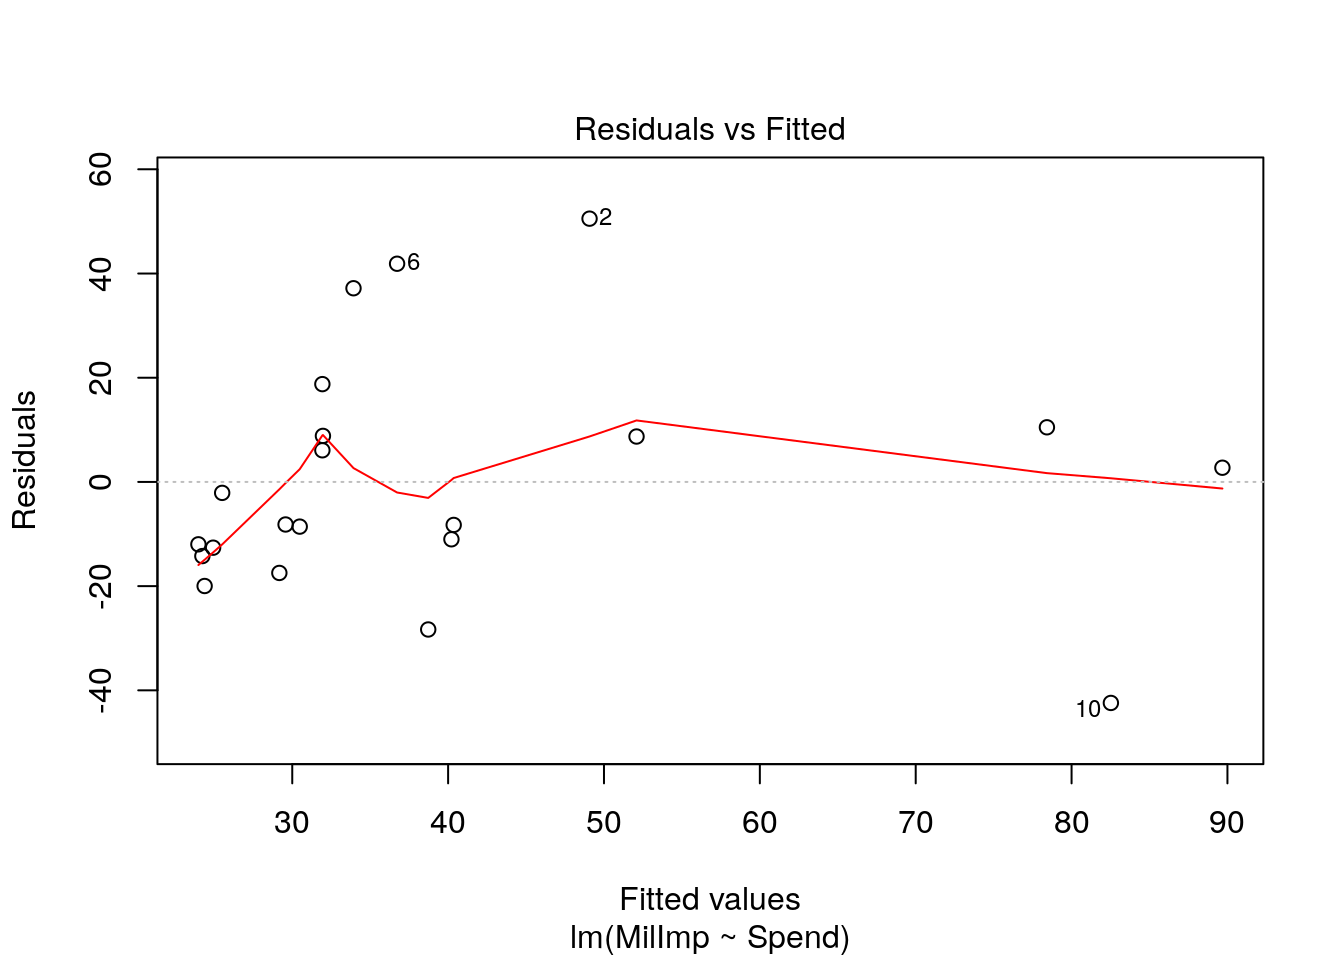
\includegraphics{hw_stat565_files/figure-latex/unnamed-chunk-9-1.pdf}
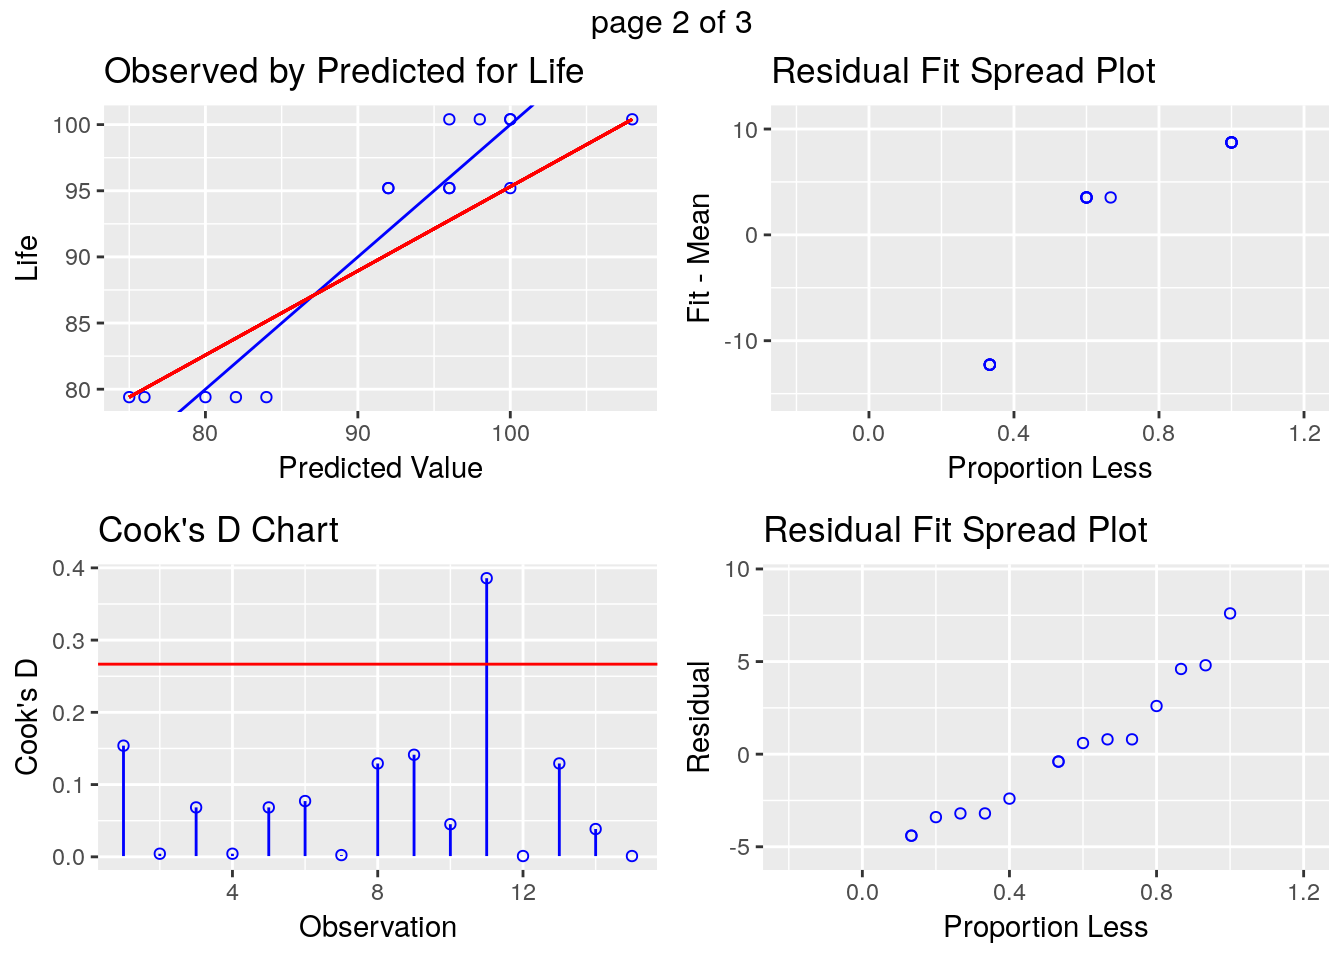
\includegraphics{hw_stat565_files/figure-latex/unnamed-chunk-9-2.pdf}
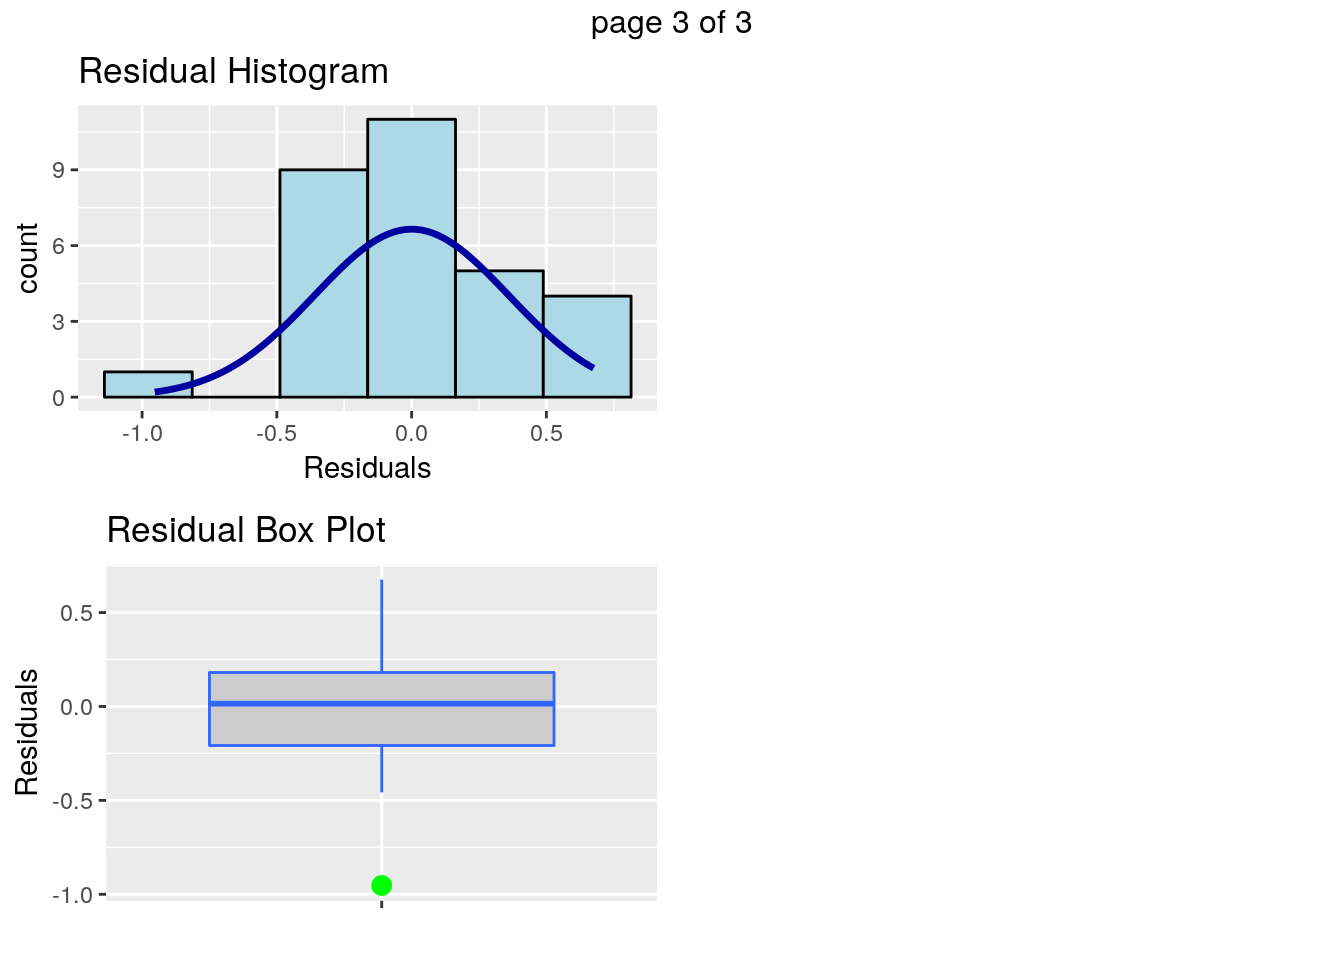
\includegraphics{hw_stat565_files/figure-latex/unnamed-chunk-9-3.pdf}

\begin{Shaded}
\begin{Highlighting}[]
\KeywordTok{bartlett.test}\NormalTok{(Life}\OperatorTok{~}\NormalTok{Brand, }\DataTypeTok{data=}\NormalTok{table_battery)}
\CommentTok{## }
\CommentTok{##  Bartlett test of homogeneity of variances}
\CommentTok{## }
\CommentTok{## data:  Life by Brand}
\CommentTok{## Bartlett's K-squared = 0.34675, df = 2, p-value = 0.8408}
\end{Highlighting}
\end{Shaded}

\begin{center}\rule{0.5\linewidth}{\linethickness}\end{center}

\begin{enumerate}
\def\labelenumi{(\alph{enumi})}
\setcounter{enumi}{2}
\tightlist
\item
  Construct a 95 percent confidence interval estimate on the mean life
  of battery brand 2. Construct a 99 percent confidence interval
  estimate on the mean difference between the lives of battery brands 2
  and 3.
\end{enumerate}

The 95\% confidence interval on the mean life of battery brand 2 is:

\[\bar y_{i.}\pm t_{\frac{\alpha}2,N-a}\sqrt\frac{MS_E}n=79.4\pm t_{\frac{0.05}2,18-3}\sqrt\frac{15.6}5\]

The 99\% confidence interval on the mean difference between the lives of
battery brands 2 and 3 is:

\[\bar y_{i.}-\bar y_{j.}\pm t_{\frac{\alpha}2,N-a}\sqrt\frac{2MS_E}n=79.4-100.4\pm t_{\frac{0.01}2,18-3}\sqrt\frac{2*15.6}5\]

Therefore, \(75.551\le\mu_2\le83.249\),
\(-28.631\le\mu_2-\mu_3\le-13.369\)

\begin{Shaded}
\begin{Highlighting}[]
\NormalTok{(}\KeywordTok{LSD.test}\NormalTok{(model_battery, }\DataTypeTok{trt=}\StringTok{"Brand"}\NormalTok{,}\DataTypeTok{alpha =} \FloatTok{0.05}\NormalTok{))}
\CommentTok{## $statistics}
\CommentTok{##   MSerror Df     Mean       CV  t.value      LSD}
\CommentTok{##      15.6 12 91.66667 4.308746 2.178813 5.442673}
\CommentTok{## }
\CommentTok{## $parameters}
\CommentTok{##         test p.ajusted name.t ntr alpha}
\CommentTok{##   Fisher-LSD      none  Brand   3  0.05}
\CommentTok{## }
\CommentTok{## $means}
\CommentTok{##         Life      std r      LCL       UCL Min Max Q25 Q50 Q75}
\CommentTok{## Brand1  95.2 3.346640 5 91.35145  99.04855  92 100  92  96  96}
\CommentTok{## Brand2  79.4 3.847077 5 75.55145  83.24855  75  84  76  80  82}
\CommentTok{## Brand3 100.4 4.560702 5 96.55145 104.24855  96 108  98 100 100}
\CommentTok{## }
\CommentTok{## $comparison}
\CommentTok{## NULL}
\CommentTok{## }
\CommentTok{## $groups}
\CommentTok{##         Life groups}
\CommentTok{## Brand3 100.4      a}
\CommentTok{## Brand1  95.2      a}
\CommentTok{## Brand2  79.4      b}
\CommentTok{## }
\CommentTok{## attr(,"class")}
\CommentTok{## [1] "group"}
\KeywordTok{pairw.anova}\NormalTok{(table_battery}\OperatorTok{$}\NormalTok{Life,}\KeywordTok{as.factor}\NormalTok{(table_battery}\OperatorTok{$}\NormalTok{Brand), }\DataTypeTok{conf.level =} \FloatTok{0.99}\NormalTok{, }\DataTypeTok{method =} \StringTok{"lsd"}\NormalTok{, }\DataTypeTok{MSE =} \OtherTok{NULL}\NormalTok{, }\DataTypeTok{df.err =} \OtherTok{NULL}\NormalTok{, }\DataTypeTok{control =} \OtherTok{NULL}\NormalTok{)}
\CommentTok{## }
\CommentTok{## 99% LSD confidence intervals }
\CommentTok{## }
\CommentTok{##                       LSD Diff     Lower     Upper  Decision Adj. p-value}
\CommentTok{## muBrand1-muBrand2 7.63024 15.8   8.16976  23.43024 Reject H0        4e-05}
\CommentTok{## muBrand1-muBrand3 7.63024 -5.2 -12.83024   2.43024    FTR H0      0.05945}
\CommentTok{## muBrand2-muBrand3 7.63024  -21 -28.63024 -13.36976 Reject H0            0}
\KeywordTok{bonf.cont}\NormalTok{(table_battery}\OperatorTok{$}\NormalTok{Life,}\KeywordTok{as.factor}\NormalTok{(table_battery}\OperatorTok{$}\NormalTok{Brand), }\DataTypeTok{lvl =} \KeywordTok{c}\NormalTok{(}\StringTok{"Brand2"}\NormalTok{, }\StringTok{"Brand3"}\NormalTok{), }\DataTypeTok{conf.level =} \FloatTok{0.99}\NormalTok{, }\DataTypeTok{MSE =} \OtherTok{NULL}\NormalTok{, }\DataTypeTok{df.err =} \OtherTok{NULL}\NormalTok{, }\DataTypeTok{comps =} \DecValTok{1}\NormalTok{)}
\CommentTok{##                   Diff     Lower     Upper  Decision Adj. P-value}
\CommentTok{## muBrand2-muBrand3  -21 -28.63024 -13.36976 Reject H0 2.254928e-06}
\end{Highlighting}
\end{Shaded}

\begin{center}\rule{0.5\linewidth}{\linethickness}\end{center}

\begin{enumerate}
\def\labelenumi{(\alph{enumi})}
\setcounter{enumi}{3}
\tightlist
\item
  Which brand would you select for use? If the manufacturer will replace
  without charge any battery that fails in less than 85 weeks, what
  percentage would the company expect to replace?
\end{enumerate}

Chose brand 3 for longest life. Mean life of this brand in 100.4 weeks,
and the variance of life is estimated by 15.60 (MSE). Assuming
normality, then the probability of failure before 85 weeks is:

\[Φ\left(\frac{85-100.4}{\sqrt{15.60}}\right)=Φ(-0.390)=0.00005\]

That is, about 5 out of 100,000 batteries will fail before 85 week.

\hypertarget{problem-5-3.2226}{%
\subsubsection{Problem 5 (3.22/26)}\label{problem-5-3.2226}}

The response time in milliseconds was determined for three different
types of circuits that could be used in an automatic valve shutoff
mechanism. The results from a completely randomized experiment are shown
in the following table:

\begin{enumerate}
\def\labelenumi{(\alph{enumi})}
\tightlist
\item
  Test the hypothesis that the three circuit types have the same
  response time. Use 𝛼 = 0.01.
\end{enumerate}

The relevant overall hypotheses are \(H_0: \mu_1=\mu_2=\mu_3, H_1:\) at
lesat two of \(\mu_i\) are different.

The ANOVA result shows that p-value of F-test (\(0.000402\)) is small
enough to reject \(H_0\). We can conclude there is a significant
differce in treatment means or these circuits types have an effect on
the response time on 0.01 significent level.

\begin{Shaded}
\begin{Highlighting}[]
\NormalTok{table_circuit <-}\StringTok{ }\KeywordTok{read_xlsx}\NormalTok{(}\StringTok{"Exercise3_22.xlsx"}\NormalTok{)}
\NormalTok{model_circuit <-}\StringTok{ }\KeywordTok{aov}\NormalTok{(Respone}\OperatorTok{~}\NormalTok{Type, }\DataTypeTok{data=}\NormalTok{table_circuit)}
\KeywordTok{summary}\NormalTok{(model_circuit)}
\CommentTok{##             Df Sum Sq Mean Sq F value   Pr(>F)    }
\CommentTok{## Type         2  543.6   271.8   16.08 0.000402 ***}
\CommentTok{## Residuals   12  202.8    16.9                     }
\CommentTok{## ---}
\CommentTok{## Signif. codes:  0 '***' 0.001 '**' 0.01 '*' 0.05 '.' 0.1 ' ' 1}
\end{Highlighting}
\end{Shaded}

\begin{center}\rule{0.5\linewidth}{\linethickness}\end{center}

\begin{enumerate}
\def\labelenumi{(\alph{enumi})}
\setcounter{enumi}{1}
\tightlist
\item
  Use Tukey's test to compare pairs of treatment means. Use 𝛼 = 0.01.
\end{enumerate}

Let \(H_{(1-2)0}:\mu_1-\mu_2=0,H_{(1-2)1}:\mu_1-\mu_2\neq0\);
\(H_{(1-3)0}:\mu_1-\mu_3=0,H_{(1-3)1}:\mu_1-\mu_3\neq0\);\(H_{(2-3)0}:\mu_2-\mu_3=0,H_{(2-3)1}:\mu_2-\mu_3\neq0\);

The P-values of F-test are
\(P_{(1-2)}=0.0.002366, P_{(1-3)}=0.636704, P_{(2-3)}=0.000504\). We can
reject \(H_{(1-2)0}\) and \(H_{(2-3)0}\), but fail to reject
\(H_{(1-3)0}\). We can conclude treatment means of type 1 and type 2,
treatment means of type 2 and type 3 has a significant differce on 0.01
significent level. There is not significant differce between type 1 and
type 3 on 0.01 significent level.

\begin{Shaded}
\begin{Highlighting}[]
\KeywordTok{TukeyHSD}\NormalTok{(}\KeywordTok{aov}\NormalTok{(model_circuit), }\DataTypeTok{ordered =} \OtherTok{TRUE}\NormalTok{,}\DataTypeTok{conf.level=}\FloatTok{0.99}\NormalTok{)}
\CommentTok{##   Tukey multiple comparisons of means}
\CommentTok{##     99% family-wise confidence level}
\CommentTok{##     factor levels have been ordered}
\CommentTok{## }
\CommentTok{## Fit: aov(formula = model_circuit)}
\CommentTok{## }
\CommentTok{## $Type}
\CommentTok{##             diff       lwr      upr     p adj}
\CommentTok{## Type1-Type3  2.4 -6.876837 11.67684 0.6367043}
\CommentTok{## Type2-Type3 13.8  4.523163 23.07684 0.0005042}
\CommentTok{## Type2-Type1 11.4  2.123163 20.67684 0.0023656}
\KeywordTok{pairw.anova}\NormalTok{(table_circuit}\OperatorTok{$}\NormalTok{Respone,}\KeywordTok{as.factor}\NormalTok{(table_circuit}\OperatorTok{$}\NormalTok{Type), }\DataTypeTok{conf.level =} \FloatTok{0.99}\NormalTok{, }\DataTypeTok{method =} \StringTok{"tukey"}\NormalTok{, }\DataTypeTok{MSE =} \OtherTok{NULL}\NormalTok{, }\DataTypeTok{df.err =} \OtherTok{NULL}\NormalTok{, }\DataTypeTok{control =} \OtherTok{NULL}\NormalTok{)}
\CommentTok{## }
\CommentTok{## 99% Tukey-Kramer confidence intervals }
\CommentTok{## }
\CommentTok{##                  Diff     Lower    Upper  Decision Adj. p-value}
\CommentTok{## muType1-muType2 -11.4 -20.67684 -2.12316 Reject H0     0.002366}
\CommentTok{## muType1-muType3   2.4  -6.87684 11.67684    FTR H0     0.636704}
\CommentTok{## muType2-muType3  13.8   4.52316 23.07684 Reject H0     0.000504}
\end{Highlighting}
\end{Shaded}

\begin{center}\rule{0.5\linewidth}{\linethickness}\end{center}

\begin{enumerate}
\def\labelenumi{(\alph{enumi})}
\setcounter{enumi}{3}
\tightlist
\item
  Construct a set of orthogonal contrasts, assuming that at the outset
  of the experiment you suspected the response time of circuit type 2 to
  be different from the other two.
\end{enumerate}

Construct a set of contrasts
\(\sum_{i=1}^3c_i=1-2+1=0,\sum_{i=1}^3d_i=1+0-1=0\)

\[\begin{cases}\mu_1-2\mu_2+\mu_3=0\\\mu_1-\mu_3=0\end{cases}\]

For \(\sum_{i=1}^3c_id_i=1*1+(-2)*0+1*(-1)=0\), they are orthogonal
contrasts.

\[C=\sum_{i=1}^ac_i\bar y_{i.}=\bar y_{1.}-2\bar y_{2.}+\bar y_{3.}=10.8-2(22.2)+8.4=-25.2\]

\[H_{C0}:\mu_1-2\mu_2+\mu_3=0\quad H_{C1}:\mu_1-2\mu_2+\mu_3\neq0\]

\[F_{1,12}=\frac{SS_C}{MS_E}=\frac{C^2}{\frac{MS_E}n\sum_{i=1}^ac_i^2}=\frac{(-25.2)^2}{\frac{16.9}56}=31.31\]

For the first contrast, the P-value of F-test (\(0.0001169669\)) is
small enough to reject \(H_{C0}\), We can conclude treatment means of
type 2 has a significant differenence with treatment means of type 1 and
type 3 on 0.01 significent level.

\[D=\sum_{i=1}^ac_i\bar y_{i.}=\bar y_{1.}-\bar y_{3.}=10.8-8.4=2.4\]

\[H_{D0}:\mu_1-\mu_3=0\quad H_{D1}:\mu_1-\mu_3\neq0\]

\[F_{1,12}=\frac{SS_C}{MS_E}=\frac{C^2}{\frac{MS_E}n\sum_{i=1}^ac_i^2}=\frac{2.4^2}{\frac{16.9}52}=0.852071\]

For the second contrast, the P-value of F-test (\(0.374155\)) is large
and fail to reject \(H_{D0}\), We can conclude there is not a
significant differce between treatment means of type 1 and type 3 on
0.01 significent level.

\begin{Shaded}
\begin{Highlighting}[]
\KeywordTok{HSD.test}\NormalTok{(model_circuit,}\StringTok{"Type"}\NormalTok{, }\DataTypeTok{group=}\OtherTok{TRUE}\NormalTok{,}\DataTypeTok{console=}\OtherTok{TRUE}\NormalTok{)}
\CommentTok{## }
\CommentTok{## Study: model_circuit ~ "Type"}
\CommentTok{## }
\CommentTok{## HSD Test for Respone }
\CommentTok{## }
\CommentTok{## Mean Square Error:  16.9 }
\CommentTok{## }
\CommentTok{## Type,  means}
\CommentTok{## }
\CommentTok{##       Respone      std r Min Max}
\CommentTok{## Type1    10.8 2.774887 5   8  15}
\CommentTok{## Type2    22.2 4.868265 5  17  30}
\CommentTok{## Type3     8.4 4.393177 5   5  16}
\CommentTok{## }
\CommentTok{## Alpha: 0.05 ; DF Error: 12 }
\CommentTok{## Critical Value of Studentized Range: 3.772929 }
\CommentTok{## }
\CommentTok{## Minimun Significant Difference: 6.936445 }
\CommentTok{## }
\CommentTok{## Treatments with the same letter are not significantly different.}
\CommentTok{## }
\CommentTok{##       Respone groups}
\CommentTok{## Type2    22.2      a}
\CommentTok{## Type1    10.8      b}
\CommentTok{## Type3     8.4      b}

\NormalTok{(}\FloatTok{25.2}\OperatorTok{^}\DecValTok{2}\OperatorTok{*}\DecValTok{5}\NormalTok{)}\OperatorTok{/}\NormalTok{(}\FloatTok{16.9}\OperatorTok{*}\DecValTok{6}\NormalTok{)}
\CommentTok{## [1] 31.31361}
\NormalTok{(}\FloatTok{2.4}\OperatorTok{^}\DecValTok{2}\OperatorTok{*}\DecValTok{5}\NormalTok{)}\OperatorTok{/}\NormalTok{(}\FloatTok{16.9}\OperatorTok{*}\DecValTok{2}\NormalTok{)}
\CommentTok{## [1] 0.852071}

\KeywordTok{qf}\NormalTok{(}\FloatTok{0.95}\NormalTok{, }\DecValTok{1}\NormalTok{, }\DecValTok{12}\NormalTok{, }\DataTypeTok{lower.tail =} \OtherTok{TRUE}\NormalTok{, }\DataTypeTok{log.p =} \OtherTok{FALSE}\NormalTok{)}
\CommentTok{## [1] 4.747225}
\DecValTok{1}\OperatorTok{-}\KeywordTok{pf}\NormalTok{(}\FloatTok{31.31}\NormalTok{, }\DecValTok{1}\NormalTok{, }\DecValTok{12}\NormalTok{, }\DataTypeTok{lower.tail =} \OtherTok{TRUE}\NormalTok{, }\DataTypeTok{log.p =} \OtherTok{FALSE}\NormalTok{)}
\CommentTok{## [1] 0.0001169669}
\DecValTok{1}\OperatorTok{-}\KeywordTok{pf}\NormalTok{(}\FloatTok{0.852071}\NormalTok{, }\DecValTok{1}\NormalTok{, }\DecValTok{12}\NormalTok{, }\DataTypeTok{lower.tail =} \OtherTok{TRUE}\NormalTok{, }\DataTypeTok{log.p =} \OtherTok{FALSE}\NormalTok{)}
\CommentTok{## [1] 0.374155}
\end{Highlighting}
\end{Shaded}

\begin{center}\rule{0.5\linewidth}{\linethickness}\end{center}

\begin{enumerate}
\def\labelenumi{(\alph{enumi})}
\setcounter{enumi}{4}
\tightlist
\item
  If you were the design engineer and you wished to minimize the
  response time, which circuit type would you select?
\end{enumerate}

Type 1 and type 3 have lower response time (\(\mu_1=10.8,\mu_3=8.4\)).
We had proved the mean of response time for type 1 and type 3 have not
significant different on response time on 0.01 significant level. The
engineer could choose either one.

\begin{center}\rule{0.5\linewidth}{\linethickness}\end{center}

\begin{enumerate}
\def\labelenumi{(\alph{enumi})}
\setcounter{enumi}{5}
\tightlist
\item
  Analyze the residuals from this experiment. Are the basic analysis of
  variance assumptions satisfied?
\end{enumerate}

\begin{itemize}
\tightlist
\item
  The histogram doesn't show a quite normality of of residuals.
\item
  The QQ plot of residuals shows some violaion of normality of
  residuals. The respnse variable may need to be transformed.
\item
  The residuals versus fitted values and studentized residuals show no
  violation of zero mean and constant variance assumptions.
\item
  There are some outlier and leverage data points.
\item
  Compared with the Bartlett's test , the Levene test is less sensitive
  to departures from normality. The result shows variances across
  samples may be equal.
\end{itemize}

Therefore, we should check the outlier points and try to do some
transfoation.

\begin{Shaded}
\begin{Highlighting}[]
\KeywordTok{ols_plot_diagnostics}\NormalTok{(}\KeywordTok{lm}\NormalTok{(Respone}\OperatorTok{~}\NormalTok{Type, }\DataTypeTok{data=}\NormalTok{table_circuit))}
\end{Highlighting}
\end{Shaded}

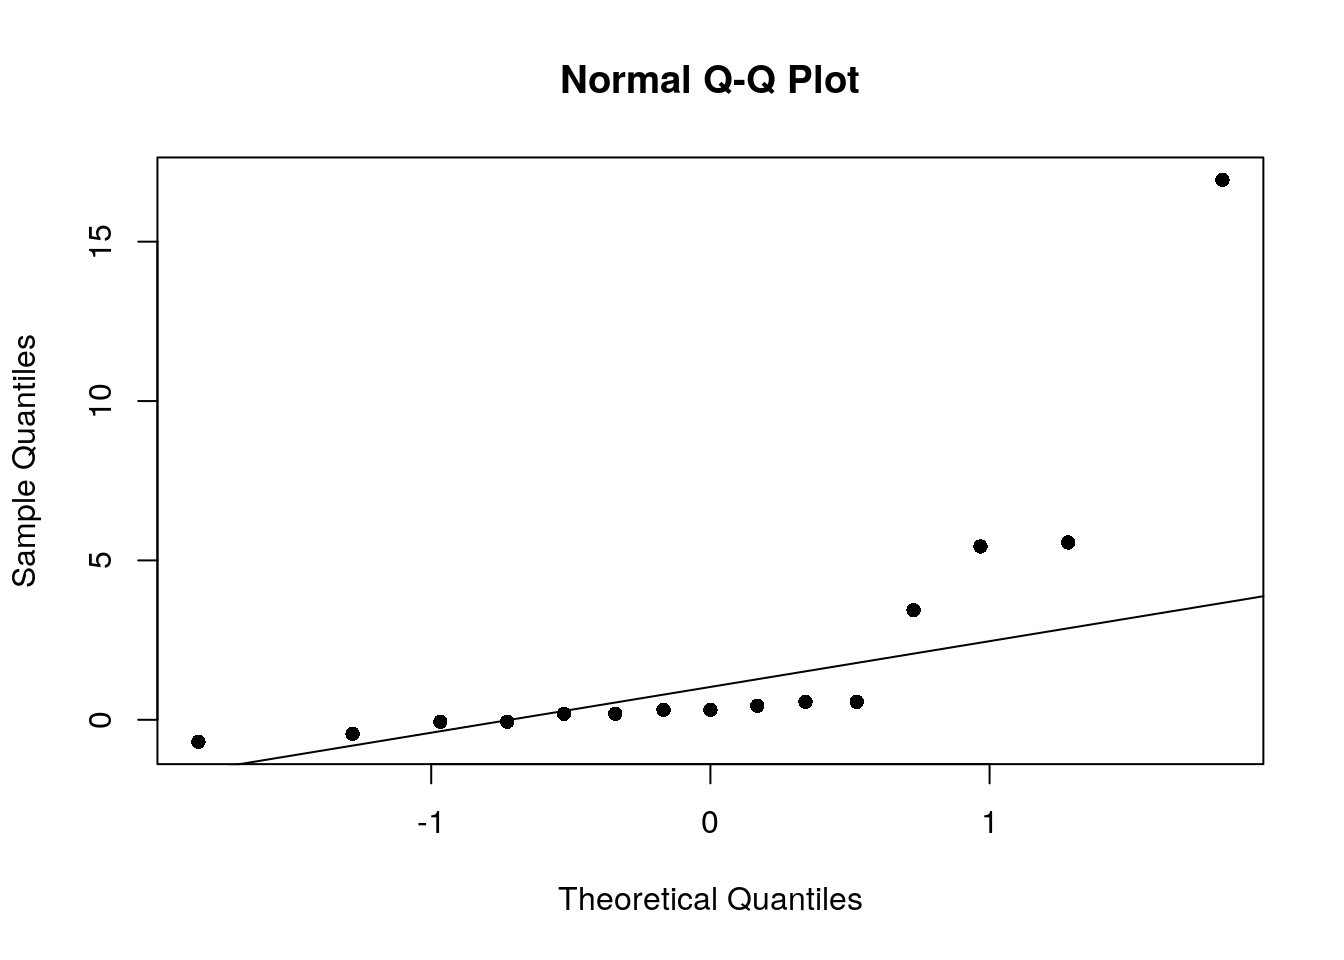
\includegraphics{hw_stat565_files/figure-latex/unnamed-chunk-14-1.pdf}
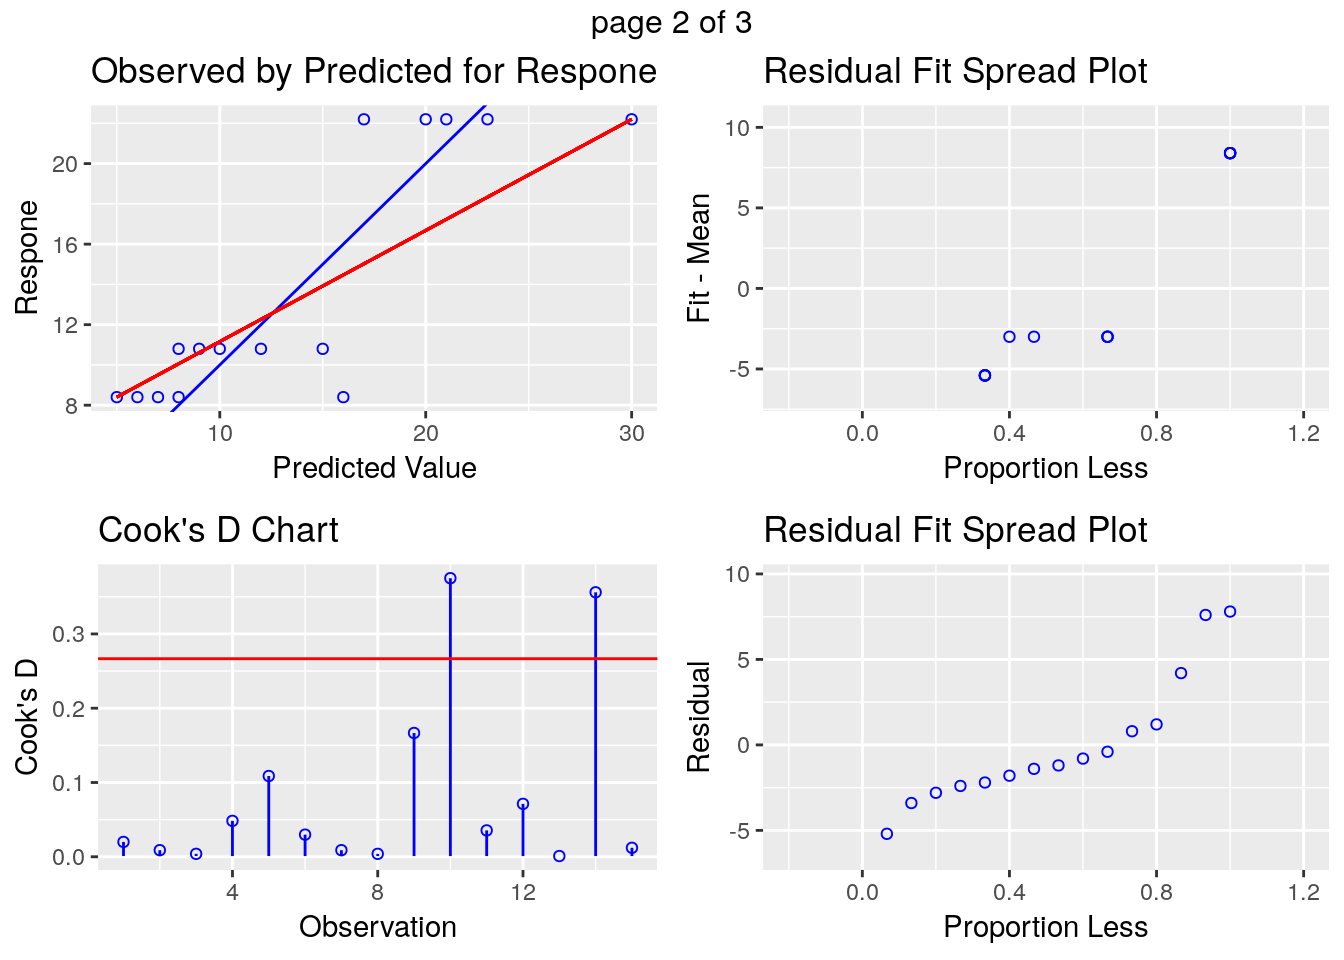
\includegraphics{hw_stat565_files/figure-latex/unnamed-chunk-14-2.pdf}
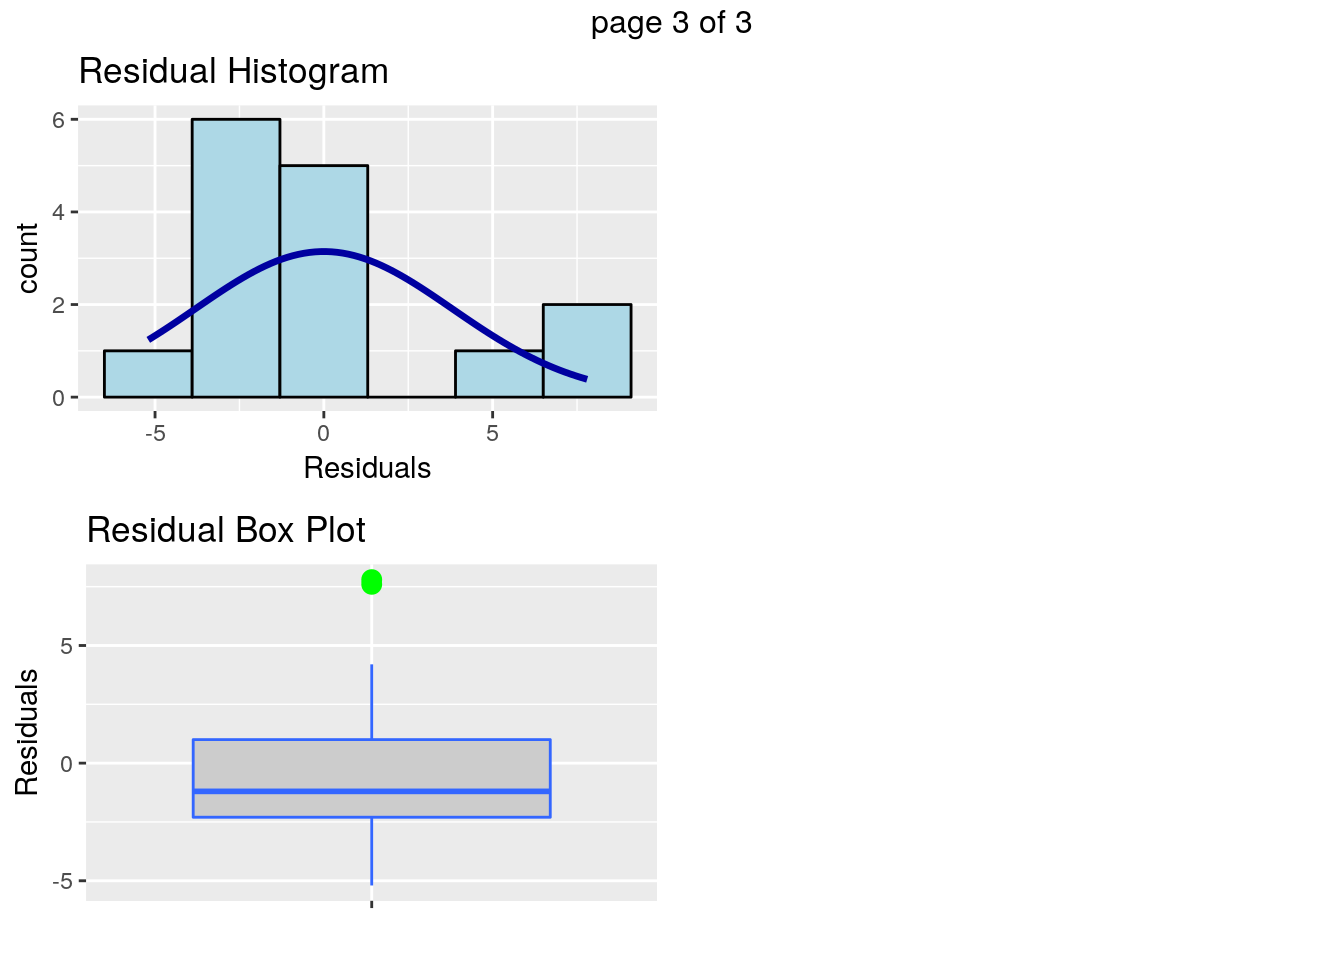
\includegraphics{hw_stat565_files/figure-latex/unnamed-chunk-14-3.pdf}

\begin{Shaded}
\begin{Highlighting}[]
\KeywordTok{bartlett.test}\NormalTok{(Respone}\OperatorTok{~}\NormalTok{Type, }\DataTypeTok{data=}\NormalTok{table_circuit)}
\CommentTok{## }
\CommentTok{##  Bartlett test of homogeneity of variances}
\CommentTok{## }
\CommentTok{## data:  Respone by Type}
\CommentTok{## Bartlett's K-squared = 1.1345, df = 2, p-value = 0.5671}
\KeywordTok{leveneTest}\NormalTok{(model_circuit)}
\CommentTok{## Warning in leveneTest.default(y = y, group = group, ...): group coerced to}
\CommentTok{## factor.}
\CommentTok{## Levene's Test for Homogeneity of Variance (center = median)}
\CommentTok{##       Df F value Pr(>F)}
\CommentTok{## group  2  0.1831  0.835}
\CommentTok{##       12}
\end{Highlighting}
\end{Shaded}

\hypertarget{problem-6-3.419-and-3.4957}{%
\subsubsection{Problem 6: (3.41/9 and
3.49/57)}\label{problem-6-3.419-and-3.4957}}

(3.41/9) Refer to Problem 5. If we wish to detect a maximum difference
in mean response times of 10 milliseconds with a probability of at least
0.90, what sample size should be used? How would you obtain a
preliminary estimate of \(σ^2\)?

For \(a=3, D=10\), the preliminary estimate \(\hat\sigma^2=MS_E=16.9\).

\[Φ^2=\frac{nD^2}{2aσ^2}=\frac{n(10)^2}{2(3)(16.9)}=0.986n\]

Let \(α=0.05\), accept probability \(P=0.1,\nu_1=a−1=2\)

The results show that when \(n=5\), the power is 0.86476, when \(n=6\),
the power is 0.9345867. Thus, the sample size should be
\(n\ge6, N\ge18\).

\begin{Shaded}
\begin{Highlighting}[]
\KeywordTok{library}\NormalTok{(pwr2)}
\KeywordTok{pwr.1way}\NormalTok{(}\DataTypeTok{k=}\DecValTok{3}\NormalTok{, }\DataTypeTok{n=}\DecValTok{5}\NormalTok{, }\DataTypeTok{alpha=}\FloatTok{0.05}\NormalTok{, }\DataTypeTok{f=}\OtherTok{NULL}\NormalTok{, }\DataTypeTok{delta=}\DecValTok{10}\NormalTok{, }\DataTypeTok{sigma=}\KeywordTok{sqrt}\NormalTok{(}\FloatTok{16.9}\NormalTok{))}
\CommentTok{## }
\CommentTok{##      Balanced one-way analysis of variance power calculation }
\CommentTok{## }
\CommentTok{##               k = 3}
\CommentTok{##               n = 5}
\CommentTok{##           delta = 10}
\CommentTok{##           sigma = 4.110961}
\CommentTok{##     effect.size = 0.9930727}
\CommentTok{##       sig.level = 0.05}
\CommentTok{##           power = 0.86476}
\CommentTok{## }
\CommentTok{## }\AlertTok{NOTE}\CommentTok{: n is number in each group, total sample = 15 power = 0.864759967690655}
\KeywordTok{pwr.1way}\NormalTok{(}\DataTypeTok{k=}\DecValTok{3}\NormalTok{, }\DataTypeTok{n=}\DecValTok{6}\NormalTok{, }\DataTypeTok{alpha=}\FloatTok{0.05}\NormalTok{, }\DataTypeTok{f=}\OtherTok{NULL}\NormalTok{, }\DataTypeTok{delta=}\DecValTok{10}\NormalTok{, }\DataTypeTok{sigma=}\KeywordTok{sqrt}\NormalTok{(}\FloatTok{16.9}\NormalTok{))}
\CommentTok{## }
\CommentTok{##      Balanced one-way analysis of variance power calculation }
\CommentTok{## }
\CommentTok{##               k = 3}
\CommentTok{##               n = 6}
\CommentTok{##           delta = 10}
\CommentTok{##           sigma = 4.110961}
\CommentTok{##     effect.size = 0.9930727}
\CommentTok{##       sig.level = 0.05}
\CommentTok{##           power = 0.9345867}
\CommentTok{## }
\CommentTok{## }\AlertTok{NOTE}\CommentTok{: n is number in each group, total sample = 18 power = 0.934586703973552}
\end{Highlighting}
\end{Shaded}

\begin{center}\rule{0.5\linewidth}{\linethickness}\end{center}

(3.49/57) Consider the data shown in Problem 5.

\begin{enumerate}
\def\labelenumi{(\alph{enumi})}
\tightlist
\item
  Write out the least squares normal equations for this problem and
  solve them for \(\hat\mu\) and \(\hat\tau_i\), using the usual
  constraint (\(\sum^3_{i=1} \hat\tau_i=0\)). Estimate \(\tau_1-\tau_2\)
\end{enumerate}

For \(\sum^3_{i=1} \hat\tau_i=0\),

\[\begin{cases}\hat\tau_1+\hat\tau_2+\hat\tau_3=0\\\hat\mu+\hat\tau_1=\bar y_{1.}=10.8\\\hat\mu+\hat\tau_2=\bar y_{2.}=22.2\\\hat\mu+\hat\tau_3=\bar y_{3.}=8.4\end{cases}\implies
\begin{cases}\hat\mu=13.80\\\hat\tau_1=-3.00\\\hat\tau_2=8.40\\\hat\tau_3=-5.40\end{cases}\implies
\hat\tau_1-\hat\tau_2=-11.40\]

\begin{center}\rule{0.5\linewidth}{\linethickness}\end{center}

\begin{enumerate}
\def\labelenumi{(\alph{enumi})}
\setcounter{enumi}{1}
\tightlist
\item
  Solve the equations in (a) using the constraint \(\hat\tau_3=0\). Are
  the estimator \(\hat\tau_i\) and \(\hat\mu\) the same as you found in
  (a)? Why? Now estimate \(\tau_1-\tau_2\) and compare your answer with
  that for (a). What statement can you make about estimating contrasts
  in the \(\tau_i\)
\end{enumerate}

\[\begin{cases}\hat\tau_3=0\\\hat\mu+\hat\tau_1=\bar y_{1.}=10.8\\\hat\mu+\hat\tau_2=\bar y_{2.}=22.2\\\hat\mu+\hat\tau_3=\bar y_{3.}=8.4\end{cases}\implies
\begin{cases}\hat\mu=8.40\\\hat\tau_1=2.40\\\hat\tau_2=13.8\\\hat\tau_3=0\end{cases}\implies
\hat\tau_1-\hat\tau_2=-11.40\]

The result shows the value of \(\hatτ_1-\hatτ_2\) is irrelevant with the
value of \(\hatτ_3\). The contrasts are estimable.

\begin{center}\rule{0.5\linewidth}{\linethickness}\end{center}

\begin{enumerate}
\def\labelenumi{(\alph{enumi})}
\setcounter{enumi}{2}
\tightlist
\item
  Estimate \(\mu+\tau_1\), \(2\tau_1-\tau_2-\tau_3\), and
  \(\mu+\tau_1+\tau_2\) using the two solutions to the normal equations.
  Compare the results obtained in each case.
\end{enumerate}

\begin{longtable}[]{@{}lll@{}}
\toprule
Contrast & Estimated from Part (a) & Estimated from Part
(b)\tabularnewline
\midrule
\endhead
\(\mu+\tau_1\) & 10.80 & 10.80\tabularnewline
\(2\tau_1-\tau_2-\tau_3\) & -9.00 & -9.00\tabularnewline
\(\mu+\tau_1+\tau_2\) & 19.20 & 24.60\tabularnewline
\bottomrule
\end{longtable}

The result shows that \(\tau_1\) is independent with \(\tau_3\),
\(\tau_1\) is independent with \(\tau_2\) and \(\tau_3\), while
\(\tau_1\) and \(\tau_2\) is dependent with \(\tau_3\).

\hypertarget{hw2}{%
\subsection{HW2}\label{hw2}}

\hypertarget{problem-1-4.9-29}{%
\subsubsection{Problem 1 (4.9-29)}\label{problem-1-4.9-29}}

Three different washing solutions are being compared to study their
effectiveness in retarding bacteria growth in 5-gallon milk containers.
The analysis is done in a laboratory, and only three trials can be run
on any day. Because days could represent a potential source of
variability, the experimenter decides to use a randomized block design.
Observations are taken for four days, and the data are shown here.
Analyze the data from this experiment (use \(\alpha = 0.05\)) and draw
conclusions.

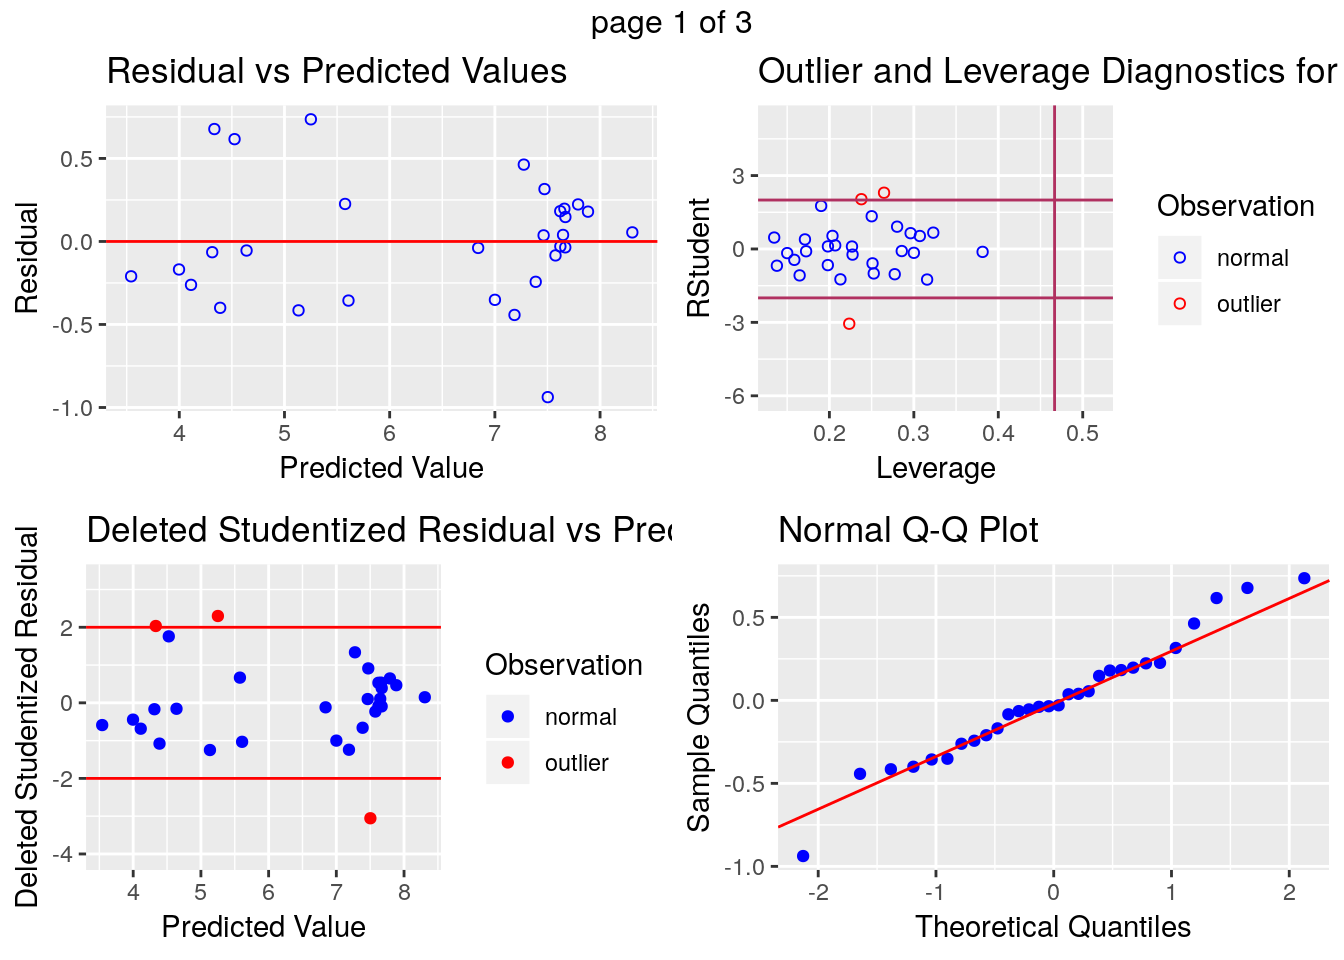
\includegraphics[width=0.45\linewidth]{hw_stat565_files/figure-latex/unnamed-chunk-18-1}

\begin{verbatim}
## Observations: 12
## Variables: 3
## $ Days     <fct> 1, 1, 1, 2, 2, 2, 3, 3, 3, 4, 4, 4
## $ Solution <fct> 1, 2, 3, 1, 2, 3, 1, 2, 3, 1, 2, 3
## $ Response <dbl> 13, 16, 5, 22, 24, 4, 18, 17, 1, 39, 44, 22
\end{verbatim}

\begin{itemize}
\tightlist
\item
  The overall results
\end{itemize}

The ANOVA for RCBD shows that both treatments of solutions and blocks of
days have significant effects on the average values of bacteria growth
at 0.05 significant level. The P-value for treatment is 0.000323 while
it for days is 0.000192.

The results of estimating regression coefficients show the P-value of
Solution1 and Days1(0.000291), Solution3(0.000359), Days4(0.0000627) are
small enough, while the P-value of Solution2(0.320563), Days2(0.067976),
and Days3(0.790493) are larger than 0.05. The coefficients of Solution1,
Days1, Solution3, Days4 are significant at 0.05 significant level. The
rest are not.

\begin{itemize}
\tightlist
\item
  Comparing the treatment effects
\end{itemize}

The plot of LSD test shows the average response value for Solution3 has
a different interval with that for other solutions. The Tukey test also
shows the average response values for Solution3 are significant
different with Solution1(P-value=0.0008758) and
Solution2(P-value=0.0004067) at 0.05 significant level, while there is
not significant difference between the average response values for
Solution1 and Solution2(P-value=0.5577862) at 0.05 significant level.

However, the results by another code ``pairw.anova'' didn't reveal
significant difference among the three solutions in both LSD and Tukey
methods. I'm still looking for the reason.

\begin{itemize}
\tightlist
\item
  Comparing the block effects
\end{itemize}

The plot of LSD test shows the average response value for Days4 has a
different interval with that for other Days. The Tukey test also shows
the average response values for Days4 are significant different with
Days1(P-value=0.0002622,), Days2(P-value=0.0010843) and
Days3(P-value=0.0003081) at 0.05 significant level, while there is not
significant difference between the average response values for Days1,
Days2, and Days3(P-value: 1-2=0.2193500, 1-3=0.9917442, 2-3=0.3037891)
at 0.05 significant level.

Using the code ``pairw.anova'', The LSD method gave the same result with
``TukeyHSD'' but the Tukey method didn't find significant difference
among the four days at 0.05 significant level. I'm still looking for the
reason.

\begin{itemize}
\tightlist
\item
  Model adequacy Checking
\end{itemize}

There is a little bit of violation of normality in histogram plot. The
QQ plot has a little bit of heavier left tail. The residuals versus
fitted values shows a slight curved plot. Studentized residuals show
some violation of zero mean and constant variance assumptions. This
could mean that other regressor variables are needed in the model.
Transformations on the regressor or the response variable may also be
helpful. There is not serious outlier and leverage data points. The
residuals versus observation number shows the residuals are independent
with each other.

\begin{itemize}
\tightlist
\item
  The initial conculsion
\end{itemize}

Based on the experimental data, we found Solution3 has a stronger
effectiveness in retarding bacteria growth in 5-gallon milk containers.
Meanwhile, the data in Days4 are significant different with others. Next
step, We suggest to investigate the factors affecting the data, refine
the design, and repeat the experiment.

\begin{Shaded}
\begin{Highlighting}[]
\NormalTok{model_wash <-}\StringTok{ }\KeywordTok{aov}\NormalTok{(Response}\OperatorTok{~}\NormalTok{Solution}\OperatorTok{+}\NormalTok{Days, }\DataTypeTok{data=}\NormalTok{table_wash)}
\KeywordTok{summary}\NormalTok{(model_wash)}
\end{Highlighting}
\end{Shaded}

\begin{verbatim}
##             Df Sum Sq Mean Sq F value   Pr(>F)    
## Solution     2  703.5   351.8   40.72 0.000323 ***
## Days         3 1106.9   369.0   42.71 0.000192 ***
## Residuals    6   51.8     8.6                     
## ---
## Signif. codes:  0 '***' 0.001 '**' 0.01 '*' 0.05 '.' 0.1 ' ' 1
\end{verbatim}

\begin{Shaded}
\begin{Highlighting}[]
\KeywordTok{summary.lm}\NormalTok{(model_wash)}
\end{Highlighting}
\end{Shaded}

\begin{verbatim}
## 
## Call:
## aov(formula = Response ~ Solution + Days, data = table_wash)
## 
## Residuals:
##    Min     1Q Median     3Q    Max 
## -2.583 -1.854 -0.250  1.250  4.417 
## 
## Coefficients:
##             Estimate Std. Error t value Pr(>|t|)    
## (Intercept)  15.5833     2.0783   7.498 0.000291 ***
## Solution2     2.2500     2.0783   1.083 0.320563    
## Solution3   -15.0000     2.0783  -7.217 0.000359 ***
## Days2         5.3333     2.3998   2.222 0.067976 .  
## Days3         0.6667     2.3998   0.278 0.790493    
## Days4        23.6667     2.3998   9.862 6.27e-05 ***
## ---
## Signif. codes:  0 '***' 0.001 '**' 0.01 '*' 0.05 '.' 0.1 ' ' 1
## 
## Residual standard error: 2.939 on 6 degrees of freedom
## Multiple R-squared:  0.9722, Adjusted R-squared:  0.949 
## F-statistic: 41.91 on 5 and 6 DF,  p-value: 0.0001371
\end{verbatim}

\begin{Shaded}
\begin{Highlighting}[]
\CommentTok{# Plot for solutions and days}
\KeywordTok{plot}\NormalTok{(}\KeywordTok{LSD.test}\NormalTok{(model_wash, }\DataTypeTok{trt=}\StringTok{"Solution"}\NormalTok{,}\DataTypeTok{alpha =} \FloatTok{0.05}\NormalTok{,}\DataTypeTok{p.adj=}\StringTok{"bonferroni"}\NormalTok{),}\DataTypeTok{main=}\StringTok{"Ranges of response grouped by solutions"}\NormalTok{)}
\KeywordTok{plot}\NormalTok{(}\KeywordTok{LSD.test}\NormalTok{(}\KeywordTok{aov}\NormalTok{(Response}\OperatorTok{~}\NormalTok{Days}\OperatorTok{+}\NormalTok{Solution, }\DataTypeTok{data=}\NormalTok{table_wash), }\DataTypeTok{trt=}\StringTok{"Days"}\NormalTok{,}\DataTypeTok{alpha =} \FloatTok{0.05}\NormalTok{,}\DataTypeTok{p.adj=}\StringTok{"bonferroni"}\NormalTok{),}\DataTypeTok{main=}\StringTok{"Ranges of response grouped by days"}\NormalTok{)}
\end{Highlighting}
\end{Shaded}

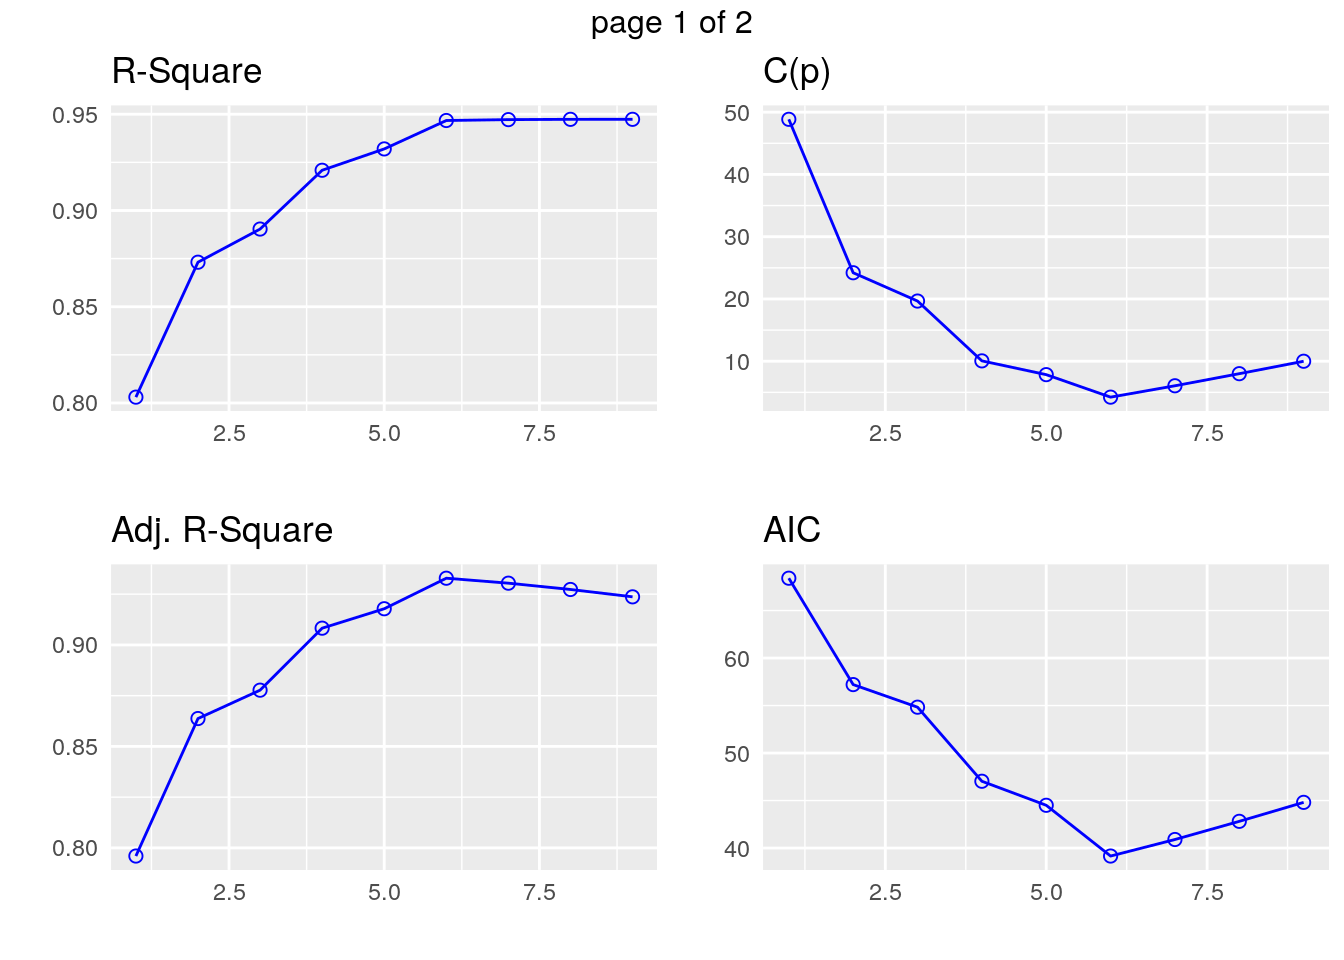
\includegraphics[width=0.3\linewidth]{hw_stat565_files/figure-latex/unnamed-chunk-20-1}
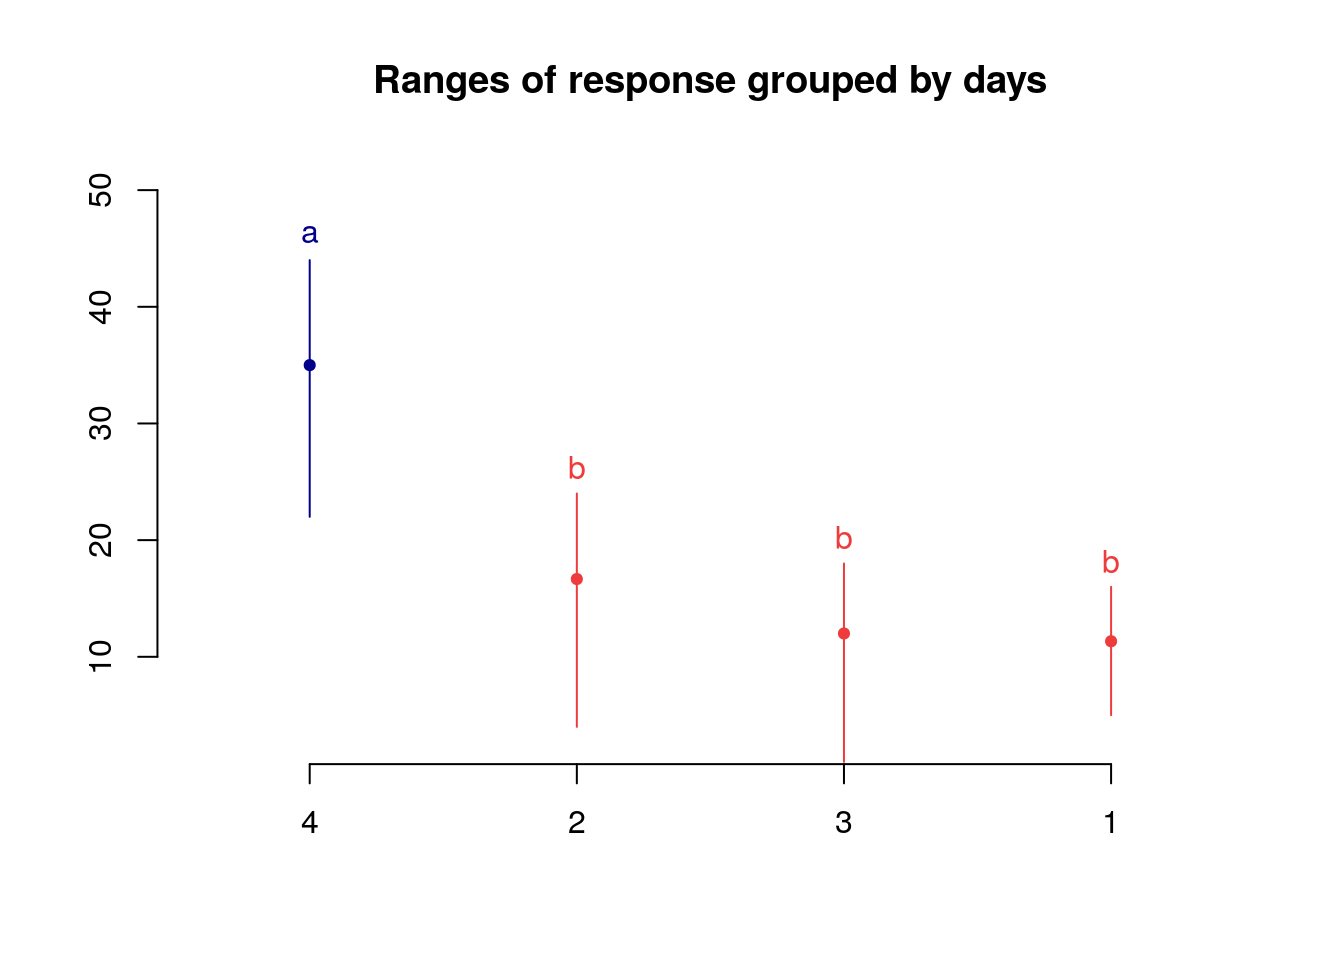
\includegraphics[width=0.3\linewidth]{hw_stat565_files/figure-latex/unnamed-chunk-20-2}

\begin{Shaded}
\begin{Highlighting}[]
\CommentTok{# Comparison of solutions}
\KeywordTok{TukeyHSD}\NormalTok{(model_wash,}\DataTypeTok{conf.level =} \FloatTok{0.95}\NormalTok{)}
\end{Highlighting}
\end{Shaded}

\begin{verbatim}
##   Tukey multiple comparisons of means
##     95% family-wise confidence level
## 
## Fit: aov(formula = Response ~ Solution + Days, data = table_wash)
## 
## $Solution
##       diff        lwr        upr     p adj
## 2-1   2.25  -4.126879   8.626879 0.5577862
## 3-1 -15.00 -21.376879  -8.623121 0.0008758
## 3-2 -17.25 -23.626879 -10.873121 0.0004067
## 
## $Days
##           diff        lwr       upr     p adj
## 2-1  5.3333333  -2.974240 13.640906 0.2193500
## 3-1  0.6666667  -7.640906  8.974240 0.9917442
## 4-1 23.6666667  15.359094 31.974240 0.0002622
## 3-2 -4.6666667 -12.974240  3.640906 0.3037891
## 4-2 18.3333333  10.025760 26.640906 0.0010843
## 4-3 23.0000000  14.692427 31.307573 0.0003081
\end{verbatim}

\begin{Shaded}
\begin{Highlighting}[]
\KeywordTok{pairw.anova}\NormalTok{(table_wash}\OperatorTok{$}\NormalTok{Response,table_wash}\OperatorTok{$}\NormalTok{Solution, }\DataTypeTok{conf.level =} \FloatTok{0.95}\NormalTok{, }\DataTypeTok{method =} \StringTok{"lsd"}\NormalTok{, }\DataTypeTok{MSE =} \OtherTok{NULL}\NormalTok{, }\DataTypeTok{df.err =} \OtherTok{NULL}\NormalTok{, }\DataTypeTok{control =} \OtherTok{NULL}\NormalTok{)}
\end{Highlighting}
\end{Shaded}

\begin{verbatim}
## 
## 95% LSD confidence intervals 
## 
##             LSD  Diff    Lower   Upper Decision Adj. p-value
## mu1-mu2 18.1502 -2.25 -20.4002 15.9002   FTR H0      0.78549
## mu1-mu3 18.1502    15  -3.1502 33.1502   FTR H0      0.09437
## mu2-mu3 18.1502 17.25  -0.9002 35.4002   FTR H0      0.06004
\end{verbatim}

\begin{Shaded}
\begin{Highlighting}[]
\KeywordTok{pairw.anova}\NormalTok{(table_wash}\OperatorTok{$}\NormalTok{Response,table_wash}\OperatorTok{$}\NormalTok{Solution, }\DataTypeTok{conf.level =} \FloatTok{0.95}\NormalTok{, }\DataTypeTok{method =} \StringTok{"tukey"}\NormalTok{, }\DataTypeTok{MSE =} \OtherTok{NULL}\NormalTok{, }\DataTypeTok{df.err =} \OtherTok{NULL}\NormalTok{, }\DataTypeTok{control =} \OtherTok{NULL}\NormalTok{)}
\end{Highlighting}
\end{Shaded}

\begin{verbatim}
## 
## 95% Tukey-Kramer confidence intervals 
## 
##          Diff     Lower    Upper Decision Adj. p-value
## mu1-mu2 -2.25 -24.65139 20.15139   FTR H0     0.957777
## mu1-mu3    15  -7.40139 37.40139   FTR H0     0.202758
## mu2-mu3 17.25  -5.15139 39.65139   FTR H0     0.134327
\end{verbatim}

\begin{Shaded}
\begin{Highlighting}[]
\CommentTok{# Comparison of days}
\KeywordTok{pairw.anova}\NormalTok{(table_wash}\OperatorTok{$}\NormalTok{Response,table_wash}\OperatorTok{$}\NormalTok{Days, }\DataTypeTok{conf.level =} \FloatTok{0.95}\NormalTok{, }\DataTypeTok{method =} \StringTok{"lsd"}\NormalTok{, }\DataTypeTok{MSE =} \OtherTok{NULL}\NormalTok{, }\DataTypeTok{df.err =} \OtherTok{NULL}\NormalTok{, }\DataTypeTok{control =} \OtherTok{NULL}\NormalTok{)}
\end{Highlighting}
\end{Shaded}

\begin{verbatim}
## 
## 95% LSD confidence intervals 
## 
##              LSD      Diff     Lower    Upper  Decision Adj. p-value
## mu1-mu2 18.29527  -5.33333  -23.6286 12.96194    FTR H0      0.52037
## mu1-mu3 18.29527  -0.66667 -18.96194  17.6286    FTR H0       0.9351
## mu2-mu3 18.29527   4.66667  -13.6286 22.96194    FTR H0      0.57262
## mu1-mu4 18.29527 -23.66667 -41.96194  -5.3714 Reject H0      0.01752
## mu2-mu4 18.29527 -18.33333  -36.6286 -0.03806 Reject H0      0.04963
## mu3-mu4 18.29527       -23 -41.29527 -4.70473 Reject H0      0.01992
\end{verbatim}

\begin{Shaded}
\begin{Highlighting}[]
\KeywordTok{pairw.anova}\NormalTok{(table_wash}\OperatorTok{$}\NormalTok{Response,table_wash}\OperatorTok{$}\NormalTok{Days, }\DataTypeTok{conf.level =} \FloatTok{0.95}\NormalTok{, }\DataTypeTok{method =} \StringTok{"tukey"}\NormalTok{, }\DataTypeTok{MSE =} \OtherTok{NULL}\NormalTok{, }\DataTypeTok{df.err =} \OtherTok{NULL}\NormalTok{, }\DataTypeTok{control =} \OtherTok{NULL}\NormalTok{)}
\end{Highlighting}
\end{Shaded}

\begin{verbatim}
## 
## 95% Tukey-Kramer confidence intervals 
## 
##              Diff     Lower    Upper Decision Adj. p-value
## mu1-mu2  -5.33333    -30.74 20.07334   FTR H0     0.904692
## mu1-mu3  -0.66667 -26.07334    24.74   FTR H0     0.999768
## mu2-mu3   4.66667    -20.74 30.07334   FTR H0     0.932872
## mu1-mu4 -23.66667 -49.07334     1.74   FTR H0     0.068128
## mu2-mu4 -18.33333    -43.74  7.07334   FTR H0     0.174505
## mu3-mu4       -23 -48.40667  2.40667   FTR H0     0.076716
\end{verbatim}

\begin{Shaded}
\begin{Highlighting}[]
\KeywordTok{ols_test_normality}\NormalTok{(}\KeywordTok{lm}\NormalTok{(Response}\OperatorTok{~}\NormalTok{Solution}\OperatorTok{+}\NormalTok{Days, }\DataTypeTok{data=}\NormalTok{table_wash))}
\CommentTok{## -----------------------------------------------}
\CommentTok{##        Test             Statistic       pvalue  }
\CommentTok{## -----------------------------------------------}
\CommentTok{## Shapiro-Wilk              0.9321         0.4027 }
\CommentTok{## Kolmogorov-Smirnov        0.1719         0.8134 }
\CommentTok{## Cramer-von Mises          0.9861         0.0020 }
\CommentTok{## Anderson-Darling          0.328          0.4640 }
\CommentTok{## -----------------------------------------------}
\KeywordTok{ols_plot_resid_hist}\NormalTok{(}\KeywordTok{lm}\NormalTok{(Response}\OperatorTok{~}\NormalTok{Solution}\OperatorTok{+}\NormalTok{Days, }\DataTypeTok{data=}\NormalTok{table_wash))}
\KeywordTok{plot}\NormalTok{(model_wash)}
\end{Highlighting}
\end{Shaded}

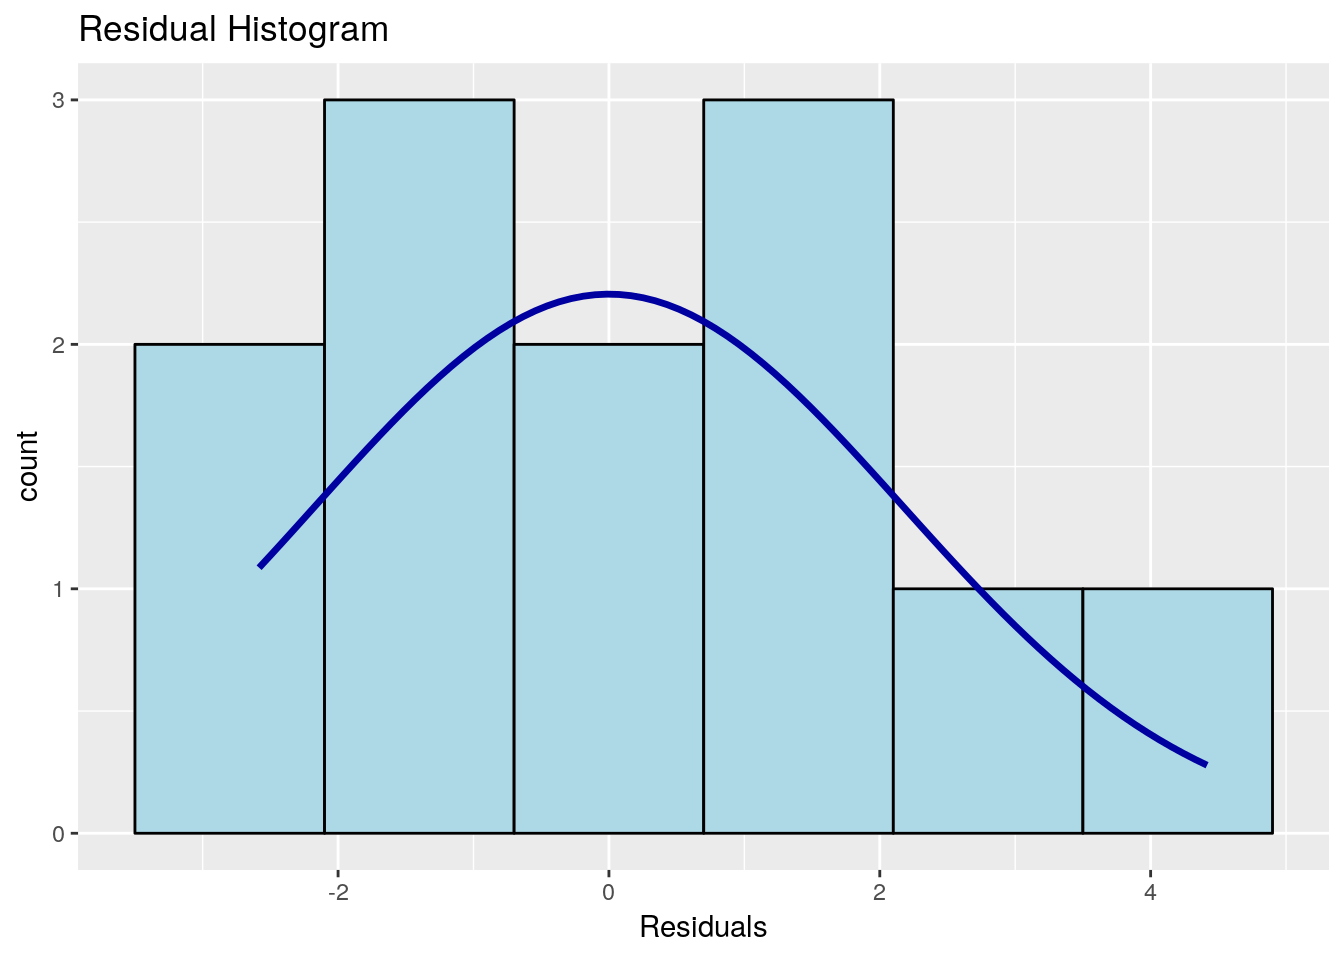
\includegraphics[width=0.2\linewidth]{hw_stat565_files/figure-latex/unnamed-chunk-22-1}
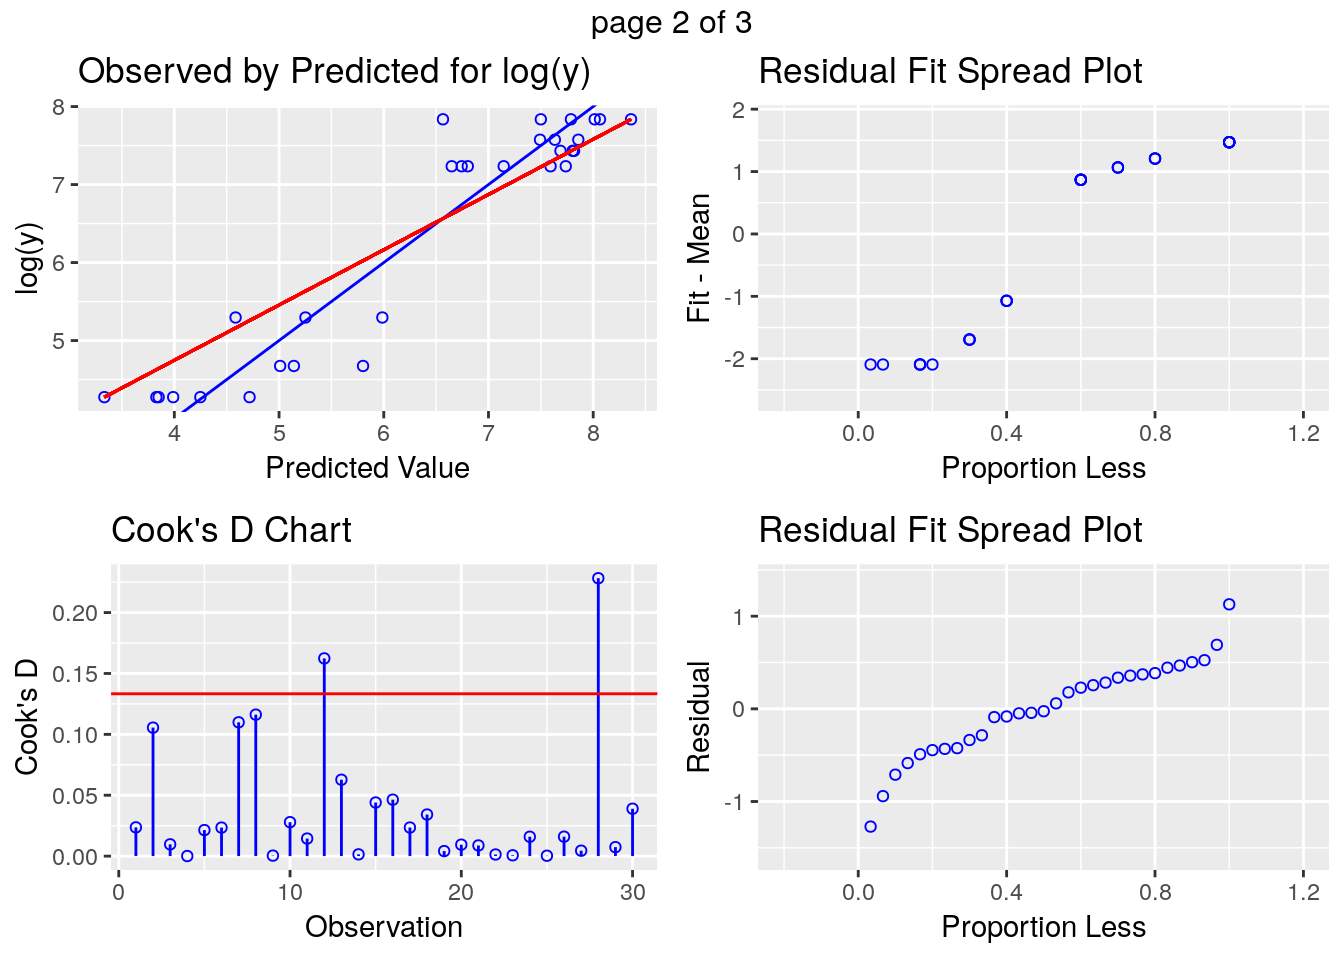
\includegraphics[width=0.2\linewidth]{hw_stat565_files/figure-latex/unnamed-chunk-22-2}
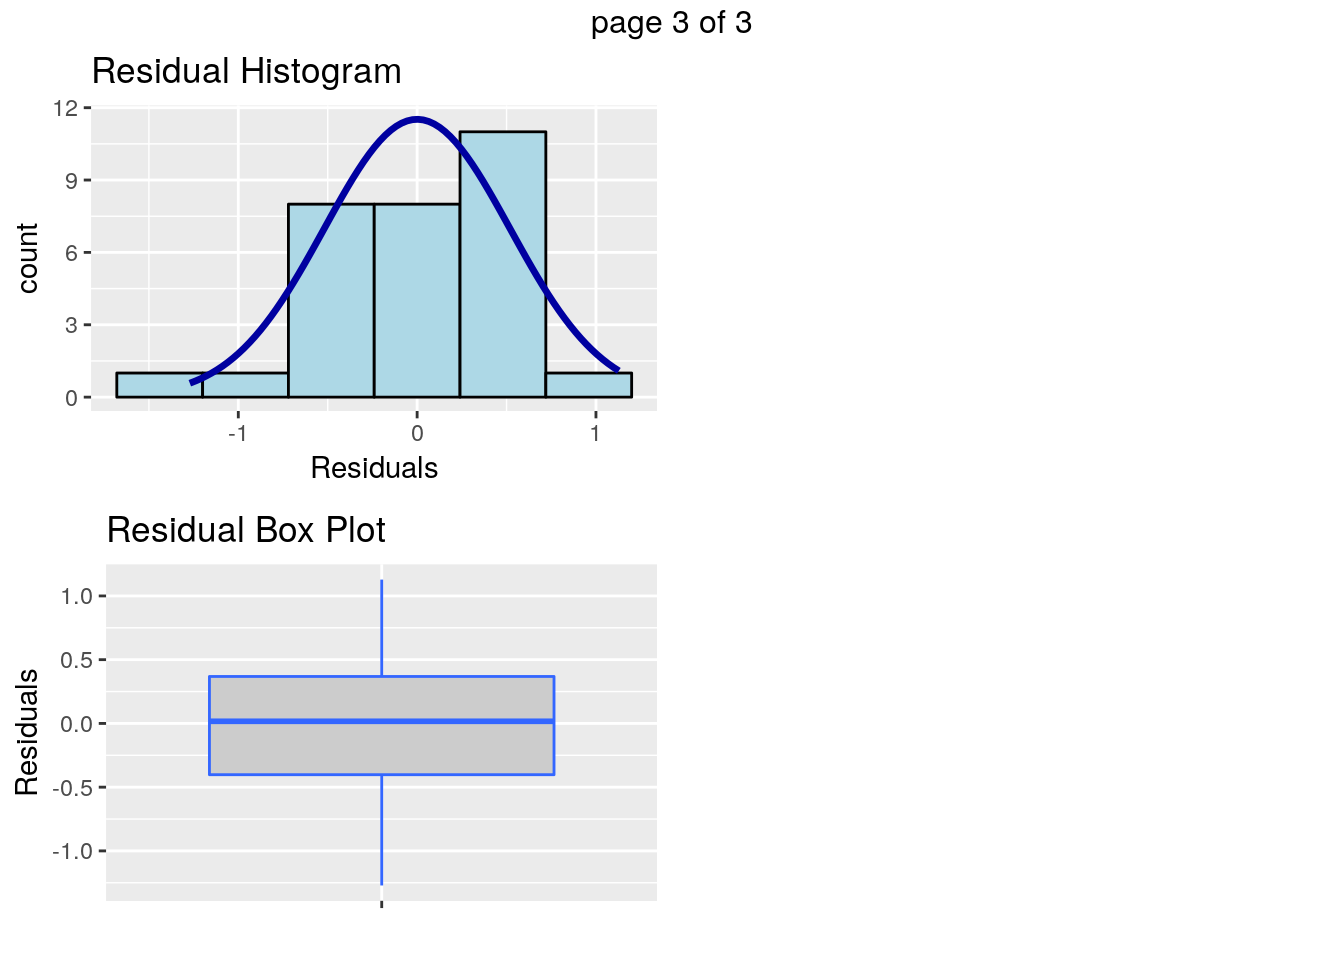
\includegraphics[width=0.2\linewidth]{hw_stat565_files/figure-latex/unnamed-chunk-22-3}
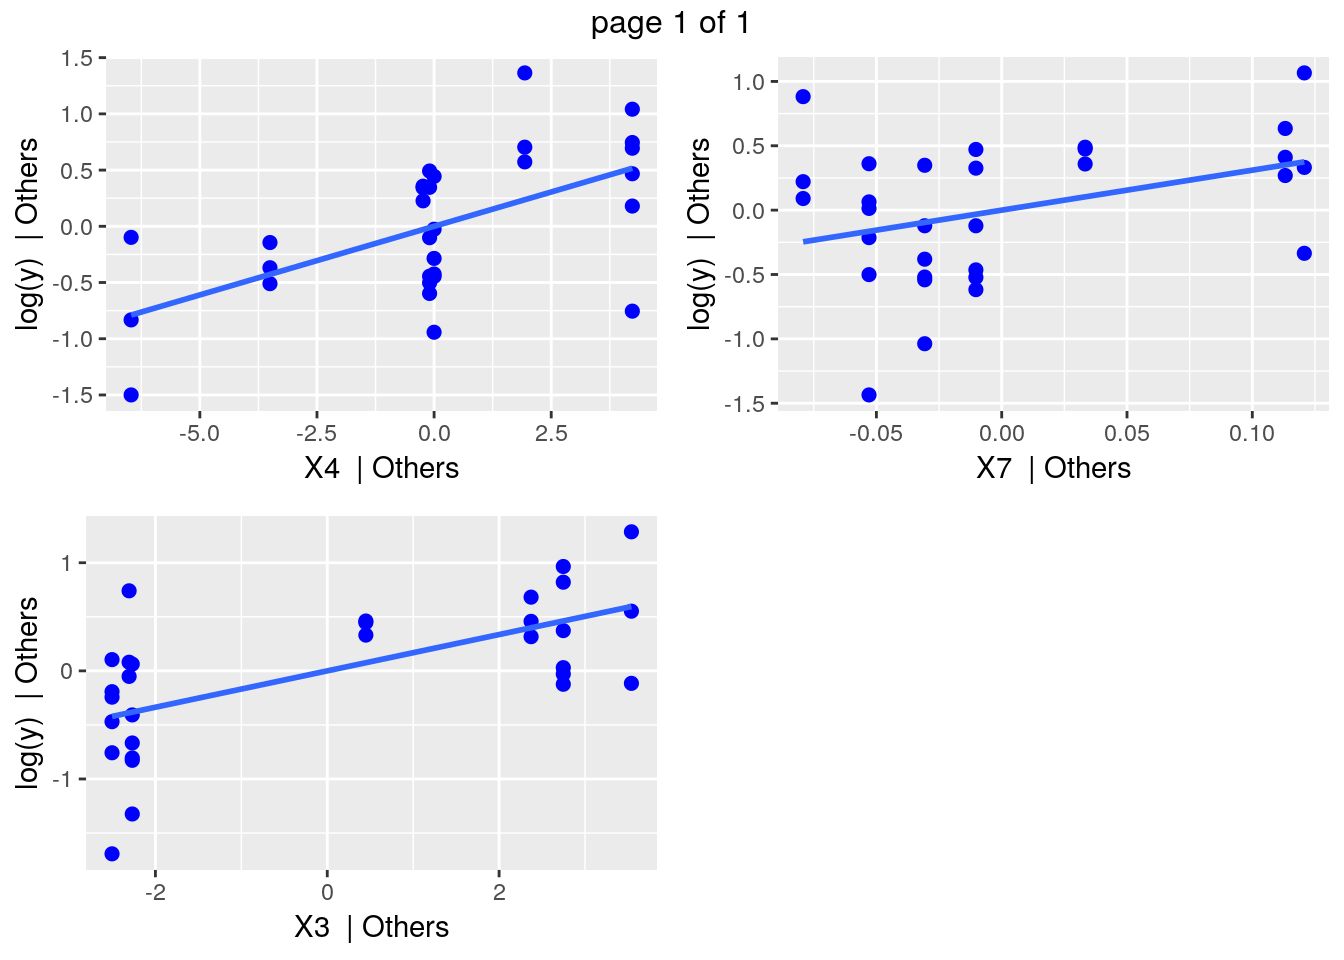
\includegraphics[width=0.2\linewidth]{hw_stat565_files/figure-latex/unnamed-chunk-22-4}
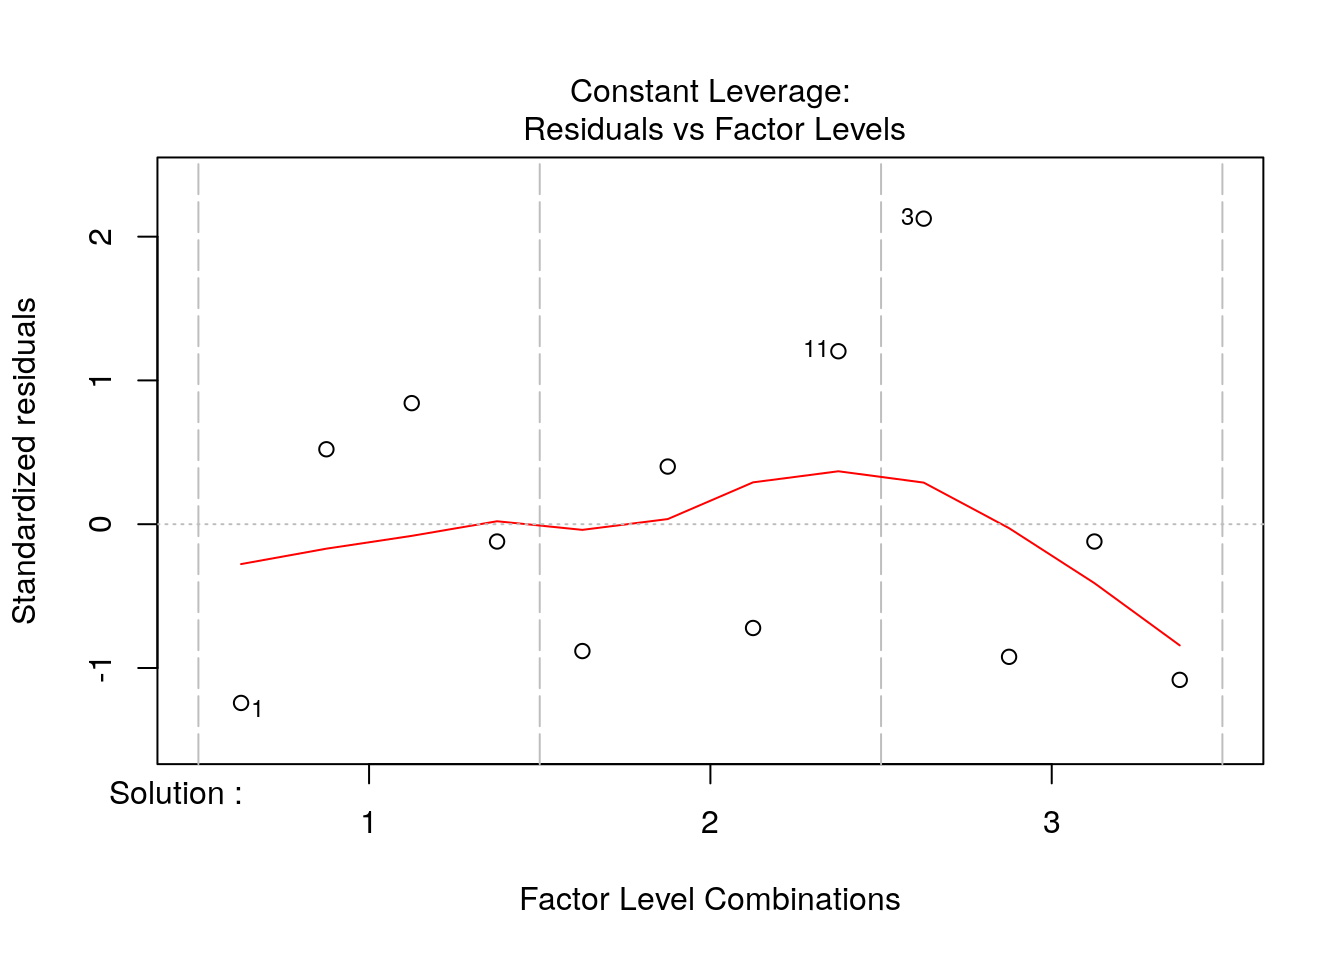
\includegraphics[width=0.2\linewidth]{hw_stat565_files/figure-latex/unnamed-chunk-22-5}
---

4.29 Consider the randomized complete block design in Problem 4.9.
Assume that the days are random. Estimate the block variance component.

\[\hat\sigma_{Blk}^2=\frac{MS_{Blk}-MS_{E}}{a}=\frac{369-8.6}{3}=120.1333\]

\begin{Shaded}
\begin{Highlighting}[]
\KeywordTok{summary}\NormalTok{(}\KeywordTok{aov}\NormalTok{(Response}\OperatorTok{~}\NormalTok{Solution}\OperatorTok{+}\KeywordTok{Error}\NormalTok{(Days), }\DataTypeTok{data=}\NormalTok{table_wash))}
\CommentTok{## }
\CommentTok{## Error: Days}
\CommentTok{##           Df Sum Sq Mean Sq F value Pr(>F)}
\CommentTok{## Residuals  3   1107     369               }
\CommentTok{## }
\CommentTok{## Error: Within}
\CommentTok{##           Df Sum Sq Mean Sq F value   Pr(>F)    }
\CommentTok{## Solution   2  703.5   351.8   40.72 0.000323 ***}
\CommentTok{## Residuals  6   51.8     8.6                     }
\CommentTok{## ---}
\CommentTok{## Signif. codes:  0 '***' 0.001 '**' 0.01 '*' 0.05 '.' 0.1 ' ' 1}
\end{Highlighting}
\end{Shaded}

\hypertarget{problem-2-4.13}{%
\subsubsection{Problem 2 (4.13)}\label{problem-2-4.13}}

A consumer products company relies on direct mail marketing pieces as a
major component of its advertising campaigns. The company has three
different designs for a new brochure and wants to evaluate their
effectiveness, as there are substantial differences in costs between the
three designs. The company decides to test the three designs by mailing
5000 samples of each to potential customers in four different regions of
the country. Since there are known regional differences in the customer
base, regions are considered as blocks. The number of responses to each
mailing is as follows.

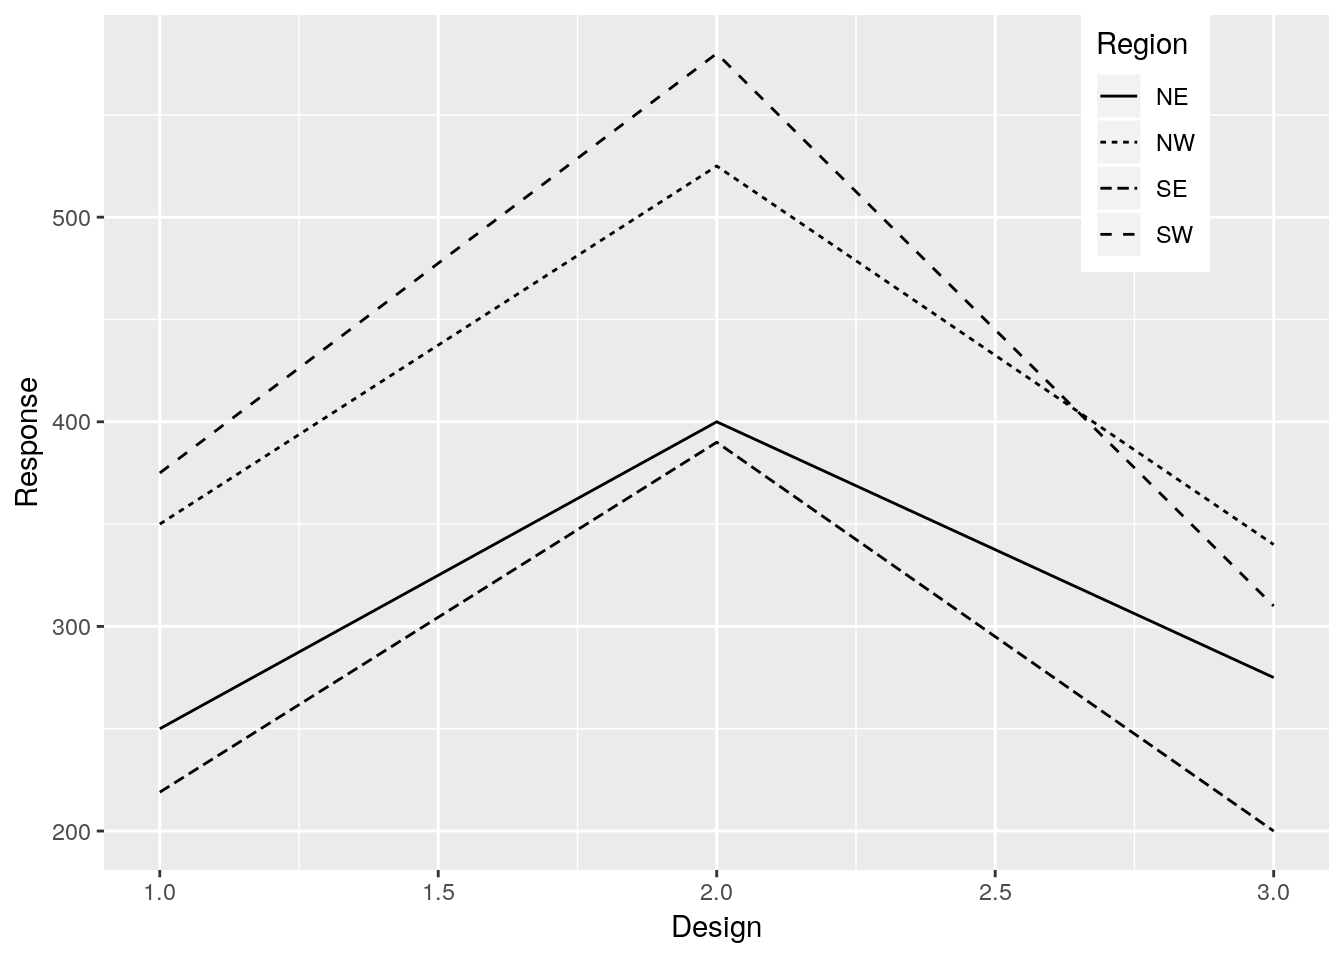
\includegraphics[width=0.45\linewidth]{hw_stat565_files/figure-latex/unnamed-chunk-24-1}

\begin{verbatim}
## Observations: 12
## Variables: 3
## $ Region   <fct> NE, NE, NE, NW, NW, NW, SE, SE, SE, SW, SW, SW
## $ Design   <fct> 1, 2, 3, 1, 2, 3, 1, 2, 3, 1, 2, 3
## $ Response <dbl> 250, 400, 275, 350, 525, 340, 219, 390, 200, 375, 580...
\end{verbatim}

\begin{enumerate}
\def\labelenumi{(\alph{enumi})}
\tightlist
\item
  Analyze the data from this experiment.
\end{enumerate}

The ANOVA for RCBD shows that both treatments of Designs and blocks of
Regions have significant effects on the average values of bacteria
growth at 0.05 significant level. The P-value for treatment is 0.00018
while it for blocks is 0.00208.

The results of estimating regression coefficients show the P-value of
Design1 and RegionNE(0.0000201), Design2(0.000173), RegionNW(0.007661),
RegionSW(0.003636) are small enough, while the P-value of
Design3(0.320563) and RegionSE(0.166470) are larger than 0.05. The
coefficients of Design1, RegionNE, Design2, RegionNW, RegionSW are
significant at 0.05 significant level. The rest are not.

\begin{Shaded}
\begin{Highlighting}[]
\NormalTok{model_mail <-}\StringTok{ }\KeywordTok{aov}\NormalTok{(Response}\OperatorTok{~}\NormalTok{Design}\OperatorTok{+}\NormalTok{Region, }\DataTypeTok{data=}\NormalTok{table_mail)}
\KeywordTok{summary}\NormalTok{(model_mail)}
\end{Highlighting}
\end{Shaded}

\begin{verbatim}
##             Df Sum Sq Mean Sq F value  Pr(>F)    
## Design       2  90755   45378   50.15 0.00018 ***
## Region       3  49036   16345   18.07 0.00208 ** 
## Residuals    6   5429     905                    
## ---
## Signif. codes:  0 '***' 0.001 '**' 0.01 '*' 0.05 '.' 0.1 ' ' 1
\end{verbatim}

\begin{Shaded}
\begin{Highlighting}[]
\KeywordTok{summary.lm}\NormalTok{(model_mail)}
\end{Highlighting}
\end{Shaded}

\begin{verbatim}
## 
## Call:
## aov(formula = Response ~ Design + Region, data = table_mail)
## 
## Residuals:
##     Min      1Q  Median      3Q     Max 
## -41.750  -3.354  -1.000   5.188  36.583 
## 
## Coefficients:
##             Estimate Std. Error t value Pr(>|t|)    
## (Intercept)   255.67      21.27  12.020 2.01e-05 ***
## Design2       175.25      21.27   8.239 0.000173 ***
## Design3       -17.25      21.27  -0.811 0.448327    
## RegionNW       96.67      24.56   3.936 0.007661 ** 
## RegionSE      -38.67      24.56  -1.574 0.166470    
## RegionSW      113.33      24.56   4.615 0.003636 ** 
## ---
## Signif. codes:  0 '***' 0.001 '**' 0.01 '*' 0.05 '.' 0.1 ' ' 1
## 
## Residual standard error: 30.08 on 6 degrees of freedom
## Multiple R-squared:  0.9626, Adjusted R-squared:  0.9315 
## F-statistic:  30.9 on 5 and 6 DF,  p-value: 0.0003285
\end{verbatim}

\begin{center}\rule{0.5\linewidth}{\linethickness}\end{center}

\begin{enumerate}
\def\labelenumi{(\alph{enumi})}
\setcounter{enumi}{1}
\tightlist
\item
  Use the Fisher LSD method to make comparisons among the three designs
  to determine specifically which designs differ in the mean response
  rate.
\end{enumerate}

The plot of LSD test shows the average response value for Design2 has a
different interval with that for other designs. The LSD test using
``pairw.anova'' also shows the average response values for Design2 are
significant different with Design1(P-value=0.01108) and
Design3(P-value=0.00673) at 0.05 significant level, while there is not
significant difference between the average response value for Design1
and Design3(P-value=0.76098) at 0.05 significant level.

\begin{Shaded}
\begin{Highlighting}[]
\KeywordTok{plot}\NormalTok{(}\KeywordTok{LSD.test}\NormalTok{(model_mail, }\DataTypeTok{trt=}\StringTok{"Design"}\NormalTok{,}\DataTypeTok{alpha =} \FloatTok{0.05}\NormalTok{,}\DataTypeTok{p.adj=}\StringTok{"bonferroni"}\NormalTok{))}
\end{Highlighting}
\end{Shaded}

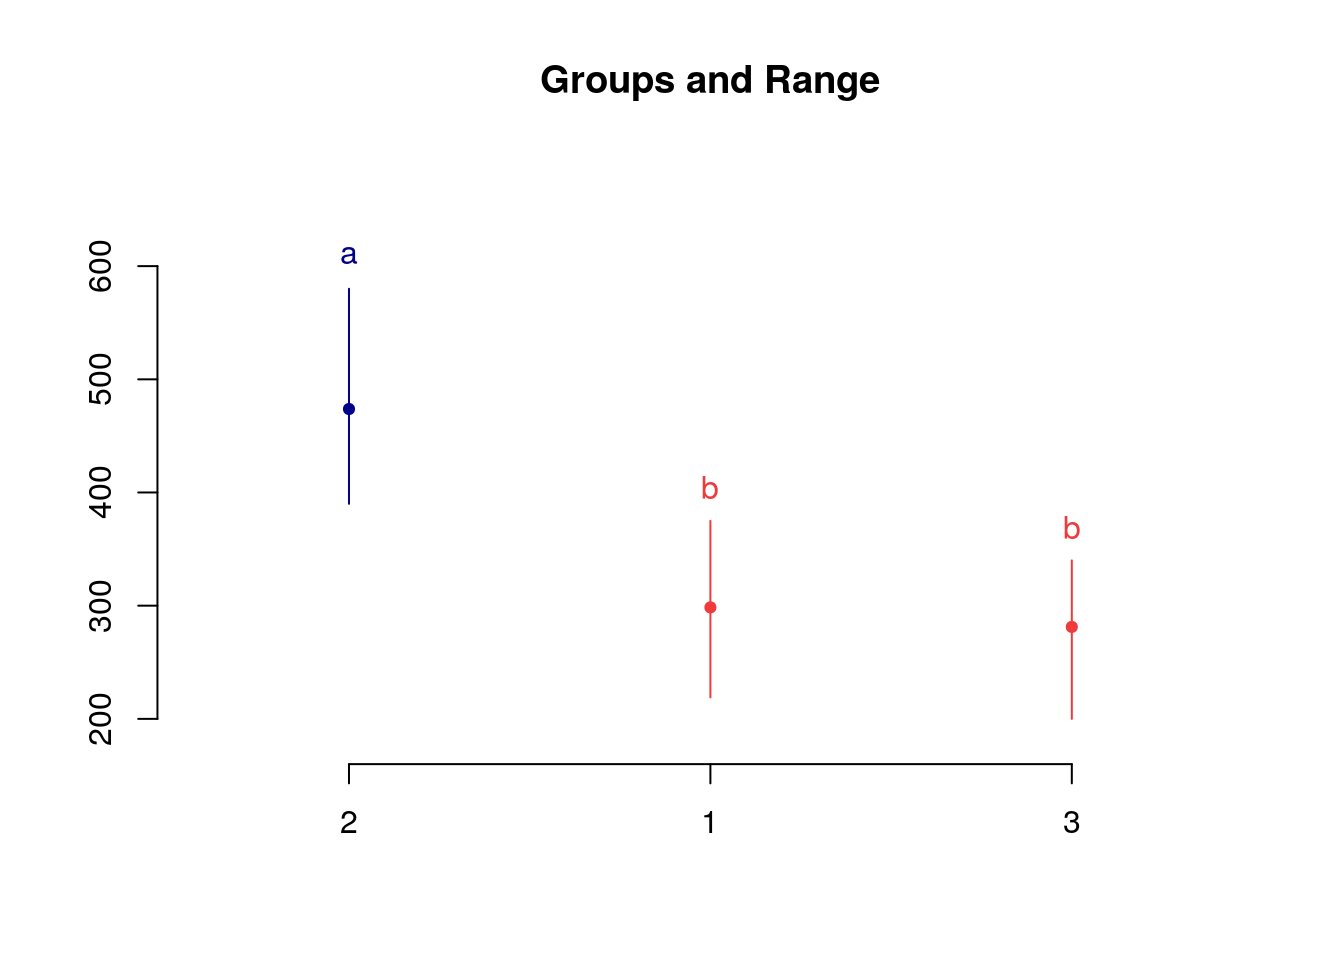
\includegraphics[width=0.24\linewidth]{hw_stat565_files/figure-latex/unnamed-chunk-26-1}

\begin{Shaded}
\begin{Highlighting}[]
\KeywordTok{pairw.anova}\NormalTok{(table_mail}\OperatorTok{$}\NormalTok{Response,table_mail}\OperatorTok{$}\NormalTok{Design, }\DataTypeTok{conf.level =} \FloatTok{0.95}\NormalTok{, }\DataTypeTok{method =} \StringTok{"lsd"}\NormalTok{, }\DataTypeTok{MSE =} \OtherTok{NULL}\NormalTok{, }\DataTypeTok{df.err =} \OtherTok{NULL}\NormalTok{, }\DataTypeTok{control =} \OtherTok{NULL}\NormalTok{)}
\CommentTok{## }
\CommentTok{## 95% LSD confidence intervals }
\CommentTok{## }
\CommentTok{##               LSD    Diff      Lower     Upper  Decision Adj. p-value}
\CommentTok{## mu1-mu2 124.43521 -175.25 -299.68521 -50.81479 Reject H0      0.01108}
\CommentTok{## mu1-mu3 124.43521   17.25 -107.18521 141.68521    FTR H0      0.76098}
\CommentTok{## mu2-mu3 124.43521   192.5   68.06479 316.93521 Reject H0      0.00673}
\end{Highlighting}
\end{Shaded}

\begin{center}\rule{0.5\linewidth}{\linethickness}\end{center}

\begin{enumerate}
\def\labelenumi{(\alph{enumi})}
\setcounter{enumi}{2}
\tightlist
\item
  Analyze the residuals from this experiment.
\end{enumerate}

\begin{itemize}
\tightlist
\item
  Model adequacy Checking
\end{itemize}

The normality test and histogram of residuals show a violation of
normality. The QQ plot of residuals shows a sharp upward and downward
curve at both extremes, indicating that the tails of this distribution
are too light for it to be considered normal. The variance of \(y\)
seems be proportional to \(x\) which implies \(y\) may be a Poisson
random variable in a simple linear regression model and its variance is
equal to the mean. We could regress \(y′=\sqrt y\) against \(x\) since
the variance of the square root of a Poisson random variable is
independent of the mean.

\begin{itemize}
\tightlist
\item
  After transformation
\end{itemize}

The violation of normality in QQ plot and histogram are not obvious as
before. The residuals versus fitted values and studentized residuals
don't show strong violation of zero mean and constant variance
assumptions. There is not serious outlier and leverage data points. The
residuals versus observation number shows the residuals are independent
with each other.

The ANOVA for RCBD shows simular results. Moreover, MSE after
transformation(0.502) is much smaller than before(905). The P-value is
smaller too (0.000106 for treatment, 0.000986 for blocks).

The results of estimating regression coefficients are simular. The
P-value of Design1 and RegionNE(0.000006), Design2(0.000105),
RegionNW(0.004490), RegionSW(0.002479) are smaller, while the P-value of
Design3(0.376944) and RegionSE(0.076721) are still larger than 0.05. The
coefficients of Design1, RegionNE, Design2, RegionNW, RegionSW are
significant at 0.05 significant level. The rest are not.

The results of paried test are same. The plot of LSD test shows the
average response value for Design2 has a different interval with that
for other designs. The LSD test using ``pairw.anova'' also shows the
average response values for Design2 are significant different with
Design1(P-value=0.01333) and Design3(P-value=0.00792) at 0.05
significant level, while there is not significant difference between
Design1 and Design3(P-value=0.7525) at 0.05 significant level.

\begin{Shaded}
\begin{Highlighting}[]
\KeywordTok{ols_test_normality}\NormalTok{(}\KeywordTok{lm}\NormalTok{(Response}\OperatorTok{~}\NormalTok{Design}\OperatorTok{+}\NormalTok{Region, }\DataTypeTok{data=}\NormalTok{table_mail))}
\CommentTok{## -----------------------------------------------}
\CommentTok{##        Test             Statistic       pvalue  }
\CommentTok{## -----------------------------------------------}
\CommentTok{## Shapiro-Wilk              0.8887         0.1133 }
\CommentTok{## Kolmogorov-Smirnov        0.2327         0.4654 }
\CommentTok{## Cramer-von Mises          0.875          0.0039 }
\CommentTok{## Anderson-Darling          0.7294         0.0414 }
\CommentTok{## -----------------------------------------------}
\KeywordTok{ols_test_normality}\NormalTok{(}\KeywordTok{lm}\NormalTok{(}\KeywordTok{sqrt}\NormalTok{(Response)}\OperatorTok{~}\NormalTok{Design}\OperatorTok{+}\NormalTok{Region, }\DataTypeTok{data=}\NormalTok{table_mail))}
\CommentTok{## -----------------------------------------------}
\CommentTok{##        Test             Statistic       pvalue  }
\CommentTok{## -----------------------------------------------}
\CommentTok{## Shapiro-Wilk              0.9865         0.9981 }
\CommentTok{## Kolmogorov-Smirnov        0.1116         0.9941 }
\CommentTok{## Cramer-von Mises          1.3217          2e-04 }
\CommentTok{## Anderson-Darling          0.1502         0.9464 }
\CommentTok{## -----------------------------------------------}
\KeywordTok{ols_plot_resid_hist}\NormalTok{(}\KeywordTok{lm}\NormalTok{(Response}\OperatorTok{~}\NormalTok{Design}\OperatorTok{+}\NormalTok{Region, }\DataTypeTok{data=}\NormalTok{table_mail))}
\KeywordTok{plot}\NormalTok{(model_mail)}
\KeywordTok{ols_plot_resid_hist}\NormalTok{(}\KeywordTok{lm}\NormalTok{(}\KeywordTok{sqrt}\NormalTok{(Response)}\OperatorTok{~}\NormalTok{Design}\OperatorTok{+}\NormalTok{Region, }\DataTypeTok{data=}\NormalTok{table_mail))}
\KeywordTok{plot}\NormalTok{(}\KeywordTok{lm}\NormalTok{(}\KeywordTok{sqrt}\NormalTok{(Response)}\OperatorTok{~}\NormalTok{Design}\OperatorTok{+}\NormalTok{Region, }\DataTypeTok{data=}\NormalTok{table_mail))}
\end{Highlighting}
\end{Shaded}

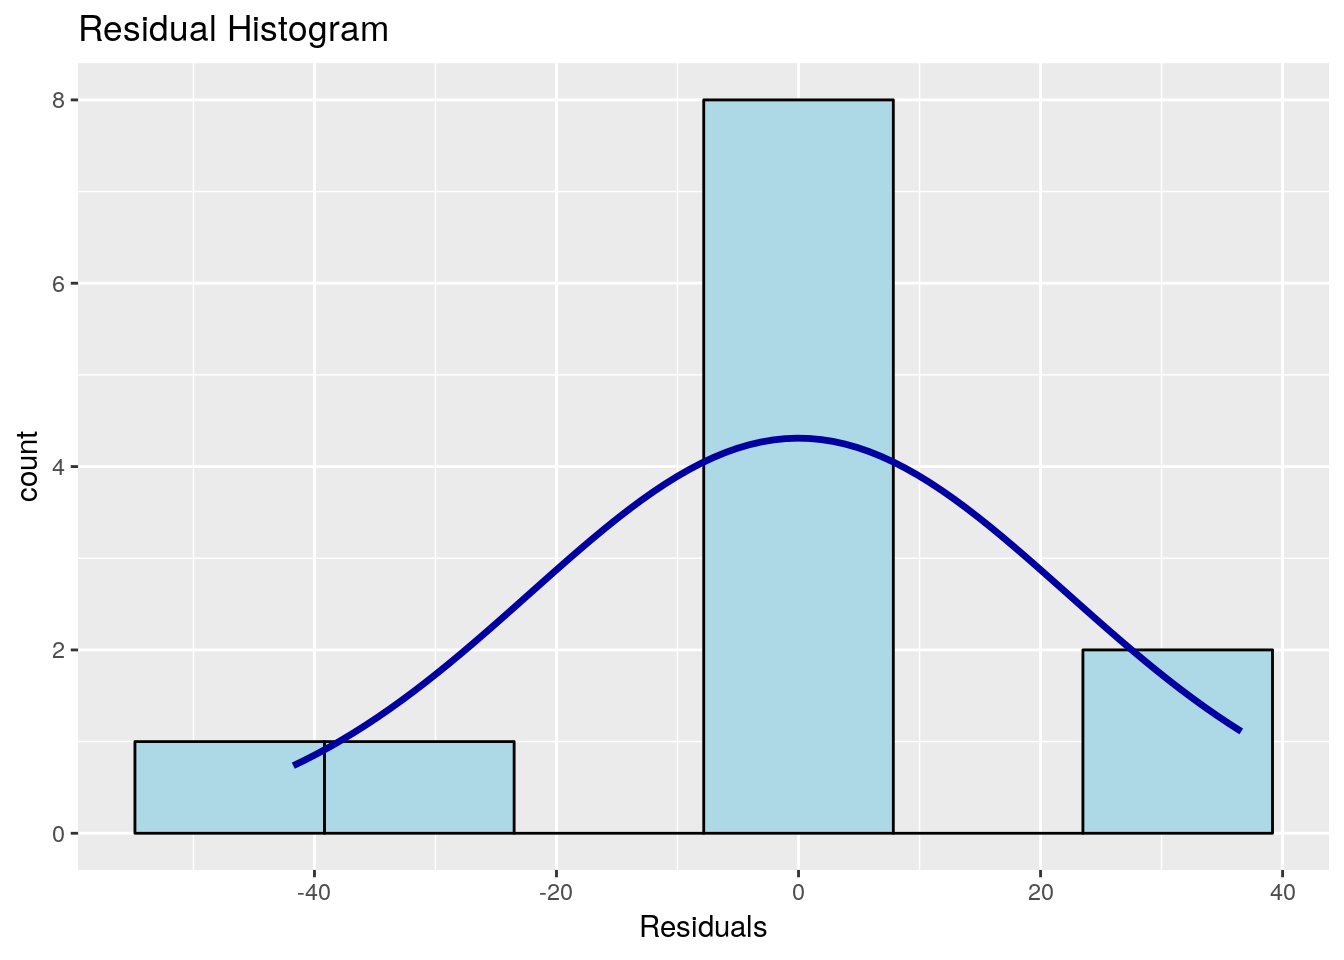
\includegraphics[width=0.2\linewidth]{hw_stat565_files/figure-latex/unnamed-chunk-27-1}
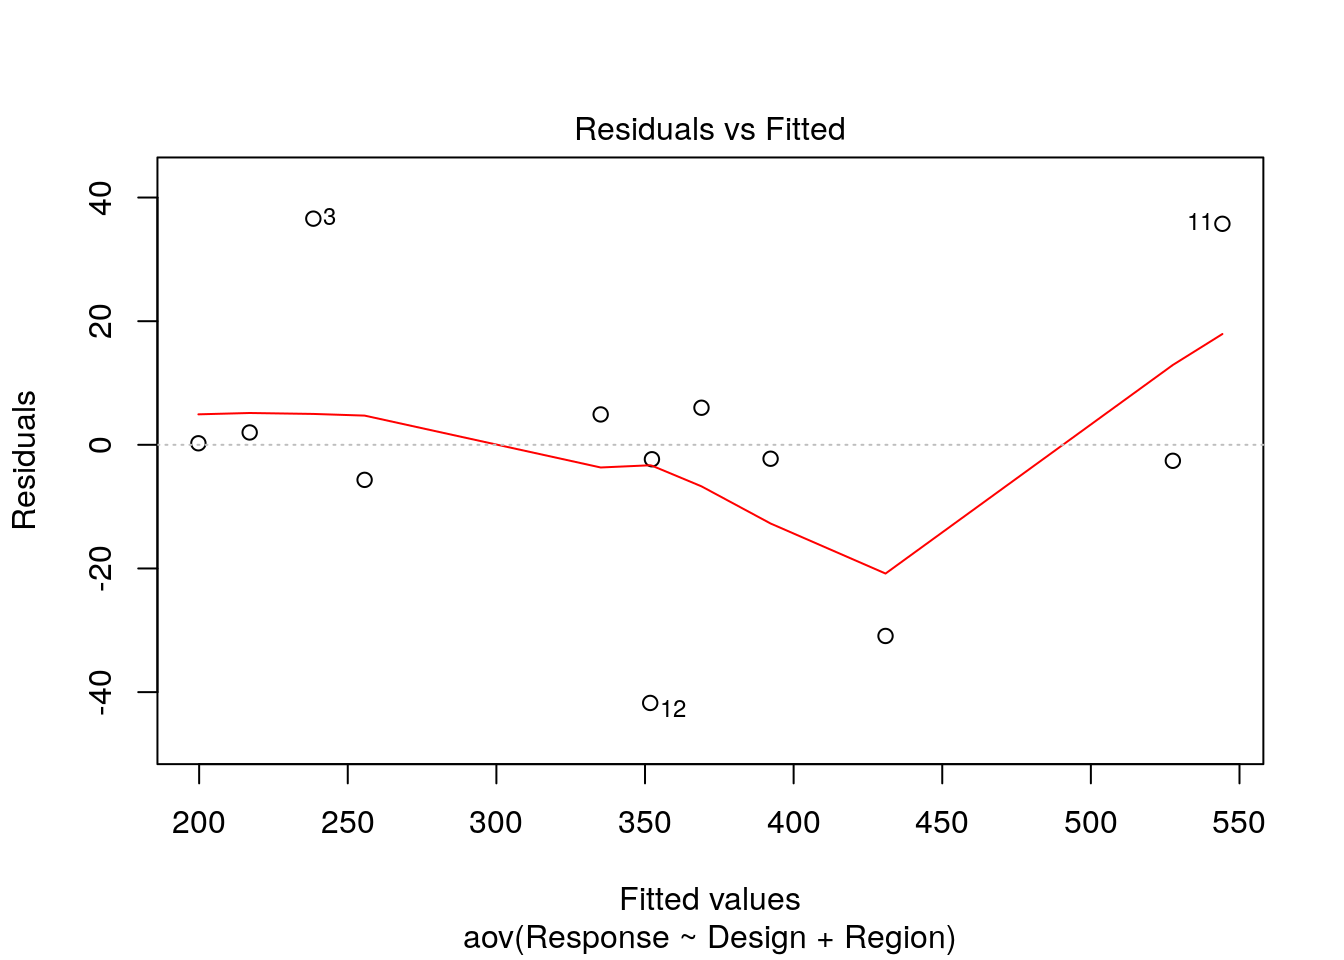
\includegraphics[width=0.2\linewidth]{hw_stat565_files/figure-latex/unnamed-chunk-27-2}
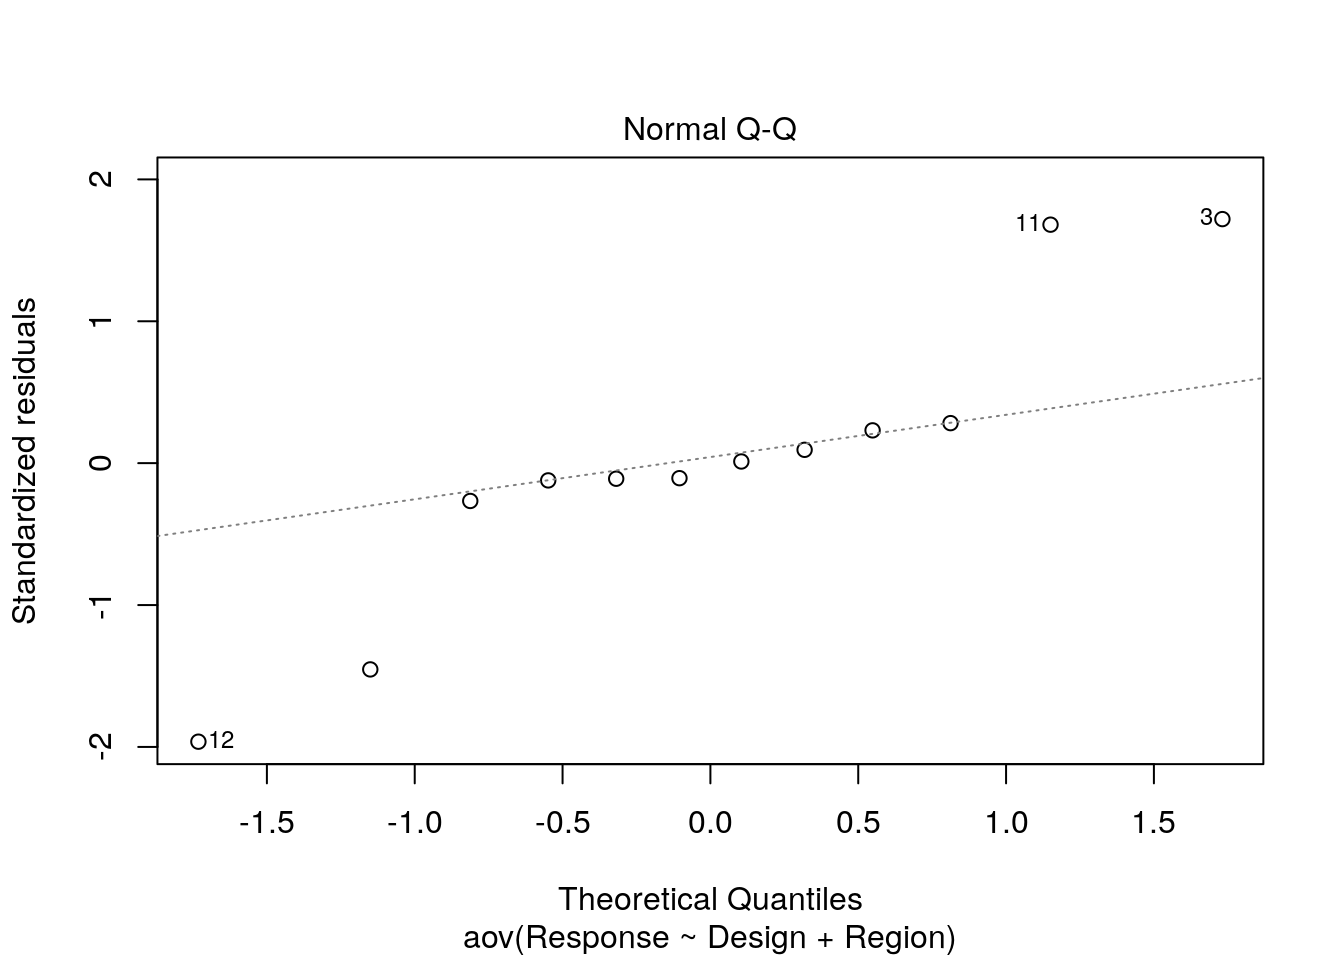
\includegraphics[width=0.2\linewidth]{hw_stat565_files/figure-latex/unnamed-chunk-27-3}
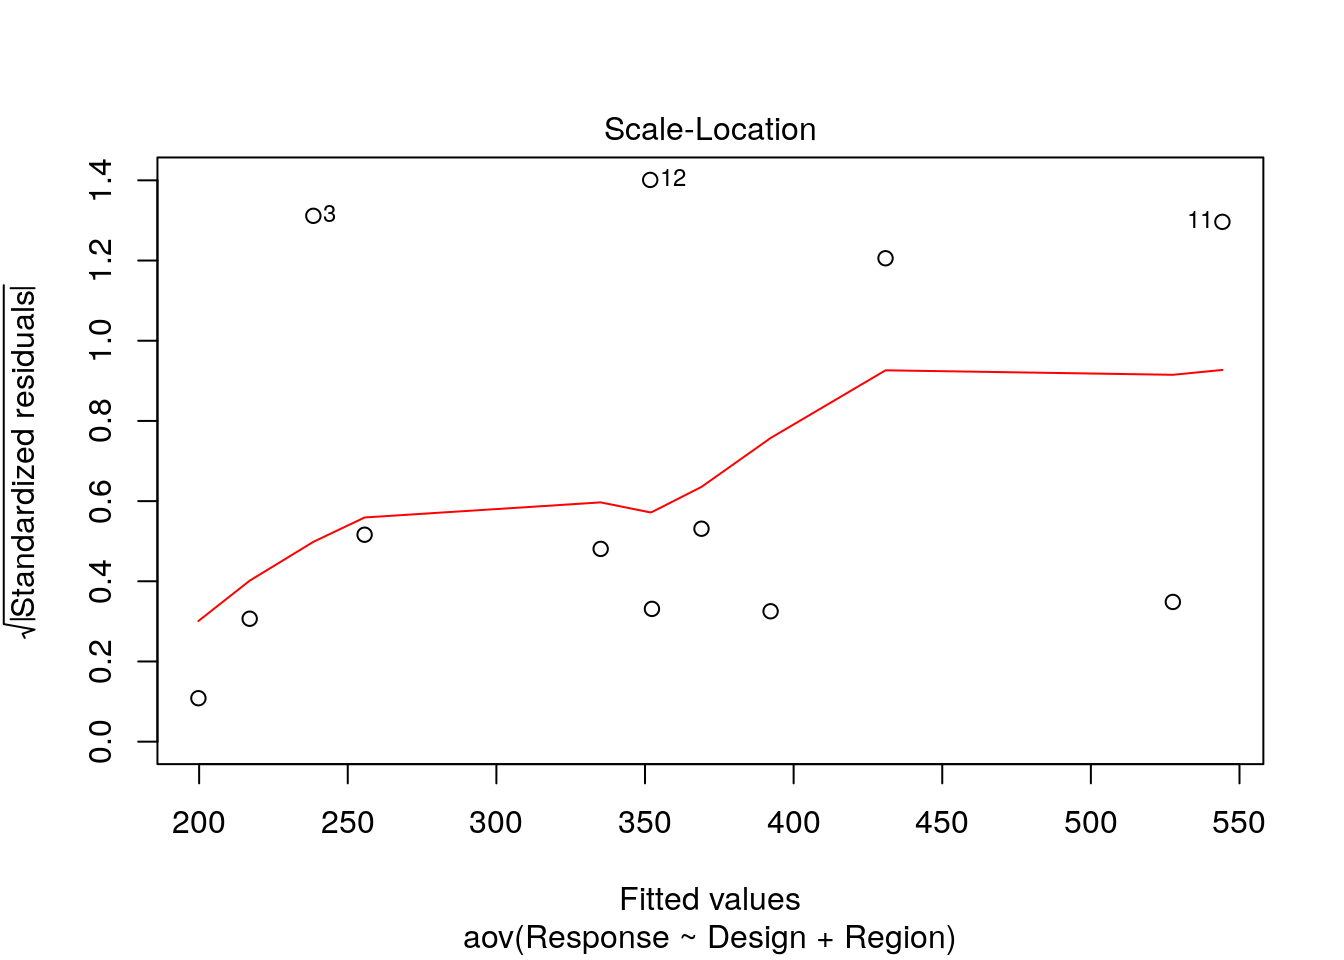
\includegraphics[width=0.2\linewidth]{hw_stat565_files/figure-latex/unnamed-chunk-27-4}
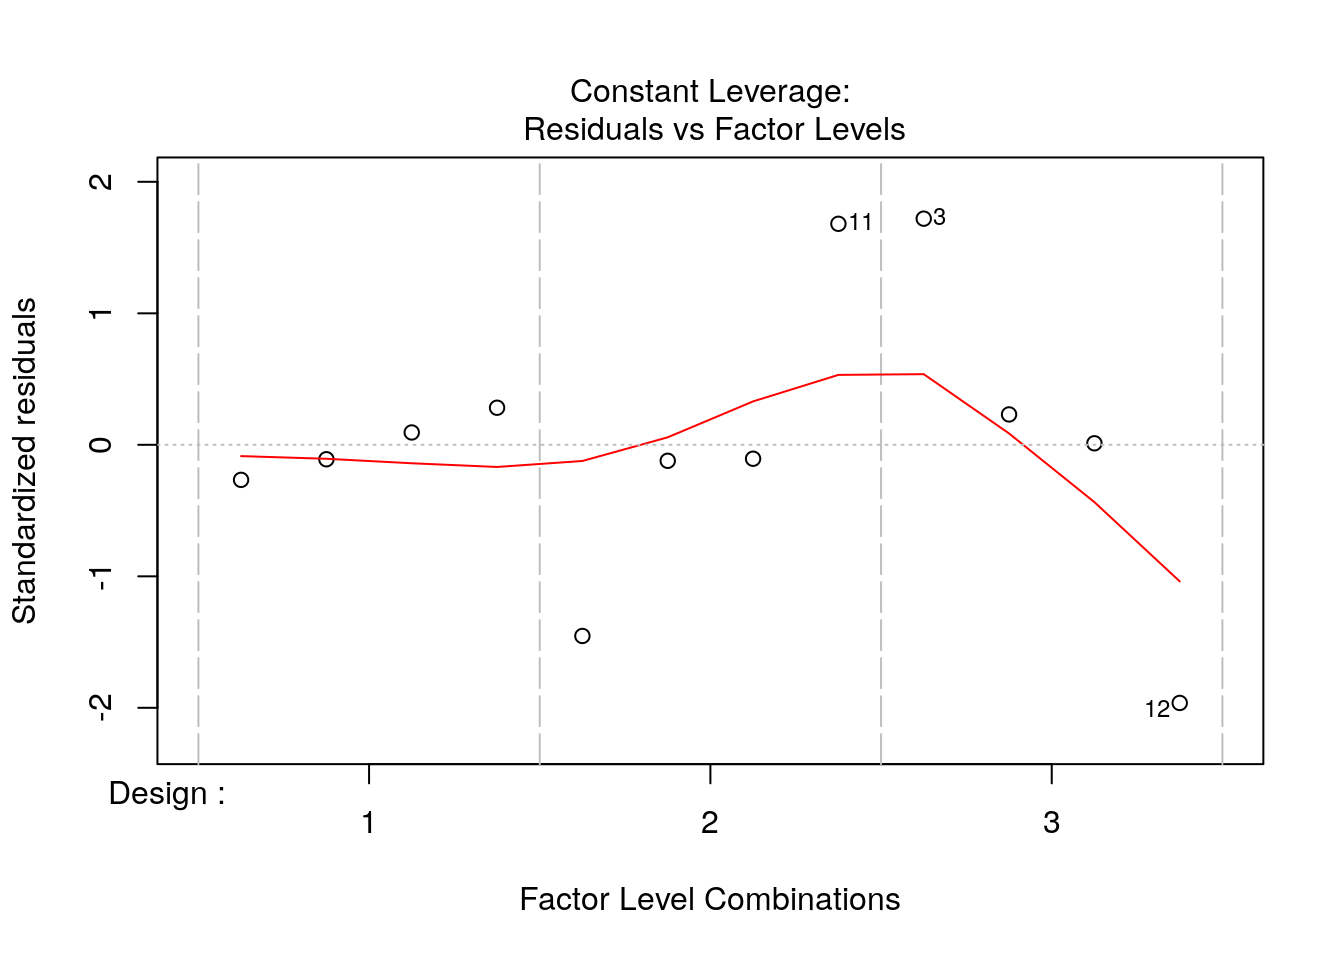
\includegraphics[width=0.2\linewidth]{hw_stat565_files/figure-latex/unnamed-chunk-27-5}
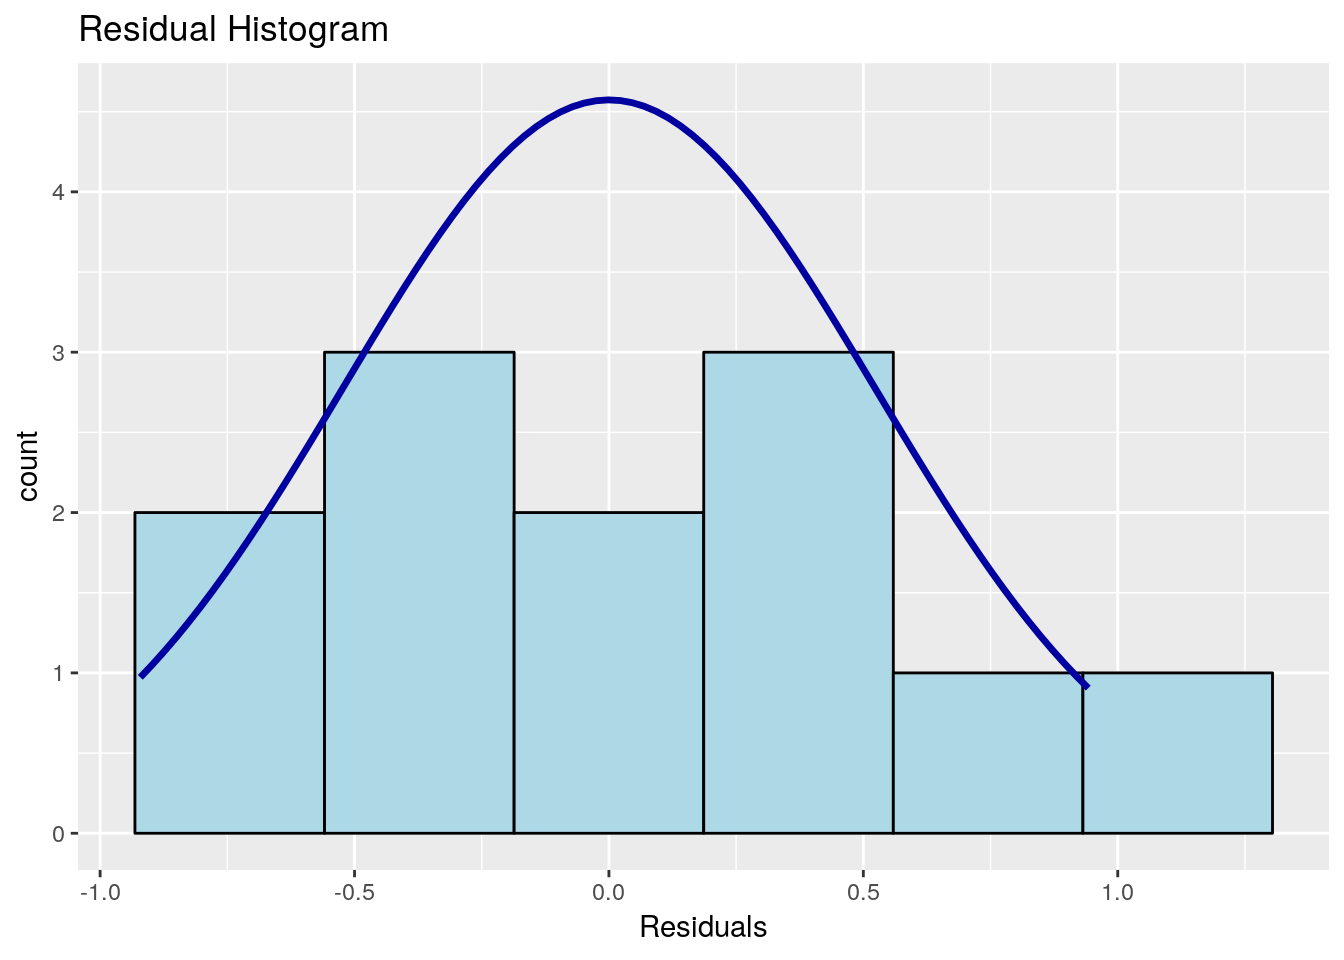
\includegraphics[width=0.2\linewidth]{hw_stat565_files/figure-latex/unnamed-chunk-27-6}
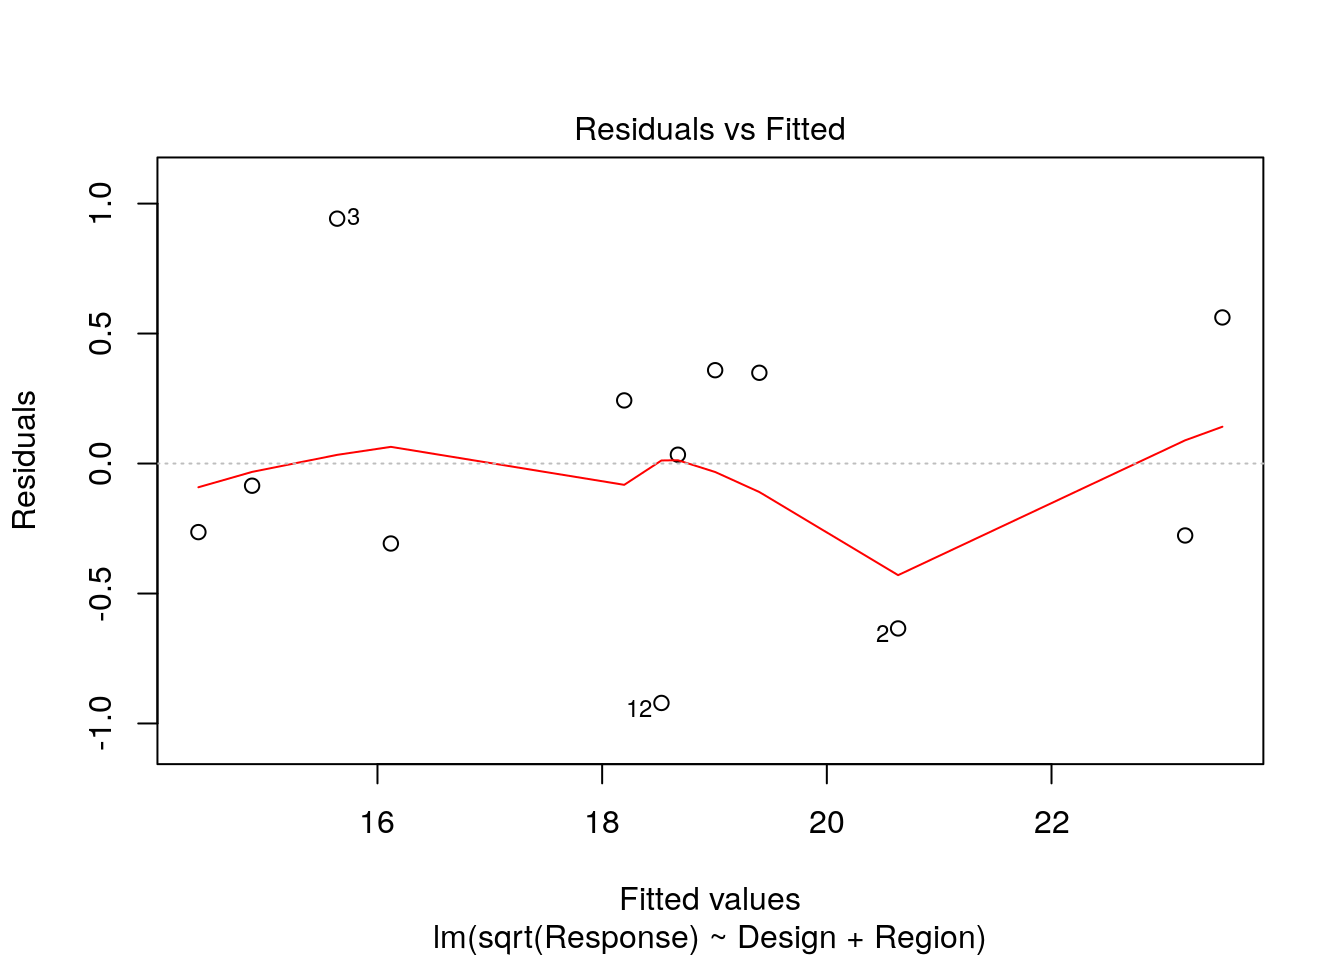
\includegraphics[width=0.2\linewidth]{hw_stat565_files/figure-latex/unnamed-chunk-27-7}
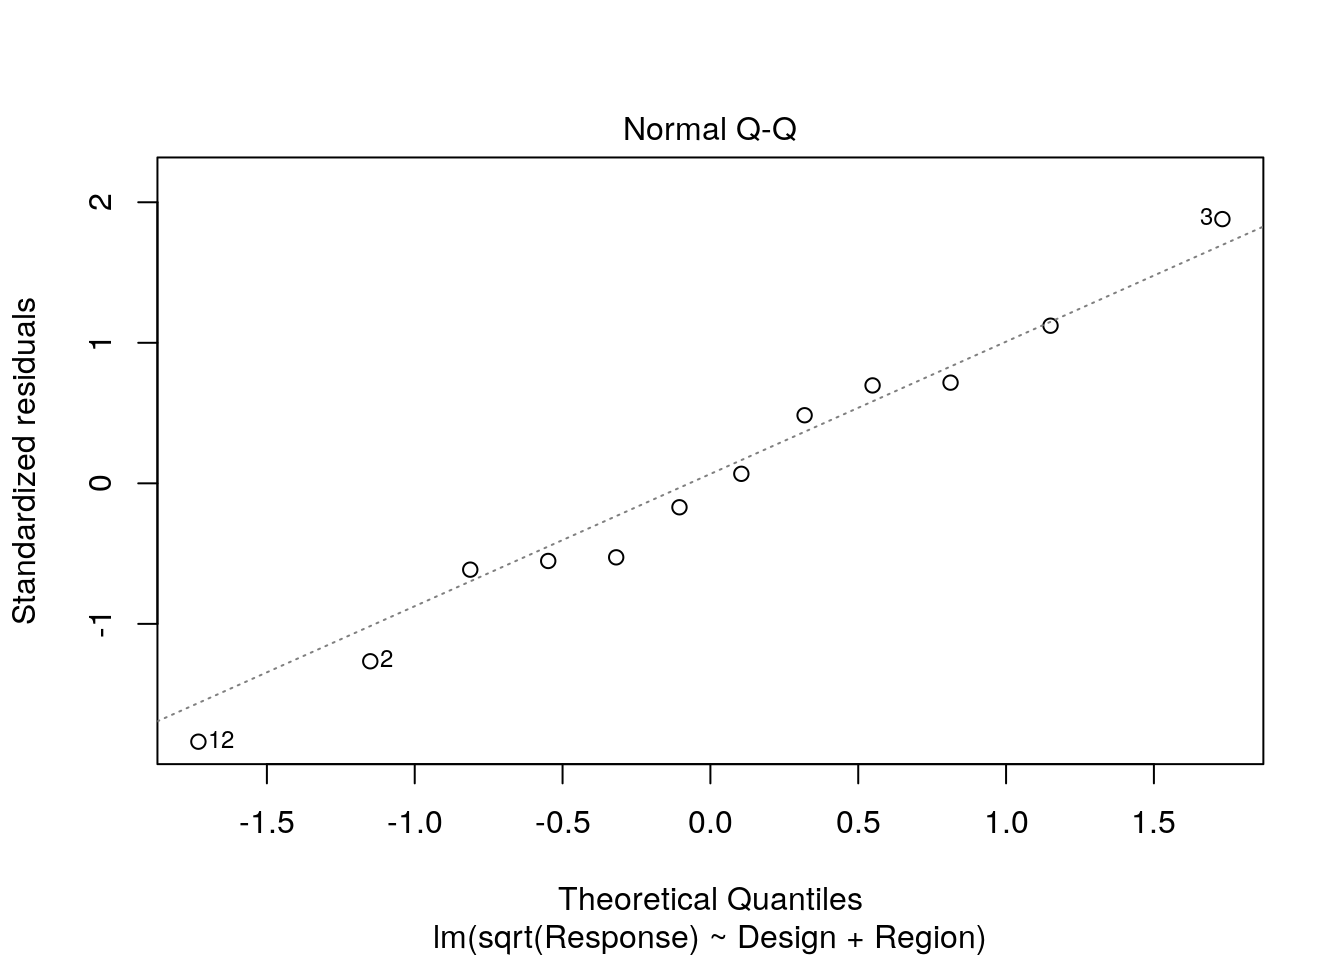
\includegraphics[width=0.2\linewidth]{hw_stat565_files/figure-latex/unnamed-chunk-27-8}
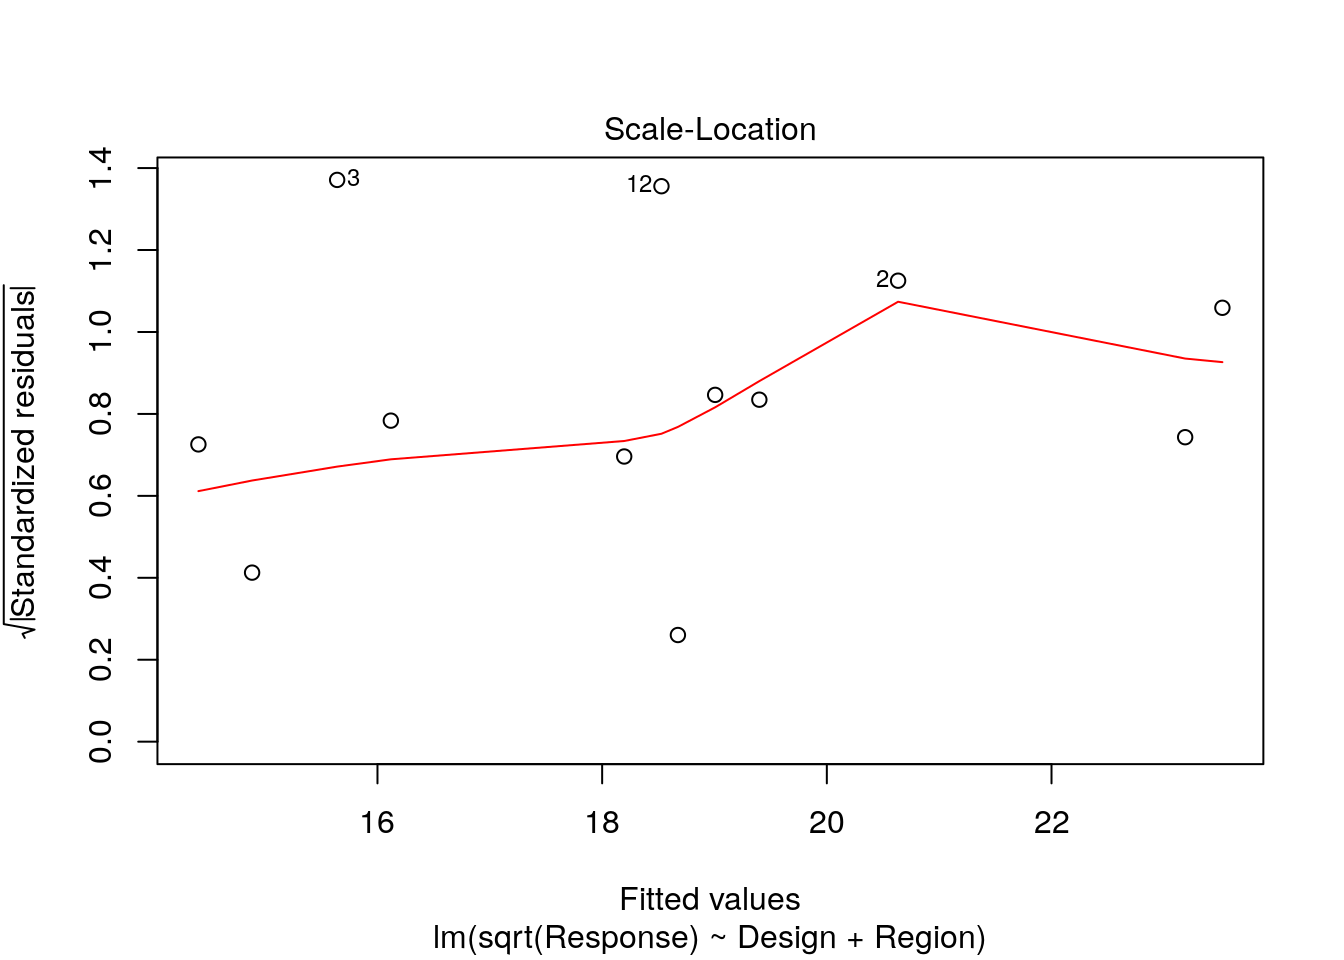
\includegraphics[width=0.2\linewidth]{hw_stat565_files/figure-latex/unnamed-chunk-27-9}
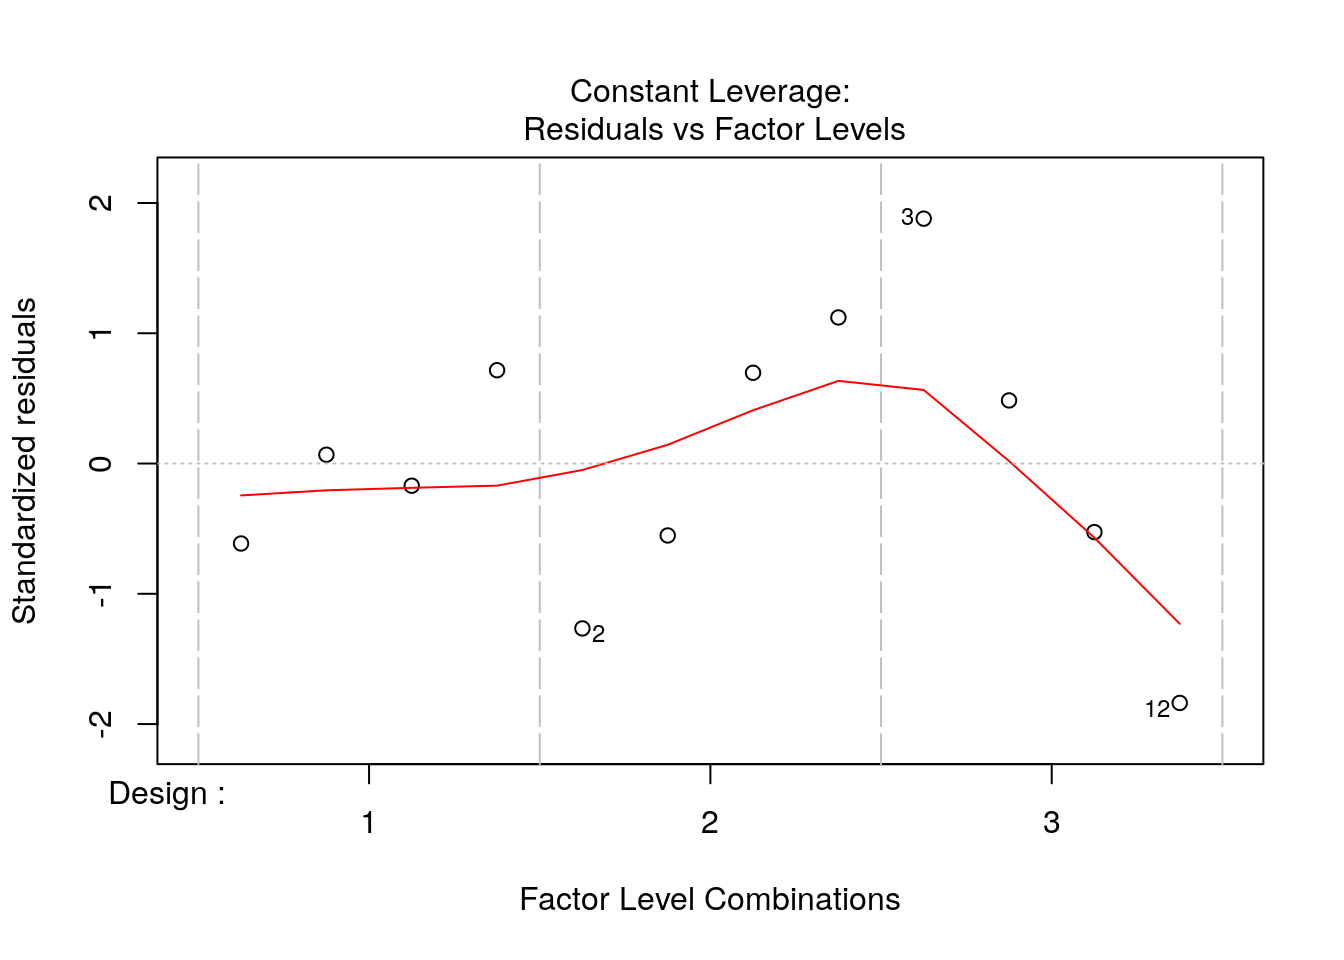
\includegraphics[width=0.2\linewidth]{hw_stat565_files/figure-latex/unnamed-chunk-27-10}

\begin{Shaded}
\begin{Highlighting}[]
\NormalTok{model_mail_sqrt <-}\StringTok{ }\KeywordTok{aov}\NormalTok{(}\KeywordTok{sqrt}\NormalTok{(Response)}\OperatorTok{~}\NormalTok{Design}\OperatorTok{+}\NormalTok{Region, }\DataTypeTok{data=}\NormalTok{table_mail)}
\KeywordTok{summary}\NormalTok{(model_mail_sqrt)}
\end{Highlighting}
\end{Shaded}

\begin{verbatim}
##             Df Sum Sq Mean Sq F value   Pr(>F)    
## Design       2  60.73  30.367   60.47 0.000106 ***
## Region       3  35.89  11.964   23.82 0.000986 ***
## Residuals    6   3.01   0.502                     
## ---
## Signif. codes:  0 '***' 0.001 '**' 0.01 '*' 0.05 '.' 0.1 ' ' 1
\end{verbatim}

\begin{Shaded}
\begin{Highlighting}[]
\KeywordTok{summary.lm}\NormalTok{(model_mail_sqrt)}
\end{Highlighting}
\end{Shaded}

\begin{verbatim}
## 
## Call:
## aov(formula = sqrt(Response) ~ Design + Region, data = table_mail)
## 
## Residuals:
##      Min       1Q   Median       3Q      Max 
## -0.92104 -0.28449 -0.02568  0.35161  0.94207 
## 
## Coefficients:
##             Estimate Std. Error t value Pr(>|t|)    
## (Intercept)  16.1191     0.5011  32.168    6e-08 ***
## Design2       4.5153     0.5011   9.011 0.000105 ***
## Design3      -0.4780     0.5011  -0.954 0.376944    
## RegionNW      2.5552     0.5786   4.416 0.004490 ** 
## RegionSE     -1.2351     0.5786  -2.135 0.076721 .  
## RegionSW      2.8868     0.5786   4.989 0.002479 ** 
## ---
## Signif. codes:  0 '***' 0.001 '**' 0.01 '*' 0.05 '.' 0.1 ' ' 1
## 
## Residual standard error: 0.7087 on 6 degrees of freedom
## Multiple R-squared:  0.9698, Adjusted R-squared:  0.9446 
## F-statistic: 38.48 on 5 and 6 DF,  p-value: 0.0001754
\end{verbatim}

\begin{Shaded}
\begin{Highlighting}[]
\CommentTok{# plot(LSD.test(model_mail_sqrt, trt="Design",alpha = 0.05,p.adj="bonferroni"))}
\KeywordTok{pairw.anova}\NormalTok{(}\KeywordTok{sqrt}\NormalTok{(table_mail}\OperatorTok{$}\NormalTok{Response),table_mail}\OperatorTok{$}\NormalTok{Design, }\DataTypeTok{conf.level =} \FloatTok{0.95}\NormalTok{, }\DataTypeTok{method =} \StringTok{"lsd"}\NormalTok{)}
\CommentTok{## }
\CommentTok{## 95% LSD confidence intervals }
\CommentTok{## }
\CommentTok{##             LSD     Diff    Lower    Upper  Decision Adj. p-value}
\CommentTok{## mu1-mu2 3.32573 -4.51531 -7.84104 -1.18958 Reject H0      0.01333}
\CommentTok{## mu1-mu3 3.32573  0.47802 -2.84771  3.80375    FTR H0       0.7525}
\CommentTok{## mu2-mu3 3.32573  4.99333   1.6676  8.31906 Reject H0      0.00792}
\end{Highlighting}
\end{Shaded}

\hypertarget{problem-3-2}{%
\subsubsection{Problem 3}\label{problem-3-2}}

\(y_{ijkl}=μ+τ_i+α_{j(l)}+β_k+δ_l+ε_{ijkl}\) for \(i,j,k =1,…,p\) ;
\(l=1,…,n\); \(ε_{ijkl}\sim iid N(0,σ^2 )\) Derive the parameter
estimates from the least squares method using the constrains
\(\sum_i\hat\tau_i=0;\ \sum_j\hat\alpha_{j(l)}=0;\ \sum_l\hat\alpha_{j(l)}=0;\ \sum_k\hat\beta_k=0;\ \sum_l\hat\delta_l=0\)

\[SSE=\sum_i^p\sum_j^p\sum_k^p\sum_l^n(y_{ijkl}-μ-τ_i-α_{j(l)}-β_k-δ_l)^2\]

Derive

\(\left.\frac{\partial SSE}{\partial μ}\right|_{\hatμ,\hatτ_i,\hatα_{j(l)},\hatβ_k,\hatδ_l}=2\sum_i^p\sum_j^p\sum_k^p\sum_l^n(y_{ijkl}-\hatμ-\hatτ_i-\hatα_{j(l)}-\hatβ_k-\hatδ_l)(-1)=0\)

\(\left.\frac{\partial SSE}{\partial τ_i}\right|_{\hatμ,\hatτ_i,\hatα_{j(l)},\hatβ_k,\hatδ_l}=2\sum_j^p\sum_k^p\sum_l^n(y_{ijkl}-\hatμ-\hatτ_i-\hatα_{j(l)}-\hatβ_k-\hatδ_l)(-1)=0\)

\(\left.\frac{\partial SSE}{\partial α_{j(l)}}\right|_{\hatμ,\hatτ_i,\hatα_{j(l)},\hatβ_k,\hatδ_l}=2\sum_i^p\sum_k^p(y_{ijkl}-\hatμ-\hatτ_i-\hatα_{j(l)}-\hatβ_k-\hatδ_l)(-1)=0\)

\(\left.\frac{\partial SSE}{\partial β_k}\right|_{\hatμ,\hatτ_i,\hatα_{j(l)},\hatβ_k,\hatδ_l}=2\sum_i^p\sum_j^p\sum_l^n(y_{ijkl}-\hatμ-\hatτ_i-\hatα_{j(l)}-\hatβ_k-\hatδ_l)(-1)=0\)

\(\left.\frac{\partial SSE}{\partial δ_l}\right|_{\hatμ,\hatτ_i,\hatα_{j(l)},\hatβ_k,\hatδ_l}=2\sum_i^p\sum_j^p\sum_k^p(y_{ijkl}-\hatμ-\hatτ_i-\hatα_{j(l)}-\hatβ_k-\hatδ_l)(-1)=0\)

\[\left\{\begin{array}{l} 
y_{....}=np^2\hatμ+np\sum_i^p\hatτ_i+p^2\sum_j^p\sum_l^n\hatα_{j(l)}+np\sum_k^p\hatβ_k+p^2\sum_l^n\hatδ_l\\
y_{i...}=np\hatμ+np\hatτ_i+p\sum_j^p\sum_l^n\hatα_{j(l)}+np\sum_k^p\hatβ_k+p^2\sum_l^n\hatδ_l \\
y_{.j.l}=p\hatμ+p\sum_i^p\hatτ_i+p\hatα_{j(l)}+p\sum_k^p\hatβ_k+p\hatδ_l \\
y_{..k.}=np\hatμ+n\sum_i^p\hatτ_i+\sum_j^p\sum_l^n\hatα_{j(l)}+np\hatβ_k+p\sum_l^n\hatδ_l \\
y_{...l}=p^2\hatμ+p^2\sum_i^p\hatτ_i+p^2\sum_j^p\hatα_{j(l)}+p^2\sum_k^p\hatβ_k+p^2\hatδ_l\\
\end{array}\right.\]

For
\(\sum_i\hat\tau_i=0;\ \sum_j\hat\alpha_{j(l)}=0;\ \sum_l\hat\alpha_{j(l)}=0;\ \sum_k\hat\beta_k=0;\ \sum_l\hat\delta_l=0\),

and for \(\hatμ\) is constant, \(\hatτ_i,\hatα_{j(l)},\hatβ_k,\hatδ_l\)
are constants for summations on other parameters,

and for
\(y_{....}=np^2 \bar y_{....}=np\bar y_{i...}=np\bar y_{.j..}=np\bar y_{..k.}=p^2\bar y_{...l}\),

and for \(y_{i...}=np\bar y_{i...}\), \(y_{.j.l}=p\bar y_{.j.l}\),
\(y_{..k.}=np\bar y_{..k.}\), \(y_{...l}=p^2\bar y_{...l}\), then

\[\left\{\begin{array}{l}\ np^2\bar y_{....}=np^2\hatμ+0+0+0+0\\
np\bar y_{i...}=np\hatμ+np\hatτ_i+0+0+0 \\
p\bar y_{.j.l}=p\hatμ+0+p\hatα_{j(l)}+0+p\hatδ_l \\
np\bar y_{..k.}=np\hatμ+0+0+np\hatβ_k+0 \\
p^2\bar y_{...l}=p^2\hatμ+0+0+0+p^2\hatδ_l \end{array}\right.
\implies
\left\{\begin{array}{l}\ \hatμ=\bar y_{....}\\
\hatτ_i=\bar y_{i...}-\bar y_{....}\\
\hatα_{j(l)}=\bar y_{.j.l}-\bar y_{...l} \\
\hatβ_k=\bar y_{..k.}-\bar y_{....} \\
\hatδ_l=\bar y_{...l}-\bar y_{....} \end{array}\right.\]

\hypertarget{hw3}{%
\subsection{HW3}\label{hw3}}

\hypertarget{problem-1-rcbd-with-one-missing-observation}{%
\subsubsection{Problem 1: RCBD with one missing
observation}\label{problem-1-rcbd-with-one-missing-observation}}

Winter road treatments to clear snow and ice can lead to cracking in the
pavement. An experiment was conducted comparing 4 treatments: sodium
chloride (A), calcium chloride (B), a proprietary organic compound (C),
and sand (D). Traffic level was used as a blocking factor and a
randomized complete block experiment was conducted. One observation is
missing, because the spreader in that district was no operating
properly. The response is new cracks per mile of treated roadway.

\begin{enumerate}
\def\labelenumi{(\alph{enumi})}
\tightlist
\item
  Compute the mean response for each treatment and report here. You may
  copy and paste output table from your software here.
\end{enumerate}

\begin{verbatim}
##  A  B  C  D 
## 39 45 28 32
\end{verbatim}

\begin{enumerate}
\def\labelenumi{(\alph{enumi})}
\setcounter{enumi}{1}
\tightlist
\item
  Compute the mean response for each block and report here. You may copy
  and paste output table from your software here.
\end{enumerate}

\begin{verbatim}
##   Block1   Block2   Block3 
## 31.66667 38.50000 36.00000
\end{verbatim}

\begin{enumerate}
\def\labelenumi{(\alph{enumi})}
\setcounter{enumi}{2}
\tightlist
\item
  Compute the overall mean response and report here.
\end{enumerate}

\begin{verbatim}
## [1] 35.72727
\end{verbatim}

\begin{enumerate}
\def\labelenumi{(\alph{enumi})}
\setcounter{enumi}{3}
\tightlist
\item
  Use the approximation method learned to estimate one missing value in
  Chapter 4 and estimate the value of the missing observation. Report it
  here. Show any computation here.
\end{enumerate}

\[\hat x=\frac{ay'_{1.}+by'_{.1}-y'_{..}}{(a-1)(b-1)}=\frac{3*95+4*78-393}{(3-1)(4-1)}=34\]

\begin{enumerate}
\def\labelenumi{(\alph{enumi})}
\setcounter{enumi}{4}
\tightlist
\item
  Include that estimated missing value in the given data file
  appropriately and obtain an ANOVA table for this design. Report ONLY
  the ANOVA table here.
\end{enumerate}

\begin{verbatim}
##             Df Sum Sq Mean Sq F value Pr(>F)
## trt          3  486.3  162.08   1.055  0.435
## blk          2   79.2   39.58   0.258  0.781
## Residuals    6  921.5  153.58
\end{verbatim}

\begin{enumerate}
\def\labelenumi{(\alph{enumi})}
\setcounter{enumi}{5}
\tightlist
\item
  Now, adjust the degrees of freedom for error in the ANOVA table for
  one missing value. (See the Chapter 4 note). And use adjusted df of
  error to compute the correct p-value for testing significance of
  treatments. Write your conclusion based on your p value and report the
  p value here.
\end{enumerate}

\[F_{adj}=\frac{MS_{Trt}}{SSE/dfE_{adj}}=\frac{162.08}{921.5/(6-1)}=0.8794357\]
The adjusted P-value is 0.5111382.

Both of the ANOVA for RCBD of original data and adjusted data show that
4 treatments have not significant effects on the average values of
cracking in the pavement at 0.05 significant level. The P-value for
treatment with missing observation is 0.435 while adjusted P-value is
0.5111 and 0.5141 in two methods. This means we should use adjusted
methods to avoid the type I error (the rejection of a true null
hypothesis) for RCBD with one missing observation.

\begin{enumerate}
\def\labelenumi{(\alph{enumi})}
\setcounter{enumi}{6}
\tightlist
\item
  The second method of analyzing data with missing value is extra
  (partial) sum of squares method. Fit a multiple linear regression
  model and obtain the extra (partial) sum of squares for treatments. If
  you forgot how to do this, look at regression analysis labs and notes.
  Test whether treatment is a significant factor using extra (partial)
  SS F test. Report the p-value from extra (partial) SS F test.
\end{enumerate}

\[F_0=\frac{\frac{SSE_{reduced}-SSE_{full}}{dfE_{reduced}-dfE_{full}}}{MSE_{full}}=\frac{1403.7-921.5}{184.30*(a-1)}=0.8721288\]

The adjusted P-value is 0.5141271. the result shows the same conculsion
with apporximation method.

We find the P-value in the Apporximation method is smaller than the
Exact method because the first method is that minimizing only \(SSE\)
may increasing \(SS_{Trt}\) and hence it is more likely to conclude
effects are significant when they are actually not.

\begin{enumerate}
\def\labelenumi{(\alph{enumi})}
\setcounter{enumi}{7}
\tightlist
\item
  Report the complete code along with output here.
\end{enumerate}

\begin{Shaded}
\begin{Highlighting}[]
\CommentTok{# (e)}
\NormalTok{table_complete <-}\StringTok{ }\KeywordTok{tibble}\NormalTok{(}\DataTypeTok{y=}\KeywordTok{c}\NormalTok{(}\DecValTok{34}\NormalTok{,}\DecValTok{32}\NormalTok{,}\DecValTok{27}\NormalTok{,}\DecValTok{36}\NormalTok{,}\DecValTok{38}\NormalTok{,}\DecValTok{40}\NormalTok{,}\DecValTok{43}\NormalTok{,}\DecValTok{33}\NormalTok{,}\DecValTok{40}\NormalTok{,}\DecValTok{63}\NormalTok{,}\DecValTok{14}\NormalTok{,}\DecValTok{27}\NormalTok{),}\DataTypeTok{trt=}\KeywordTok{rep}\NormalTok{(}\KeywordTok{c}\NormalTok{(}\StringTok{"A"}\NormalTok{,}\StringTok{"B"}\NormalTok{,}\StringTok{"C"}\NormalTok{,}\StringTok{"D"}\NormalTok{),}\DecValTok{3}\NormalTok{),}\DataTypeTok{blk=}\KeywordTok{c}\NormalTok{(}\KeywordTok{rep}\NormalTok{(}\StringTok{"Block1"}\NormalTok{,}\DecValTok{4}\NormalTok{),}\KeywordTok{rep}\NormalTok{(}\StringTok{"Block2"}\NormalTok{,}\DecValTok{4}\NormalTok{),(}\KeywordTok{rep}\NormalTok{(}\StringTok{"Block3"}\NormalTok{,}\DecValTok{4}\NormalTok{))))}
\KeywordTok{summary}\NormalTok{(}\KeywordTok{aov}\NormalTok{(y}\OperatorTok{~}\NormalTok{trt}\OperatorTok{+}\NormalTok{blk,}\DataTypeTok{data=}\NormalTok{table_complete))}
\CommentTok{##             Df Sum Sq Mean Sq F value Pr(>F)}
\CommentTok{## trt          3  486.3  162.08   1.055  0.435}
\CommentTok{## blk          2   79.2   39.58   0.258  0.781}
\CommentTok{## Residuals    6  921.5  153.58}
\CommentTok{# (f)}
\DecValTok{1}\OperatorTok{-}\KeywordTok{pf}\NormalTok{(}\FloatTok{0.8794357}\NormalTok{, }\DecValTok{3}\NormalTok{, }\DecValTok{5}\NormalTok{, }\DataTypeTok{lower.tail =} \OtherTok{TRUE}\NormalTok{, }\DataTypeTok{log.p =} \OtherTok{FALSE}\NormalTok{)}
\CommentTok{## [1] 0.5111382}
\CommentTok{# (g)}
\NormalTok{table_miss1 <-}\StringTok{ }\KeywordTok{tibble}\NormalTok{(}\DataTypeTok{y=}\KeywordTok{c}\NormalTok{(}\OtherTok{NA}\NormalTok{,}\DecValTok{32}\NormalTok{,}\DecValTok{27}\NormalTok{,}\DecValTok{36}\NormalTok{,}\DecValTok{38}\NormalTok{,}\DecValTok{40}\NormalTok{,}\DecValTok{43}\NormalTok{,}\DecValTok{33}\NormalTok{,}\DecValTok{40}\NormalTok{,}\DecValTok{63}\NormalTok{,}\DecValTok{14}\NormalTok{,}\DecValTok{27}\NormalTok{),}\DataTypeTok{trt=}\KeywordTok{rep}\NormalTok{(}\KeywordTok{c}\NormalTok{(}\StringTok{"A"}\NormalTok{,}\StringTok{"B"}\NormalTok{,}\StringTok{"C"}\NormalTok{,}\StringTok{"D"}\NormalTok{),}\DecValTok{3}\NormalTok{),}\DataTypeTok{blk=}\KeywordTok{c}\NormalTok{(}\KeywordTok{rep}\NormalTok{(}\StringTok{"Block1"}\NormalTok{,}\DecValTok{4}\NormalTok{),}\KeywordTok{rep}\NormalTok{(}\StringTok{"Block2"}\NormalTok{,}\DecValTok{4}\NormalTok{),(}\KeywordTok{rep}\NormalTok{(}\StringTok{"Block3"}\NormalTok{,}\DecValTok{4}\NormalTok{))))}
\KeywordTok{summary}\NormalTok{(}\KeywordTok{aov}\NormalTok{(y}\OperatorTok{~}\NormalTok{trt}\OperatorTok{+}\NormalTok{blk,}\DataTypeTok{data=}\NormalTok{table_miss1))}
\CommentTok{##             Df Sum Sq Mean Sq F value Pr(>F)}
\CommentTok{## trt          3  500.2  166.73   0.905  0.501}
\CommentTok{## blk          2   62.5   31.25   0.170  0.849}
\CommentTok{## Residuals    5  921.5  184.30               }
\CommentTok{## 1 observation deleted due to missingness}
\KeywordTok{summary}\NormalTok{(}\KeywordTok{aov}\NormalTok{(y}\OperatorTok{~}\NormalTok{blk,}\DataTypeTok{data=}\NormalTok{table_miss1))}
\CommentTok{##             Df Sum Sq Mean Sq F value Pr(>F)}
\CommentTok{## blk          2   80.5   40.26   0.229    0.8}
\CommentTok{## Residuals    8 1403.7  175.46               }
\CommentTok{## 1 observation deleted due to missingness}
\DecValTok{1}\OperatorTok{-}\KeywordTok{pf}\NormalTok{(}\FloatTok{0.8721288}\NormalTok{, }\DecValTok{3}\NormalTok{, }\DecValTok{5}\NormalTok{, }\DataTypeTok{lower.tail =} \OtherTok{TRUE}\NormalTok{, }\DataTypeTok{log.p =} \OtherTok{FALSE}\NormalTok{)}
\CommentTok{## [1] 0.5141271}
\end{Highlighting}
\end{Shaded}

\hypertarget{problem-2-4.2227}{%
\subsubsection{Problem 2 (4.22/27)}\label{problem-2-4.2227}}

The effect of five different ingredients (A, B, C, D, E) on the reaction
time of a chemical process is being studied. Each batch of new material
is only large enough to permit five runs to be made. Furthermore, each
run requires approximately 3/2 hours, so only five runs can be made in
one day. The experimenter decides to run the experiment as a Latin
square so that day and batch effects may be systematically controlled.
She obtains the data that follow. Analyze the data from this experiment
(use 𝛼 = 0.05) and draw conclusions.

\begin{enumerate}
\def\labelenumi{(\alph{enumi})}
\tightlist
\item
  Create plot of data and report it here.
\end{enumerate}

\begin{verbatim}
## Observations: 25
## Variables: 4
## $ Batch <fct> 1, 1, 1, 1, 1, 2, 2, 2, 2, 2, 3, 3, 3, 3, 3, 4, 4, 4, 4,...
## $ Day   <fct> 1, 2, 3, 4, 5, 1, 2, 3, 4, 5, 1, 2, 3, 4, 5, 1, 2, 3, 4,...
## $ Trt   <fct> A, B, D, C, E, C, E, A, D, B, B, A, C, E, D, D, C, E, B,...
## $ y     <dbl> 8, 7, 1, 7, 3, 11, 2, 7, 3, 8, 4, 9, 10, 1, 5, 6, 8, 6, ...
\end{verbatim}

\includegraphics[width=0.25\linewidth]{hw_stat565_files/figure-latex/unnamed-chunk-39-1}
\includegraphics[width=0.25\linewidth]{hw_stat565_files/figure-latex/unnamed-chunk-39-2}
\includegraphics[width=0.25\linewidth]{hw_stat565_files/figure-latex/unnamed-chunk-39-3}
\includegraphics[width=0.25\linewidth]{hw_stat565_files/figure-latex/unnamed-chunk-39-4}
\includegraphics[width=0.25\linewidth]{hw_stat565_files/figure-latex/unnamed-chunk-39-5}
\includegraphics[width=0.25\linewidth]{hw_stat565_files/figure-latex/unnamed-chunk-39-6}
\includegraphics[width=0.25\linewidth]{hw_stat565_files/figure-latex/unnamed-chunk-39-7}
\includegraphics[width=0.25\linewidth]{hw_stat565_files/figure-latex/unnamed-chunk-39-8}

\begin{enumerate}
\def\labelenumi{(\alph{enumi})}
\setcounter{enumi}{1}
\tightlist
\item
  Obtain the ANOVA table for this study and report it here.
\end{enumerate}

\begin{verbatim}
##             Df Sum Sq Mean Sq F value   Pr(>F)    
## Trt          4 141.44   35.36  11.309 0.000488 ***
## Day          4  12.24    3.06   0.979 0.455014    
## Batch        4  15.44    3.86   1.235 0.347618    
## Residuals   12  37.52    3.13                     
## ---
## Signif. codes:  0 '***' 0.001 '**' 0.01 '*' 0.05 '.' 0.1 ' ' 1
\end{verbatim}

\begin{enumerate}
\def\labelenumi{(\alph{enumi})}
\setcounter{enumi}{2}
\tightlist
\item
  Test whether ingredients have a significant effect on the reaction
  time at α=0.05. Report your conclusion and p value here.
\end{enumerate}

Set the overall hypotheses are \(H_0: \mu_1=\mu_2=\mu_3=\mu_4=\mu_5\) or
\(\tau_1=\tau_2=\tau_3=\tau_4=\tau_5\) versus \(H_1\): At least two of
\(\mu_i\)'s are different or At least one \(\tau_i\neq0\)

The ANOVA for Latin-square shows that the P-value of 0.000488 for
treatment is small enough. We can reject the \(H_0\) and conclude that
the ingredients have significant effects on the average values of
reaction time at 0.05 significant level.

\begin{enumerate}
\def\labelenumi{(\alph{enumi})}
\setcounter{enumi}{3}
\tightlist
\item
  Test the significance of different batches of material at α=0.05.
  Report your conclusion and p value here.
\end{enumerate}

Set the hypotheses are \(H_0: \beta_1=\beta_2=\beta_3=\beta_4=\beta_5\)
versus \(H_1\): At least two of \(\beta_k\)'s are different.

The reaults of ANOVA show that the P-value of overall batches effects is
0.347618. TukeyLSD test show that the P-value of all the paired
comparing among batches is large enough. All of the confident intervals
include zero. We cannot reject \(H_0\). There is not significant
difference on the average values of reaction time among the batches at
0.05 significant level.

\begin{longtable}[]{@{}lllll@{}}
\toprule
& diff & lwr & upr & p adj\tabularnewline
\midrule
\endhead
2-1 & 1.0 & -2.564608 & 4.564608 & 0.8936609\tabularnewline
3-1 & 0.6 & -2.964608 & 4.164608 & 0.9816047\tabularnewline
4-1 & 2.0 & -1.564608 & 5.564608 & 0.4225127\tabularnewline
5-1 & -0.2 & -3.764608 & 3.364608 & 0.9997349\tabularnewline
3-2 & -0.4 & -3.964608 & 3.164608 & 0.9960012\tabularnewline
4-2 & 1.0 & -2.564608 & 4.564608 & 0.8936609\tabularnewline
5-2 & -1.2 & -4.764608 & 2.364608 & 0.8166339\tabularnewline
4-3 & 1.4 & -2.164608 & 4.964608 & 0.7232162\tabularnewline
5-3 & -0.8 & -4.364608 & 2.764608 & 0.9489243\tabularnewline
5-4 & -2.2 & -5.764608 & 1.364608 & 0.3365811\tabularnewline
\bottomrule
\end{longtable}

\begin{enumerate}
\def\labelenumi{(\alph{enumi})}
\setcounter{enumi}{4}
\tightlist
\item
  Provide all the necessary residual plots here and use them to explain
  whether assumptions about the model for this design are valid or not.
\end{enumerate}

The histogram of residuals does not detect obvious violation of
normality assumption.

The plot of studentized residual versus predicted (fitted) value shows
that except few outliers, the residuals are evenly distributed about
zero at each prededict value (zero mean) and vertical deviations of
residuals from zero are about same for each predicted value (constant
variance).

The plots of studentized residual versus factor levels didn't show
obvious violation of zero mean and constant variance.

The QQ plot shows that some data points are not on the line and
flattening at the extremes, which is a pattern typical of samples from a
distribution with heavier tails than the normal.

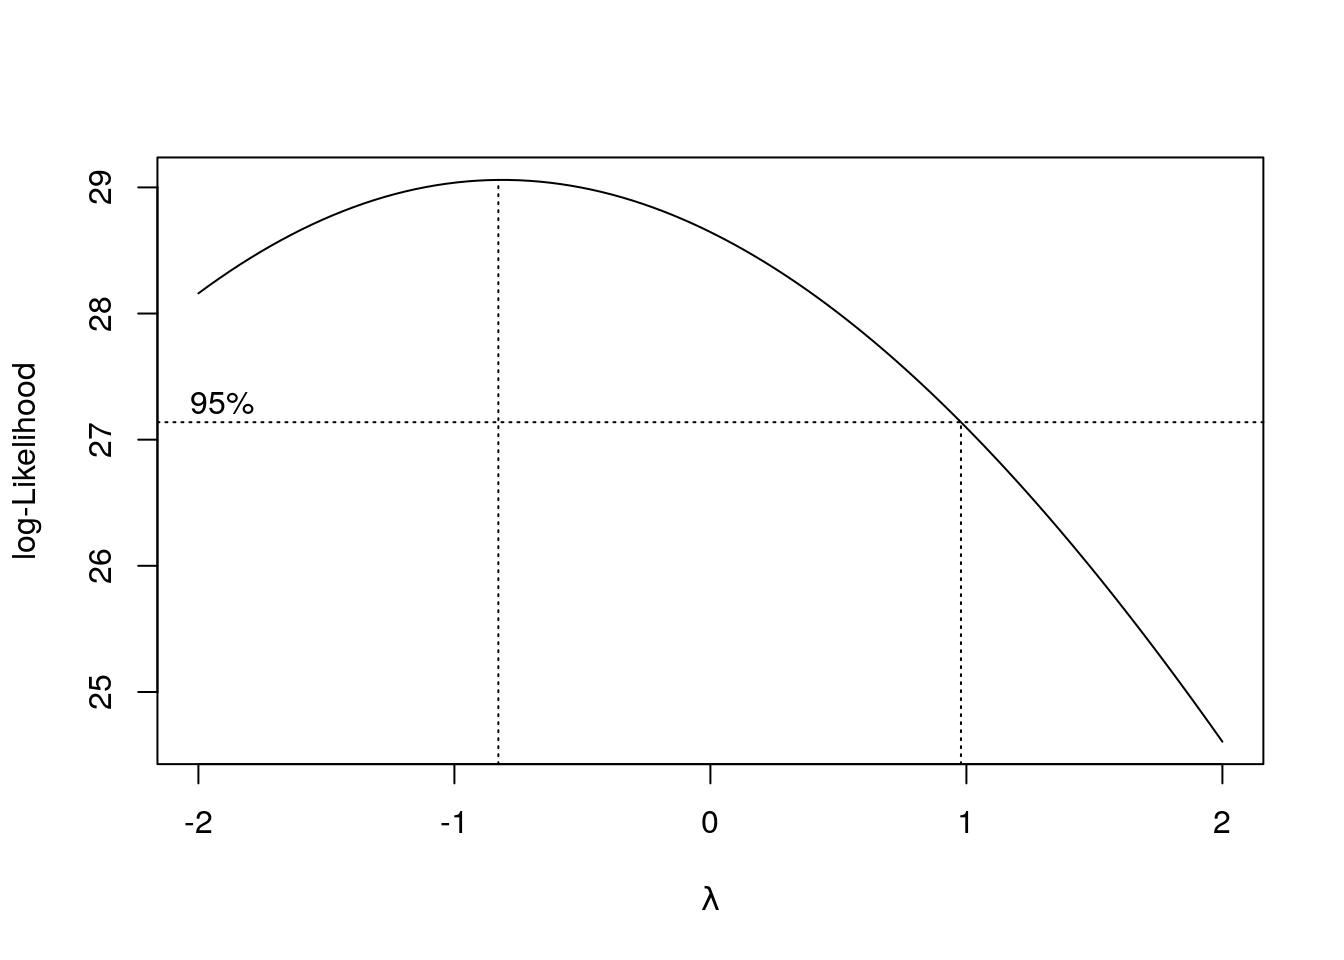
\includegraphics[width=0.3\linewidth]{hw_stat565_files/figure-latex/unnamed-chunk-41-1}
\includegraphics[width=0.3\linewidth]{hw_stat565_files/figure-latex/unnamed-chunk-41-2}
\includegraphics[width=0.3\linewidth]{hw_stat565_files/figure-latex/unnamed-chunk-41-3}
\includegraphics[width=0.3\linewidth]{hw_stat565_files/figure-latex/unnamed-chunk-41-4}
\includegraphics[width=0.3\linewidth]{hw_stat565_files/figure-latex/unnamed-chunk-41-5}
\includegraphics[width=0.3\linewidth]{hw_stat565_files/figure-latex/unnamed-chunk-41-6}

\begin{enumerate}
\def\labelenumi{(\alph{enumi})}
\setcounter{enumi}{5}
\tightlist
\item
  Report the complete code along with output here.
\end{enumerate}

\begin{Shaded}
\begin{Highlighting}[]
\CommentTok{# (a)}
\NormalTok{table_ingredients <-}\StringTok{ }\KeywordTok{read_xlsx}\NormalTok{(}\StringTok{"Exercise4_22.xlsx"}\NormalTok{);  table_ingredients}\OperatorTok{$}\NormalTok{Day <-}\StringTok{ }\KeywordTok{as.factor}\NormalTok{(table_ingredients}\OperatorTok{$}\NormalTok{Day)}
\NormalTok{table_ingredients}\OperatorTok{$}\NormalTok{Batch <-}\StringTok{ }\KeywordTok{as.factor}\NormalTok{(table_ingredients}\OperatorTok{$}\NormalTok{Batch);  table_ingredients}\OperatorTok{$}\NormalTok{Trt <-}\StringTok{ }\KeywordTok{as.factor}\NormalTok{(table_ingredients}\OperatorTok{$}\NormalTok{Trt)}
\KeywordTok{glimpse}\NormalTok{(table_ingredients)}
\CommentTok{## Observations: 25}
\CommentTok{## Variables: 4}
\CommentTok{## $ Batch <fct> 1, 1, 1, 1, 1, 2, 2, 2, 2, 2, 3, 3, 3, 3, 3, 4, 4, 4, 4,...}
\CommentTok{## $ Day   <fct> 1, 2, 3, 4, 5, 1, 2, 3, 4, 5, 1, 2, 3, 4, 5, 1, 2, 3, 4,...}
\CommentTok{## $ Trt   <fct> A, B, D, C, E, C, E, A, D, B, B, A, C, E, D, D, C, E, B,...}
\CommentTok{## $ y     <dbl> 8, 7, 1, 7, 3, 11, 2, 7, 3, 8, 4, 9, 10, 1, 5, 6, 8, 6, ...}
\NormalTok{table_ingredients}\OperatorTok\KeywordTok{ggplot}\NormalTok{(}\KeywordTok{aes}\NormalTok{(Batch,y))}\OperatorTok{+}\KeywordTok{geom_point}\NormalTok{(}\KeywordTok{aes}\NormalTok{(}\DataTypeTok{shape=}\NormalTok{Day,}\DataTypeTok{col=}\NormalTok{Trt),}\DataTypeTok{alpha=}\DecValTok{0}\NormalTok{)}\OperatorTok{+}\KeywordTok{geom_text}\NormalTok{(}\KeywordTok{aes}\NormalTok{(}\DataTypeTok{label=}\NormalTok{Day))}\OperatorTok{+}\KeywordTok{facet_grid}\NormalTok{(.}\OperatorTok{~}\NormalTok{Trt)}\OperatorTok{+}\KeywordTok{theme_light}\NormalTok{()}
\NormalTok{table_ingredients}\OperatorTok\KeywordTok{ggplot}\NormalTok{(}\KeywordTok{aes}\NormalTok{(Batch,y))}\OperatorTok{+}\KeywordTok{geom_point}\NormalTok{(}\KeywordTok{aes}\NormalTok{(}\DataTypeTok{shape=}\NormalTok{Day,}\DataTypeTok{col=}\NormalTok{Trt),}\DataTypeTok{alpha=}\DecValTok{0}\NormalTok{)}\OperatorTok{+}\KeywordTok{geom_text}\NormalTok{(}\KeywordTok{aes}\NormalTok{(}\DataTypeTok{label=}\NormalTok{Trt))}\OperatorTok{+}\KeywordTok{facet_grid}\NormalTok{(.}\OperatorTok{~}\NormalTok{Day)}\OperatorTok{+}\KeywordTok{theme_light}\NormalTok{()}
\KeywordTok{qplot}\NormalTok{(}\KeywordTok{reorder}\NormalTok{(Trt,y),y,}\DataTypeTok{data=}\NormalTok{table_ingredients)}\OperatorTok{+}\KeywordTok{geom_line}\NormalTok{(}\KeywordTok{aes}\NormalTok{(}\DataTypeTok{group=}\NormalTok{Day,}\DataTypeTok{lty=}\NormalTok{Day))}\OperatorTok{+}\KeywordTok{theme_light}\NormalTok{()}
\KeywordTok{qplot}\NormalTok{(}\KeywordTok{reorder}\NormalTok{(Trt,y),y,}\DataTypeTok{data=}\NormalTok{table_ingredients)}\OperatorTok{+}\KeywordTok{geom_line}\NormalTok{(}\KeywordTok{aes}\NormalTok{(}\DataTypeTok{group=}\NormalTok{Batch,}\DataTypeTok{lty=}\NormalTok{Batch))}\OperatorTok{+}\KeywordTok{theme_light}\NormalTok{()}
\KeywordTok{qplot}\NormalTok{(}\KeywordTok{reorder}\NormalTok{(Day,y),y,}\DataTypeTok{data=}\NormalTok{table_ingredients)}\OperatorTok{+}\KeywordTok{geom_line}\NormalTok{(}\KeywordTok{aes}\NormalTok{(}\DataTypeTok{group=}\NormalTok{Trt,}\DataTypeTok{lty=}\NormalTok{Trt))}\OperatorTok{+}\KeywordTok{theme_light}\NormalTok{()}
\KeywordTok{qplot}\NormalTok{(}\KeywordTok{reorder}\NormalTok{(Batch,y),y,}\DataTypeTok{data=}\NormalTok{table_ingredients)}\OperatorTok{+}\KeywordTok{geom_line}\NormalTok{(}\KeywordTok{aes}\NormalTok{(}\DataTypeTok{group=}\NormalTok{Trt,}\DataTypeTok{lty=}\NormalTok{Trt))}\OperatorTok{+}\KeywordTok{theme_light}\NormalTok{()}
\KeywordTok{qplot}\NormalTok{(}\KeywordTok{reorder}\NormalTok{(Day,y),y,}\DataTypeTok{data=}\NormalTok{table_ingredients)}\OperatorTok{+}\KeywordTok{geom_line}\NormalTok{(}\KeywordTok{aes}\NormalTok{(}\DataTypeTok{group=}\NormalTok{Batch,}\DataTypeTok{lty=}\NormalTok{Batch))}\OperatorTok{+}\KeywordTok{theme_light}\NormalTok{()}
\KeywordTok{qplot}\NormalTok{(}\KeywordTok{reorder}\NormalTok{(Batch,y),y,}\DataTypeTok{data=}\NormalTok{table_ingredients)}\OperatorTok{+}\KeywordTok{geom_line}\NormalTok{(}\KeywordTok{aes}\NormalTok{(}\DataTypeTok{group=}\NormalTok{Day,}\DataTypeTok{lty=}\NormalTok{Day))}\OperatorTok{+}\KeywordTok{theme_light}\NormalTok{()}
\end{Highlighting}
\end{Shaded}

\includegraphics[width=0.25\linewidth]{hw_stat565_files/figure-latex/unnamed-chunk-42-1}
\includegraphics[width=0.25\linewidth]{hw_stat565_files/figure-latex/unnamed-chunk-42-2}
\includegraphics[width=0.25\linewidth]{hw_stat565_files/figure-latex/unnamed-chunk-42-3}
\includegraphics[width=0.25\linewidth]{hw_stat565_files/figure-latex/unnamed-chunk-42-4}
\includegraphics[width=0.25\linewidth]{hw_stat565_files/figure-latex/unnamed-chunk-42-5}
\includegraphics[width=0.25\linewidth]{hw_stat565_files/figure-latex/unnamed-chunk-42-6}
\includegraphics[width=0.25\linewidth]{hw_stat565_files/figure-latex/unnamed-chunk-42-7}
\includegraphics[width=0.25\linewidth]{hw_stat565_files/figure-latex/unnamed-chunk-42-8}

\begin{Shaded}
\begin{Highlighting}[]
\CommentTok{# (b)}
\NormalTok{model_ingredients <-}\StringTok{ }\KeywordTok{aov}\NormalTok{(y}\OperatorTok{~}\NormalTok{Trt}\OperatorTok{+}\NormalTok{Day}\OperatorTok{+}\NormalTok{Batch,}\DataTypeTok{data =}\NormalTok{table_ingredients)}
\KeywordTok{summary}\NormalTok{(model_ingredients)}
\CommentTok{##             Df Sum Sq Mean Sq F value   Pr(>F)    }
\CommentTok{## Trt          4 141.44   35.36  11.309 0.000488 ***}
\CommentTok{## Day          4  12.24    3.06   0.979 0.455014    }
\CommentTok{## Batch        4  15.44    3.86   1.235 0.347618    }
\CommentTok{## Residuals   12  37.52    3.13                     }
\CommentTok{## ---}
\CommentTok{## Signif. codes:  0 '***' 0.001 '**' 0.01 '*' 0.05 '.' 0.1 ' ' 1}
\end{Highlighting}
\end{Shaded}

\begin{Shaded}
\begin{Highlighting}[]
\CommentTok{# (d)}
\KeywordTok{TukeyHSD}\NormalTok{(model_ingredients,}\DataTypeTok{conf.level =} \FloatTok{0.95}\NormalTok{)}
\CommentTok{##   Tukey multiple comparisons of means}
\CommentTok{##     95% family-wise confidence level}
\CommentTok{## }
\CommentTok{## Fit: aov(formula = y ~ Trt + Day + Batch, data = table_ingredients)}
\CommentTok{## }
\CommentTok{## $Trt}
\CommentTok{##     diff        lwr        upr     p adj}
\CommentTok{## B-A -2.8 -6.3646078  0.7646078 0.1539433}
\CommentTok{## C-A  0.4 -3.1646078  3.9646078 0.9960012}
\CommentTok{## D-A -5.0 -8.5646078 -1.4353922 0.0055862}
\CommentTok{## E-A -5.2 -8.7646078 -1.6353922 0.0041431}
\CommentTok{## C-B  3.2 -0.3646078  6.7646078 0.0864353}
\CommentTok{## D-B -2.2 -5.7646078  1.3646078 0.3365811}
\CommentTok{## E-B -2.4 -5.9646078  1.1646078 0.2631551}
\CommentTok{## D-C -5.4 -8.9646078 -1.8353922 0.0030822}
\CommentTok{## E-C -5.6 -9.1646078 -2.0353922 0.0023007}
\CommentTok{## E-D -0.2 -3.7646078  3.3646078 0.9997349}
\CommentTok{## }
\CommentTok{## $Day}
\CommentTok{##     diff       lwr      upr     p adj}
\CommentTok{## 2-1 -1.0 -4.564608 2.564608 0.8936609}
\CommentTok{## 3-1 -1.2 -4.764608 2.364608 0.8166339}
\CommentTok{## 4-1 -1.6 -5.164608 1.964608 0.6212723}
\CommentTok{## 5-1  0.2 -3.364608 3.764608 0.9997349}
\CommentTok{## 3-2 -0.2 -3.764608 3.364608 0.9997349}
\CommentTok{## 4-2 -0.6 -4.164608 2.964608 0.9816047}
\CommentTok{## 5-2  1.2 -2.364608 4.764608 0.8166339}
\CommentTok{## 4-3 -0.4 -3.964608 3.164608 0.9960012}
\CommentTok{## 5-3  1.4 -2.164608 4.964608 0.7232162}
\CommentTok{## 5-4  1.8 -1.764608 5.364608 0.5188508}
\CommentTok{## }
\CommentTok{## $Batch}
\CommentTok{##     diff       lwr      upr     p adj}
\CommentTok{## 2-1  1.0 -2.564608 4.564608 0.8936609}
\CommentTok{## 3-1  0.6 -2.964608 4.164608 0.9816047}
\CommentTok{## 4-1  2.0 -1.564608 5.564608 0.4225127}
\CommentTok{## 5-1 -0.2 -3.764608 3.364608 0.9997349}
\CommentTok{## 3-2 -0.4 -3.964608 3.164608 0.9960012}
\CommentTok{## 4-2  1.0 -2.564608 4.564608 0.8936609}
\CommentTok{## 5-2 -1.2 -4.764608 2.364608 0.8166339}
\CommentTok{## 4-3  1.4 -2.164608 4.964608 0.7232162}
\CommentTok{## 5-3 -0.8 -4.364608 2.764608 0.9489243}
\CommentTok{## 5-4 -2.2 -5.764608 1.364608 0.3365811}
\end{Highlighting}
\end{Shaded}

\begin{Shaded}
\begin{Highlighting}[]
\CommentTok{# (e)}
\NormalTok{table_ingredients}\OperatorTok{$}\NormalTok{student_resid <-}\StringTok{ }\KeywordTok{rstudent}\NormalTok{(model_ingredients)}
\KeywordTok{ols_plot_resid_hist}\NormalTok{(}\KeywordTok{lm}\NormalTok{(y}\OperatorTok{~}\NormalTok{Trt}\OperatorTok{+}\NormalTok{Day}\OperatorTok{+}\NormalTok{Batch,}\DataTypeTok{data =}\NormalTok{table_ingredients))}
\KeywordTok{ols_plot_resid_stud_fit}\NormalTok{(}\KeywordTok{lm}\NormalTok{(y}\OperatorTok{~}\NormalTok{Trt}\OperatorTok{+}\NormalTok{Day}\OperatorTok{+}\NormalTok{Batch,}\DataTypeTok{data =}\NormalTok{table_ingredients))}
\KeywordTok{ols_plot_resid_qq}\NormalTok{(}\KeywordTok{lm}\NormalTok{(y}\OperatorTok{~}\NormalTok{Trt}\OperatorTok{+}\NormalTok{Day}\OperatorTok{+}\NormalTok{Batch,}\DataTypeTok{data =}\NormalTok{table_ingredients))}
\KeywordTok{ggplot}\NormalTok{(table_ingredients,}\KeywordTok{aes}\NormalTok{(Trt,student_resid))}\OperatorTok{+}\KeywordTok{geom_dotplot}\NormalTok{(}\DataTypeTok{binaxis =} \StringTok{"y"}\NormalTok{, }\DataTypeTok{stackdir =} \StringTok{"center"}\NormalTok{,}\DataTypeTok{binwidth=}\FloatTok{0.1}\NormalTok{,}\DataTypeTok{alpha=}\FloatTok{0.6}\NormalTok{)}\OperatorTok{+}\KeywordTok{theme_light}\NormalTok{()}
\KeywordTok{ggplot}\NormalTok{(table_ingredients,}\KeywordTok{aes}\NormalTok{(Day,student_resid))}\OperatorTok{+}\KeywordTok{geom_dotplot}\NormalTok{(}\DataTypeTok{binaxis =} \StringTok{"y"}\NormalTok{, }\DataTypeTok{stackdir =} \StringTok{"center"}\NormalTok{,}\DataTypeTok{binwidth=}\FloatTok{0.1}\NormalTok{,}\DataTypeTok{alpha=}\FloatTok{0.6}\NormalTok{)}\OperatorTok{+}\KeywordTok{theme_light}\NormalTok{()}
\KeywordTok{ggplot}\NormalTok{(table_ingredients,}\KeywordTok{aes}\NormalTok{(Batch,student_resid))}\OperatorTok{+}\KeywordTok{geom_dotplot}\NormalTok{(}\DataTypeTok{binaxis =} \StringTok{"y"}\NormalTok{, }\DataTypeTok{stackdir =} \StringTok{"center"}\NormalTok{,}\DataTypeTok{binwidth=}\FloatTok{0.1}\NormalTok{,}\DataTypeTok{alpha=}\FloatTok{0.6}\NormalTok{)}\OperatorTok{+}\KeywordTok{theme_light}\NormalTok{()}
\end{Highlighting}
\end{Shaded}

\includegraphics[width=0.3\linewidth]{hw_stat565_files/figure-latex/unnamed-chunk-45-1}
\includegraphics[width=0.3\linewidth]{hw_stat565_files/figure-latex/unnamed-chunk-45-2}
\includegraphics[width=0.3\linewidth]{hw_stat565_files/figure-latex/unnamed-chunk-45-3}
\includegraphics[width=0.3\linewidth]{hw_stat565_files/figure-latex/unnamed-chunk-45-4}
\includegraphics[width=0.3\linewidth]{hw_stat565_files/figure-latex/unnamed-chunk-45-5}
\includegraphics[width=0.3\linewidth]{hw_stat565_files/figure-latex/unnamed-chunk-45-6}

\hypertarget{problem-3-3}{%
\subsubsection{Problem 3:}\label{problem-3-3}}

The data below are from a replicated Latin Square with 4 treatments: row
blocks were reused, but column blocks were not.

\begin{verbatim}
## Observations: 32
## Variables: 5
## $ Replicate <fct> 1, 1, 1, 1, 1, 1, 1, 1, 1, 1, 1, 1, 1, 1, 1, 1, 2, 2...
## $ Row       <fct> 1, 1, 1, 1, 2, 2, 2, 2, 3, 3, 3, 3, 4, 4, 4, 4, 1, 1...
## $ Col       <fct> 1, 2, 3, 4, 1, 2, 3, 4, 1, 2, 3, 4, 1, 2, 3, 4, 5, 6...
## $ Trt       <fct> D, C, B, A, B, A, D, C, C, D, A, B, A, B, C, D, B, C...
## $ y         <dbl> 44, 39, 52, 73, 26, 45, 49, 58, 67, 71, 81, 76, 77, ...
\end{verbatim}

\includegraphics[width=0.5\linewidth]{hw_stat565_files/figure-latex/unnamed-chunk-46-1}

\begin{enumerate}
\def\labelenumi{(\alph{enumi})}
\tightlist
\item
  Obtain the ANOVA table for this study and report it here.
\end{enumerate}

\begin{verbatim}
##               Df Sum Sq Mean Sq F value Pr(>F)
## Trt            3    635   211.8   0.951  0.437
## Row            3   1044   347.9   1.562  0.233
## Replicate      1     36    36.1   0.162  0.692
## Replicate:Col  6   1986   331.0   1.486  0.239
## Residuals     18   4010   222.8
\end{verbatim}

\begin{enumerate}
\def\labelenumi{(\alph{enumi})}
\setcounter{enumi}{1}
\tightlist
\item
  Test whether treatments are statistically significant at α=0.01.
  Report your conclusion and p value here.
\end{enumerate}

Set the overall hypotheses are \(H_0: \mu_1=\mu_2=\mu_3=\mu_4\) or
\(\tau_1=\tau_2=\tau_3=\tau_4\) versus \(H_1\): At least two of
\(\mu_i\)'s are different or At least one \(\tau_i\neq0\).

The ANOVA for replicated Latin-square shows that the P-value of 0.437
for treatment is larger than 0.01. We cannot reject \(H_0\). The
treatments have not significant effects on the average values of
resopnse variable at 0.01 significant level.

\hypertarget{problem-4}{%
\subsubsection{Problem 4:}\label{problem-4}}

The BIBD model with fixed effect is:\(y_{ij}=μ+τ_i+β_j+ε_{ij}\),for
i=1,2,\ldots{},a\(;\)j=1,2,\ldots{},b; \(N=kb=ra≠ab\).
\(ε_{ij} ~ iidN(0,σ^2)\);\(\sum_{i=1}^aτ_i=0\) and
\(\sum_{j=1}^bβ_j =0\);
\(y_{i.}=\sum_jy_{ij}\),\(\bar y_{.j}=\frac1k\sum_iy_{ij}=\frac{y_{.j}}k\).
Let \(Q_i=(y_{i.}-\sum_{j=1}^bn_{ij}\bar y_{.j})\) where
\(n_{ij}=\begin{cases}1& \text{if } i^{th} \text{ treatment appears in } j^{th}\text{ block}\\0&\text{Otherwise}\end{cases}\)
Prove that \(\sum_{i=1}^aQ_i=0\)

\[\sum_{i=1}^aQ_i=\sum_{i=1}^a[y_{i.}-\sum_{j=1}^bn_{ij}\bar y_{.j}]=\sum_{i=1}^a\sum_{j=1}^b y_{ij}-\sum_{j=1}^b(\bar y_{.j}\sum_{i=1}^an_{ij})=y_{..}-\sum_{j=1}^b(\frac{y_{.j}}kk)=y_{..}-y_{..}=0\]

\hypertarget{problem-5}{%
\subsubsection{Problem 5:}\label{problem-5}}

Consider the two-factor factorial model with fixed effects:
\(y_{ijk}=μ+τ_i+β_j+(τβ)_{ij}+ε_{ijk}\), for \(i=1,2,…,a\);
\(j=1,2,…,b\); \(k=1,2,…,n\)
\(ε_{ijk}\sim iid N(0,σ^2)\);\(\sum_{i=1}^aτ_i=0\) and
\(\sum_{j=1}^bβ_j=0\); \(\sum_{i=1}^a(τβ)_{ij}=0\) and
\(\sum_{j=1}^b(τβ)_{ij}=0\)
\(\bar y_{i..}=\frac1{bn}\sum_{j=1}^b\sum_{k=1}^ny_{ijk}\);
\(y_{...}=\sum_{i=1}^a\sum_{j=1}^b\sum_{k=1}^ny_{ijk}\);
\(\bar y_{...}=\frac{y_{...}}N\). Compute the \(E(SS_A)\) where
\(SS_A=bn\sum_{i=1}^a(\bar y_{i..}-\bar y_{...})^2\)

\begin{itemize}
\tightlist
\item
  For \(i=1,2,…,a\); \(j=1,2,…,b\); \(k=1,2,…,n\), for
  \(\sum_{i=1}^aτ_i=0\), \(\sum_{j=1}^bβ_j=0\);
  \(\sum_{i=1}^a(τβ)_{ij}=0\), and \(\sum_{j=1}^b(τβ)_{ij}=0\),
\end{itemize}

\(\bar y_{i..}-\bar y_{...}=\frac1{bn}\sum\limits_{j=1}^b\sum\limits_{k=1}^n(μ+τ_i+β_j+(τβ)_{ij}+ε_{ijk})-\frac1{abn}\sum\limits_{i=1}^a\sum\limits_{j=1}^b\sum\limits_{k=1}^n(μ+τ_i+β_j+(τβ)_{ij}+ε_{ijk})\)

\(=μ+τ_i+\frac1{b}\sum\limits_{j=1}^bβ_j+\frac1{b}\sum\limits_{j=1}^b(τβ)_{ij}+\frac1{bn}\sum\limits_{j=1}^b\sum\limits_{k=1}^nε_{ijk}-μ-\frac1{a}\sum\limits_{i=1}^aτ_i-\frac1{b}\sum\limits_{j=1}^bβ_j-\frac1{ab}\sum\limits_{i=1}^a\sum\limits_{j=1}^b(τβ)_{ij}-\frac1{abn}\sum\limits_{i=1}^a\sum\limits_{j=1}^b\sum\limits_{k=1}^nε_{ijk}\)

\(=τ_i+\frac1{bn}\sum_{j=1}^b\sum_{k=1}^nε_{ijk}-\frac1{abn}\sum_{i=1}^a\sum_{j=1}^b\sum_{k=1}^nε_{ijk}=τ_i+\bar ε_{i..}-\bar ε_{ijk}\)

\begin{itemize}
\tightlist
\item
  For \(τ_i\) is a constant of the \(i^th\) treatment,
  \(E{τ_i}=τ_i,V{τ_i}=0\), for \(ε_{ijk}\sim iidN(0,σ^2)\),
  \(E[ε_{ijk}]=0\)
\end{itemize}

\(E[\bar y_{i..}-\bar y_{...}]=E[τ_i+\bar ε_{i..}-\bar ε_{ijk}]=τ_i+\frac1{bn}\sum_{j=1}^b\sum_{k=1}^nE[ε_{ijk}]-\frac1{abn}\sum_{i=1}^a\sum_{j=1}^b\sum_{k=1}^nE[ε_{ijk}]=\tau_i\)

\begin{itemize}
\tightlist
\item
  For \(τ_i\) and \(ε_{ijk}\) are independent.
  \(Cov\left[τ_i,\bar ε_{i..}\right]=Cov[τ_i,\bar ε_{...}]=0\), for
  \(ε_{ijk}\sim iidN(0,σ^2)\),
  \(Cov\left[ε_{ijk},\sum_{i=1}^aε_{ijk}\right]=\sigma^2\)
\end{itemize}

\(V[\bar y_{i..}-\bar y_{...}]=\)

\[V[τ_i+\bar ε_{i..}-\bar ε_{ijk}]=V[\tau_i]+V[\frac1{bn}{\sum\limits_{j=1}^b\sum\limits_{k=1}^nε_{ijk}}]+V[\frac1{abn}{\sum\limits_{i=1}^a\sum\limits_{j=1}^b\sum\limits_{k=1}^nε_{ijk}}]+2Cov[τ_i,\bar ε_{i..}]-2Cov[τ_i,\bar ε_{...}]-2Cov[\bar ε_{i..},\bar ε_{...}]\]

\(=0+\frac{σ^2}{bn}+\frac{σ^2}{abn}+0-0-2Cov\left[\frac1{bn}{\sum\limits_{j=1}^b\sum\limits_{k=1}^nε_{ijk}},\frac1{abn}{\sum\limits_{i=1}^a\sum\limits_{j=1}^b\sum\limits_{k=1}^nε_{ijk}}\right]=\frac{σ^2}{bn}+\frac{σ^2}{abn}-\frac{2}{ab^2n^2}\sum\limits_{j=1}^b\sum\limits_{k=1}^nCov[ε_{ijk},\sum\limits_{i=1}^aε_{ijk}]\)

\(=\frac{σ^2}{bn}+\frac{σ^2}{abn}-\frac{2}{ab^2n^2}\sum\limits_{j=1}^b\sum\limits_{k=1}^nσ^2=\frac{a-1}{abn}σ^2\)

\begin{itemize}
\tightlist
\item
  For \(E[X^2]=E[X]^2+V[X]\), therefore,
\end{itemize}

\[E[SS_A]=bn\sum_{i=1}^aE[(\bar y_{i..}-\bar y_{...})^2]=bn\sum_{i=1}^a(E[\bar y_{i..}-\bar y_{...}]^2+V[\bar y_{i..}-\bar y_{...}])=bn\sum_{i=1}^a(\tau_i^2+\frac{a-1}{abn}σ^2)=bn\sum_{i=1}^aτ_i^2+(a-1)σ^2\]


\end{document}
